\documentclass[a4paper,12pt]{book}
\usepackage{graphicx}
\usepackage[export]{adjustbox}
\usepackage{subcaption}
\graphicspath{{Pics/}}
\usepackage{charter}
\usepackage{fancyhdr}
\usepackage{enumerate}
\usepackage{enumitem}
\usepackage{siunitx}
\usepackage{amssymb}
\usepackage{longtable}
\usepackage{multicol}
\usepackage{multirow}
\usepackage{hhline}
\usepackage{parskip}
\setlength{\parskip}{6pt}
\usepackage{ragged2e}
\usepackage{geometry} %margin
\geometry{left=2.1cm,right=2.1cm,top=3cm,bottom=3cm}
\usepackage{setspace}
\SetSinglespace{1.2}
\singlespacing
\renewcommand{\ttfamily}{\fontfamily{pcr}\selectfont}
%\renewcommand{\familydefault}{\rmdefault}

\usepackage[,table]{xcolor}
\definecolor{LightBlue}{cmyk}{0.16,0.03,0.04,0}
\definecolor{Title}{cmyk}{0.8,0.1,0,0.3}
\setlength{\arrayrulewidth}{0.3mm}
\setlength{\tabcolsep}{2pt}
\setlength{\headheight}{15pt}
\renewcommand{\arraystretch}{1}
\usepackage{tikz}
\usepackage{nicematrix}
\newcommand*\circled[1]{\tikz[baseline=(char.base)]{\node[shape=circle,draw,inner sep=1pt] (char) {#1};}}

\newcolumntype{s}{>{\columncolor{Title}\RaggedLeft} m{3.5em}} % columntype for chapter title
\newcolumntype{d}{>{\columncolor{LightBlue}\RaggedRight} m{\textwidth}} % columntype for code bloc
\newcolumntype{a}{>{\columncolor{LightBlue}\RaggedRight} m{0.96\textwidth}} % columntype for secondary code bloc

\usepackage{titlesec}
\usepackage[hidelinks]{hyperref}
\urlstyle{same}

\captionsetup[figure]{labelsep=period,font={bf}}
\captionsetup[table]{font={bf},labelsep=period}

\newcommand{\titlename}{}

\newcommand{\chaptertitle}[2]{ %reset chapter format
\vspace{-120pt}
\gdef\titlename{#1}
{
\SetSinglespace{1.1}
\singlespacing
\Huge\bfseries
\setlength{\tabcolsep}{8pt}
\renewcommand{\arraystretch}{1.5}
\begin{tabular}{s >{\RaggedRight}m{14.5em}}
\textcolor{white}{Chapter\newline\thechapter}&\textcolor{Title}{#2}
\end{tabular}
}
}

\newcommand{\partpic}[1]{%insert picture
    \tikz[remember picture,overlay] \node at (current page.center){\includegraphics[width=\paperwidth]{#1}};
}

\titleformat{\part} %reset part %format
{\huge\bfseries} % format
{} % label
{0em} % sep
{\Centering} % before-code

\titleformat{\chapter} %reset chapter %format
{\huge\bfseries} % format
{} % label
{0em} % sep
{\Centering} % before-code
\titlespacing{\chapter}{0pt}{0pt}{0pt}

\titleformat{\section} %reset section %format
{\Large\bfseries} % format
{\textcolor{Title}{\thesection}} % label
{0.5em} % sep
{\color{Title}} % before-code
\titlespacing{\section}{0pt}{12pt}{6pt}

\titleformat{\subsection} %reset subsection %format
{\large\bfseries} % format
{\textcolor{Title}{\thesubsection}} % label
{0.5em} % sep
{\color{Title}} % before-code
\titlespacing{\subsection}{0pt}{8pt}{6pt}

\newenvironment{term}[1]{
    \textbf{#1}

    \leftskip 1em
    \parskip 0pt
}

\newenvironment{secterm}[1]{
    \textbf{#1}

    \leftskip 2em
    \parskip 0pt
}

\newenvironment{codebloc}{ %define code bloc style
    \ttfamily\footnotesize
    \renewcommand{\arraystretch}{1}
}

\newcommand{\note}[2][NOTE]{ %Note/Tips
\vspace{6pt}
\begin{tabular}{b{\textwidth}}
\hline
\fontfamily{phv}\selectfont \textbf{#1}\\
\leftskip 1em #2\\
\hline
\end{tabular}
}

\newcommand{\secnote}[2][NOTE]{ %Note/Tips
\vspace{6pt}
\begin{tabular}{b{0.93\textwidth}}
\hline
\fontfamily{phv}\selectfont \textbf{#1}\\
\leftskip 1em #2\\
\hline
\end{tabular}
}

\title{ESP32-C3 Wireless Adventure\par \Large A comprehensive guide to IoT}
\author{Espressif Systems}
\date{\today}

\pagestyle{fancy} % reset head&foot
\fancyhead{} % clear all header fields
\renewcommand\headrulewidth{0pt}
\fancyfoot{} % clear all footer fields
\setcounter{chapter}{6}

\begin{document}

\fancyfoot[LE]{\fontfamily{cmss}\selectfont{\textbf{\thepage} \ \textit{ESP32-C3 Wireless Adventure: A comprehensive guide to IoT}}}
\fancyfoot[RO]{\fontfamily{cmss}\selectfont{\textit{Chapter \thechapter. \titlename} \ \textbf{\thepage}}}

{\makeatletter
\let\ps@plain\ps@empty
\makeatother
\part[Wireless Communication and Control]{\partpic{Starting/3c}}
}

\chapter[Wi-Fi Configuration and Connection]{\chaptertitle{Wi-Fi Configuration and Connection}{Wi-Fi Configuration and\newline Connection}}

\vspace{36pt}
In this chapter, we’ll focus on the specifications of Wi-Fi network configuration and connection, from the basics of Wi-Fi and Bluetooth to the common methods for configuring Wi-Fi network. Then, examples will be given to help you better understand its operating mechanism, and ways of smart Wi-Fi configuration. Finally, we’ll lead you to a practice of smart Wi-Fi configuration with the Smart Light project based on ESP32-C3.

Since the wireless communication technology has gone through a long history, many documents have delved deeply into this topic. Therefore, this chapter will only provide a brief introduction. For details, please see the references listed at the end of this book.

\section{Basics of Wi-Fi}
This section will walk you through the Wi-Fi technology from the following aspects:

\begin{itemize}
    \item What is Wi-Fi?
    \item How does Wi-Fi evolve?
    \item What do the Wi-Fi concepts mean? 
    \item How does Wi-Fi connection work?
\end{itemize}

\subsection{Introduction to Wi-Fi}
Wi-Fi is a trademark of wireless communication technology owned by the Wi-Fi Alliance (WFA), which supervises Wi-Fi certification. It is a family of wireless network protocols based on the IEEE 802.11 standards. Products passing rigorous testings will be given the Wi-Fi CERTIFIED™ seal to prove that they have met industry-agreed standards for interoperability, security, and a range of application specific protocols.

Compared with other wireless communication technologies, Wi-Fi boasts wider coverage, better penetrating ability through walls, and higher throughput.

\subsection{Evolution of IEEE 802.11}
As Wi-Fi users, we should have heard about IEEE 802.11 more or less. But what does it exactly mean?

\textbf{IEEE} is the abbreviation of the Institute of Electrical and Electronics Engineers. \textbf{802} is a committee in the institute for networking standards, also known as the LMSC – LAN/MAN Standards Committee. The committee covers such a big family of standards that it needs to be divided into groups devoted to specific areas. Each group has its own number (the one following “802”, separated by a dot), so \textbf{802.11} refers to the 11th group of committee 802, which develops the Medium Access Control (MAC) protocols and Physical Layer (PHY) specifications of wireless local area networks (WLANs). IEEE 802.11 has experienced several “amendments”, as shown in Table 7.1.

\begin{table}[h!]
    \renewcommand{\arraystretch}{1.5}
    \caption{Generations of IEEE 802.11}
    \begin{tabular}{|>{\Centering}m{4.5em}|>{\Centering}m{6.5em}|>{\Centering}m{10.5em}|>{\Centering}m{6em}|>{\Centering}m{6em}|>{\Centering}m{4em}|}
        \hline
        \rowcolor{LightBlue} \textbf{Version}&\textbf{Frequency Range (GHz)}&\textbf{Channel Bandwidth\newline (MHz)}&\textbf{Rate (Mbit/s)}&\textbf{Modulation Method}&\textbf{Alias}\\
        \hline
        802.11a&5&20&54&OFDM$^2$&—\\
        \hline
        802.11b&2.4&22&11&CCK$^3$/DSSS$^4$&—\\
        \hline
        802.11g&2.4&20&54&OFDM&—\\
        \hline
        802.11n&2.4, 5&20, 40&72-600 (MIMO$^1$:4×4)&OFDM&Wi-Fi 4\\
        \hline
        802.11ac&5&20, 40, 80, 80+80, 160&433-1733 (MIMO:4×4)&OFDM&Wi-Fi 5\\
        \hline
        802.11ax&2.4, 5&20, 40, 80, 80+80, 160&600-2401 (MIMO:4×4)&OFDMA$^5$&Wi-Fi 6\\
        \hline
    \end{tabular}
\end{table}

\textbf{Table notes:}

\begin{enumerate}[label=$^\arabic*$]
    \item MIMO: Multiple Input Multiple Output.
    \item OFDM: Orthogonal Frequency Division Multiplexing.
    \item CCK: Complementary Code Keying.
    \item DSSS: Direct Sequence Spread Spectrum.
    \item OFDMA: Orthogonal Frequency Division Multiple Access.
\end{enumerate}

\subsection{Wi-Fi Concepts}
In this section, we’ll introduce the network technologies related to IEEE 802.11, including the Open System Interconnection Reference Model (OSI/RM) and physical components of IEEE 802.11.

\begin{term}{Open System Interconnection Reference Model (OSI/RM)}
    In OSI/RM, the computer network system is conceived as a seven-layer framework. Their names and relationships are shown in Figure 7.1.

    \begin{figure}[!h]
        \centering
        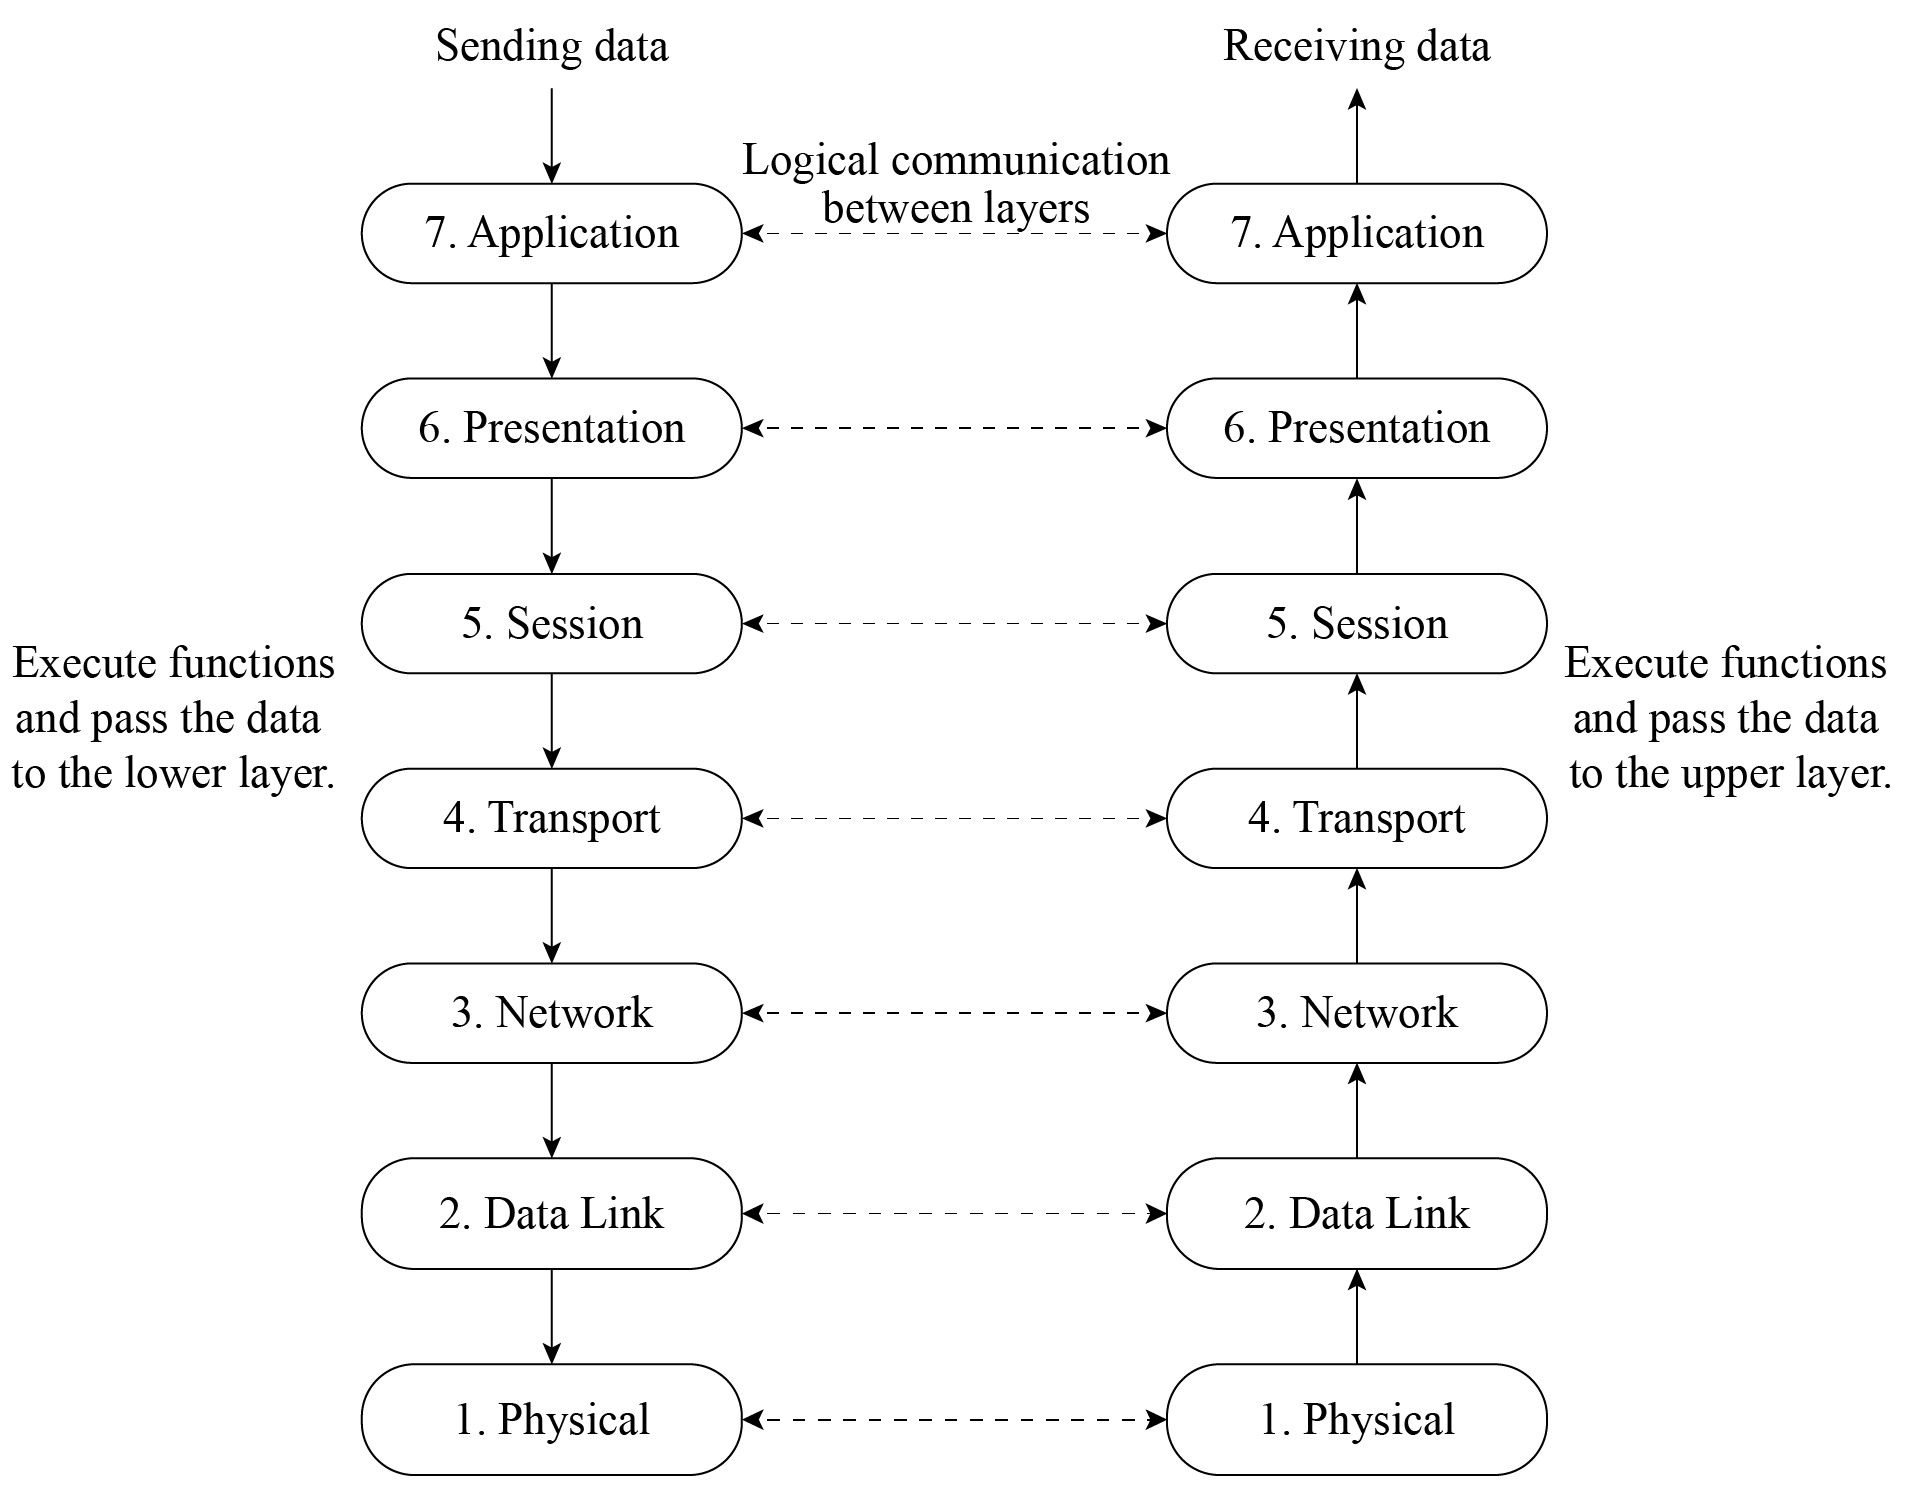
\includegraphics[width=0.8\textwidth]{D7Z/7-1}
        \caption{Architecture of OSI/RM}
    \end{figure}
\end{term}

\begin{term}{Physical components of IEEE 802.11}
    IEEE 802.11 architecture consists of four major physical components, as shown in Figure 7.2.

    \begin{figure}[!h]
        \centering
        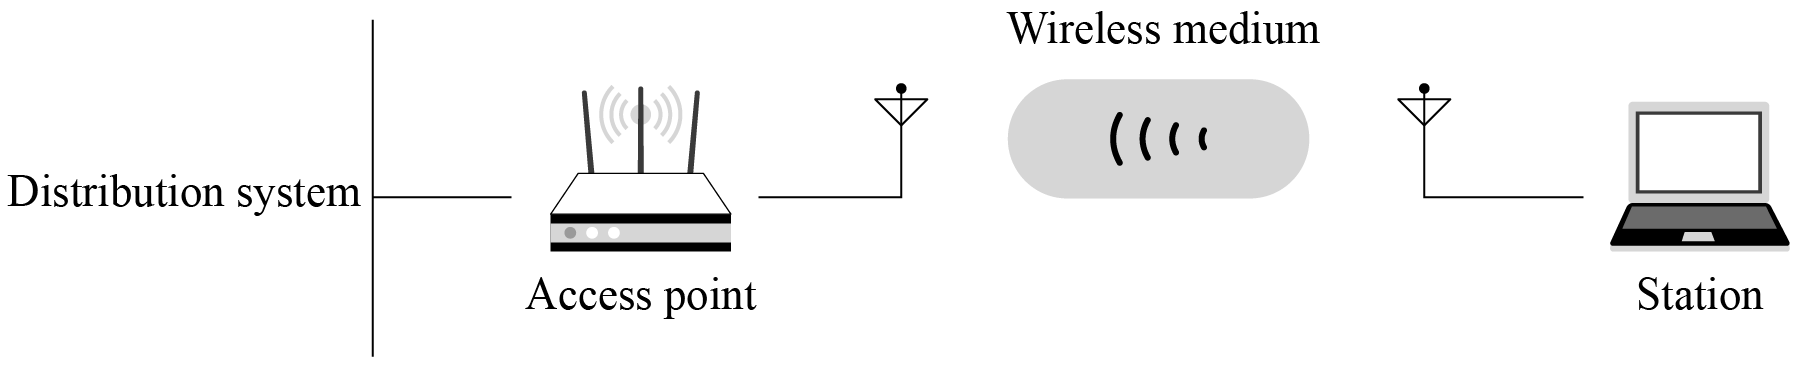
\includegraphics[width=0.8\textwidth]{D7Z/7-2}
        \caption{Physical components of IEEE 802.11}
    \end{figure}

    \parskip 6pt
    \begin{secterm}{Wireless Medium (WM)}
        WMs refer to the physical layer where wireless MAC frame data is transmitted. Initially, two radio frequency (RF) physical layers and one infrared physical layer were introduced, but the RF layers turned out to be more popular.
    \end{secterm}

    \begin{secterm}{Stations (STA)}
        Stations comprise all devices and equipments that are connected to the wireless LAN. Battery-operated laptops and handheld computers are typical STAs, but “portable” is not a must. In some cases, desktops are also connected to wireless LANs to avoid pulling new cables.
    \end{secterm}

    \begin{secterm}{Access Points (AP)}
        As a branch of STA, AP provides access to distribution services for associated STAs.
    \end{secterm}

    \begin{secterm}{Distribution System (DS)}
        When several APs are connected to cover a larger area, they have to communicate with each other to track the movements of mobile stations. This is conducted through the distribution system, an external data network. It is responsible for transmitting data frames to their destinations.
    \end{secterm}
\end{term}

\begin{term}{Building wireless networks}
    The physical components above constitute a wireless network. The basic building block of an IEEE 802.11 network is the Basic Service Set (BSS). It comes in two categories, the Independent BSS and the Infrastructure BSS, as shown in Figure 7.3.

    \begin{figure}[!h]
        \centering
        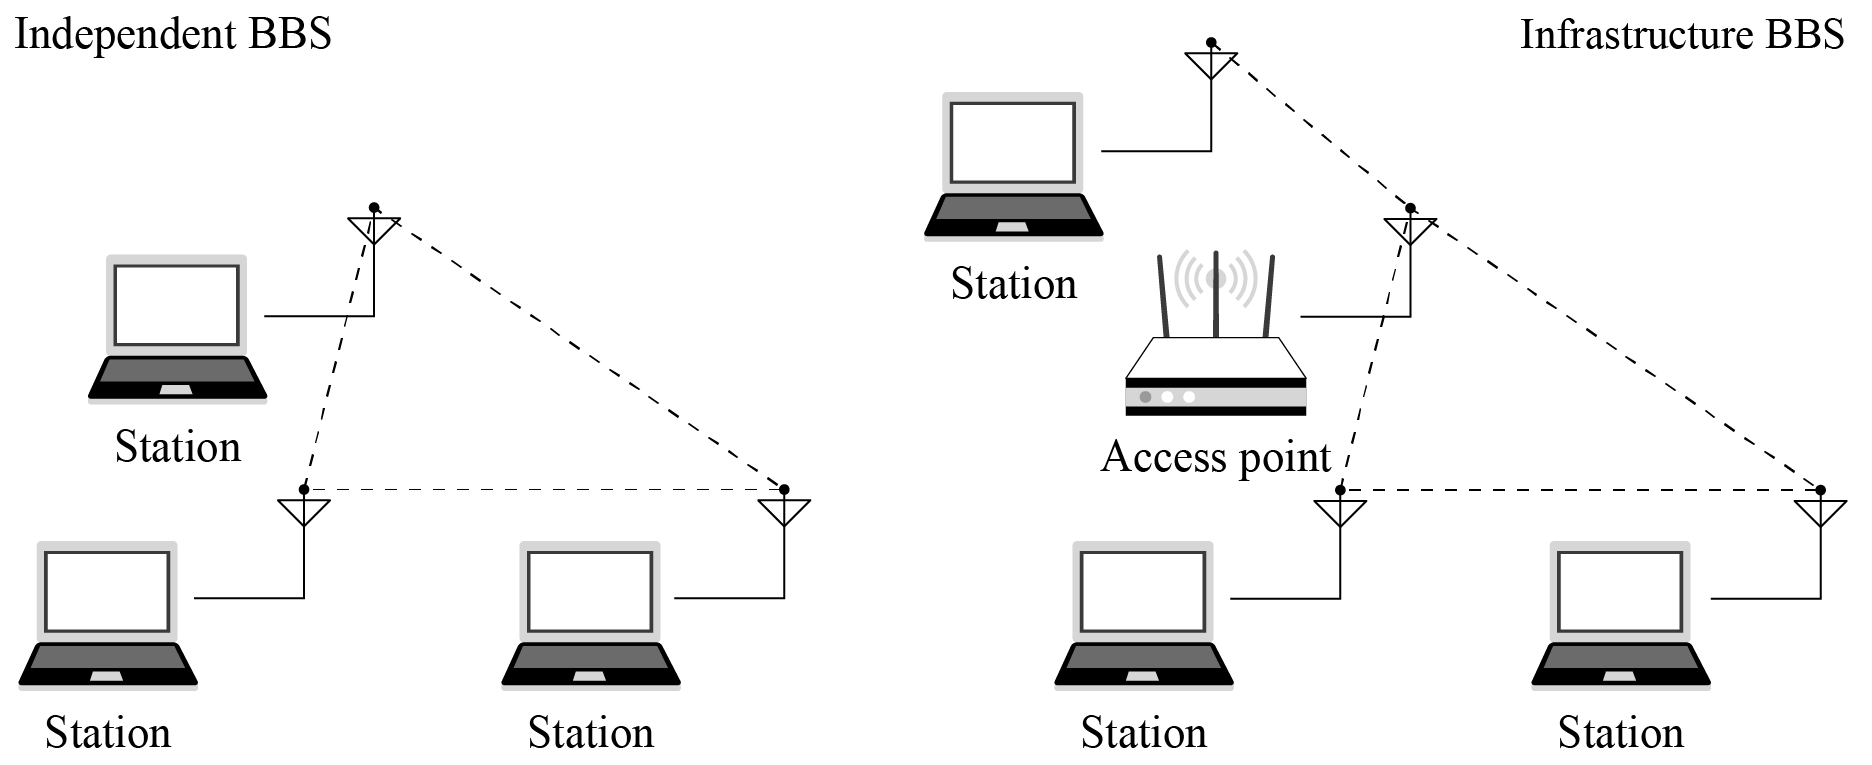
\includegraphics[width=0.8\textwidth]{D7Z/7-3}
        \caption{Independent BSS and infrastructure BSS}
    \end{figure}

    \parskip 6pt
    \begin{secterm}{Independent BSS}
        Stations in an independent BSS communicate with each other directly without AP.
    \end{secterm}

    \begin{secterm}{Infrastructure BSS}
        In an infrastructure BSS, STAs must associate with an AP to obtain network services. APs function as the control centre of the set. This is the most common network architecture. Every STA needs to go through association and authorisation before joining a certain BSS. Infrastructure BSS is the most common network architecture.
    \end{secterm}

    Network architectures are accompanied with identifications:

    \begin{secterm}{BSS Identification (BSSID)}
        Each BSS has a physical address for identification, called BSSID. For an Infrastructure BSS, the BSSID is the MAC address of the AP. It comes with a factory default value and can be changed according a fixed naming format.
    \end{secterm}

    \begin{secterm}{Service Set Identification (SSID)}
        Each AP has an identifier for user identification. In most cases, one BSSID is associated with one SSID. It is usually a readable string, which is what we call the Wi-Fi name.
    \end{secterm}
\end{term}

\subsection{Wi-Fi Connection}
An STA first searches for nearby wireless networks through active or passive scanning, then establishes a connection with an AP after authentication and association, and finally accesses the wireless LAN. Figure 7.4 shows the process of Wi-Fi connection.

\begin{figure}[!h]
    \centering
    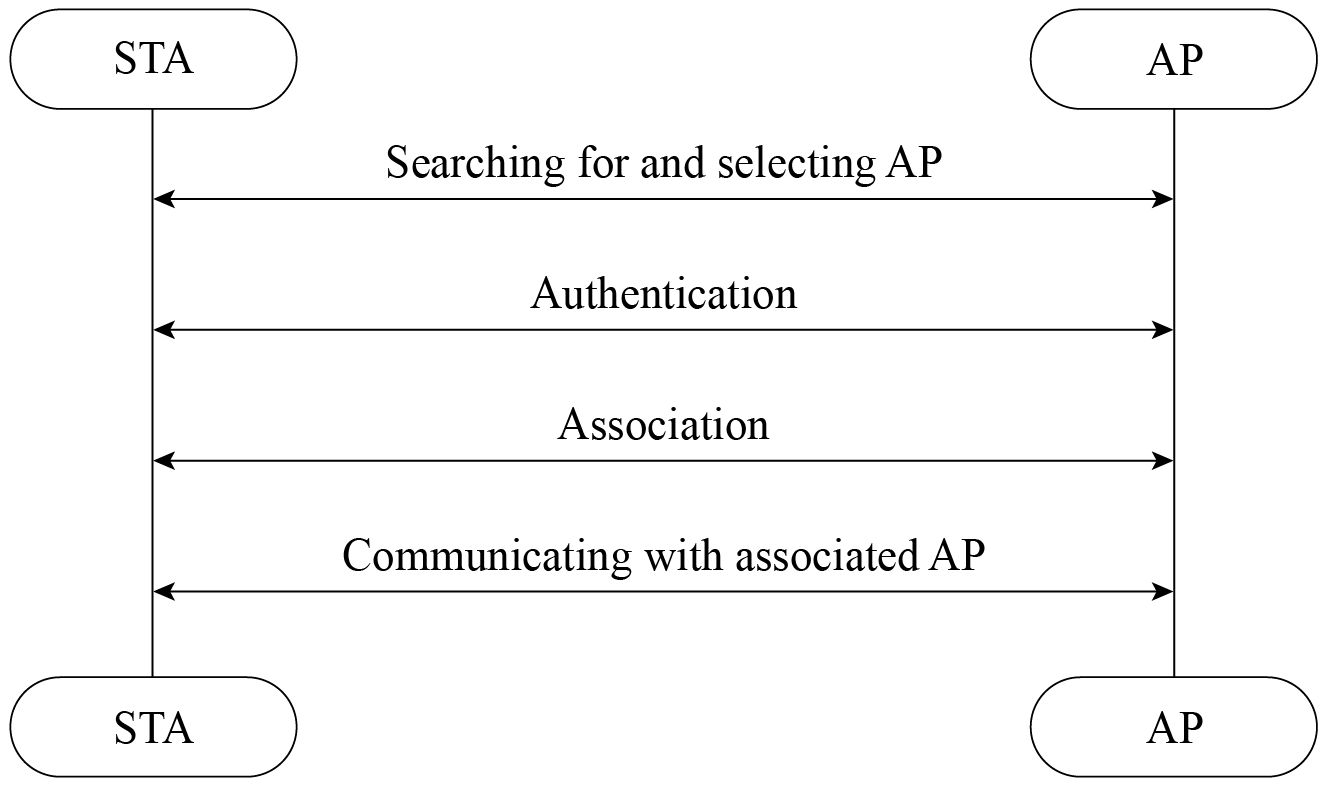
\includegraphics[width=0.6\textwidth]{D7Z/7-4}
    \caption{Process of Wi-Fi connection}
\end{figure}

\textbf{1. Scanning}

An STA can actively or passively scan wireless networks.

\begin{term}{Passive scanning}
    Passive scanning refers to discovering wireless networks nearby through monitoring the beacon frames periodically sent by an AP. It is recommended when users need to save power.
\end{term}

\begin{term}{Active scanning}
    During active scanning, the STA actively sends out probe requests and receives probe responses from the AP. It is further devided into two modes based on the involvement of SSID.

    \parskip 6pt
    \begin{secterm}{Active scanning without SSID}
        The STA periodically sends out probe requests through supported channels to search for wireless networks. APs that receive the probe request will return probe responses, which carry the information of available wireless networks. This enables an STA to obtain all the available wireless services nearby.
    \end{secterm}

    \begin{secterm}{Active scanning with specific SSIDs}
        If the STA needs to configure a wireless network to be connected or has accessed a wireless network before, it will periodically send out probe requests with configuration information or the SSID of the accessed wireless network. When an AP with specific SSID receives the request, it will return a probe response. In this way, an STA can actively access a specified wireless network.
    \end{secterm}

    For hidden APs, active scanning with specific SSID is recommended.
\end{term}

\textbf{2. Authentication}

When the STA finds an available wireless network, it will select one of the APs with matching SSID according to certain connection strategy, such as selecting the one with strongest signal or with matching MAC address. The next step is authentication. There is open authentication and non-open authentication.

\begin{term}{Open authentication}
    Essentially, open authentication requires no authentication or encryption. Any STA can access the network. The AP does not verify STA’s identity in this process, as shown in Figure 7.5.

    \begin{figure}[!h]
        \centering
        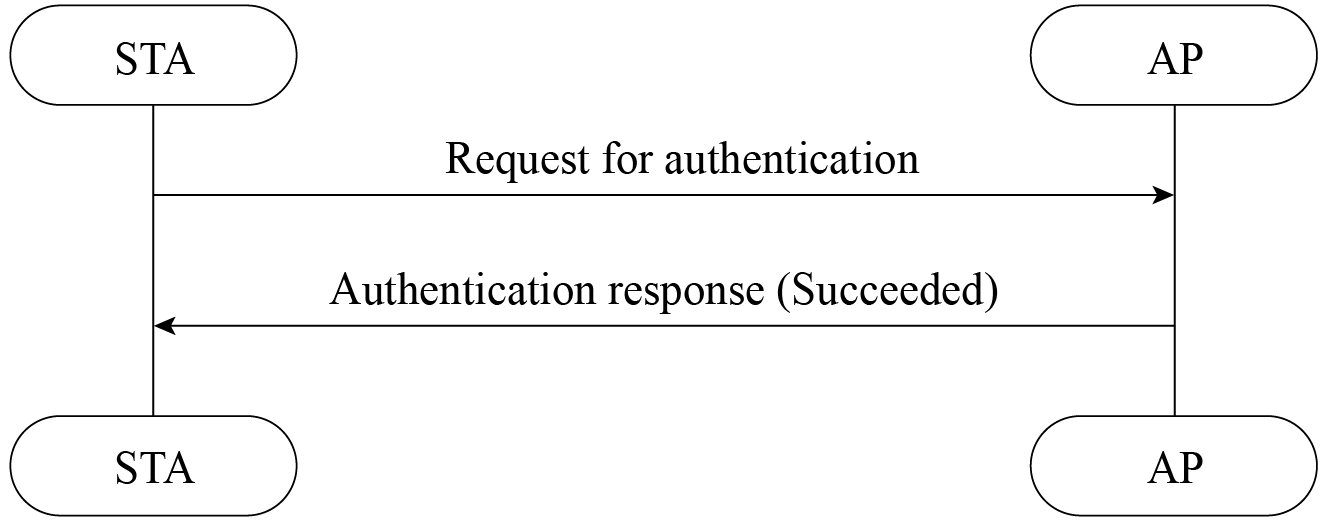
\includegraphics[width=0.6\textwidth]{D7Z/7-5}
        \caption{Process of open authentication}
    \end{figure}

    The STA sends a request for authentication, and the AP returns the result. If the result reads “Success”, then the authentication is completed.
\end{term}

\begin{term}{Non-open authentication}
    Non-open authentication includes shared key authentication, Wi-Fi Protected Access (WPA), and Robust Security Network (RSN).

    \parskip 6pt
    \begin{secterm}{Shared key}
        Shared key authentication is based on the Wired Equivalent Privacy (WEP) method. It is a basic encryption technology with security flaws.
        
        STAs and APs can only interpret the data transmitted between each other when they have the same key configured. There are 64-bit keys and 128-bit keys. Users can set up to four groups of different keys. Figure 7.6 shows the process of shared key authentication.

        \begin{figure}[!h]
            \centering
            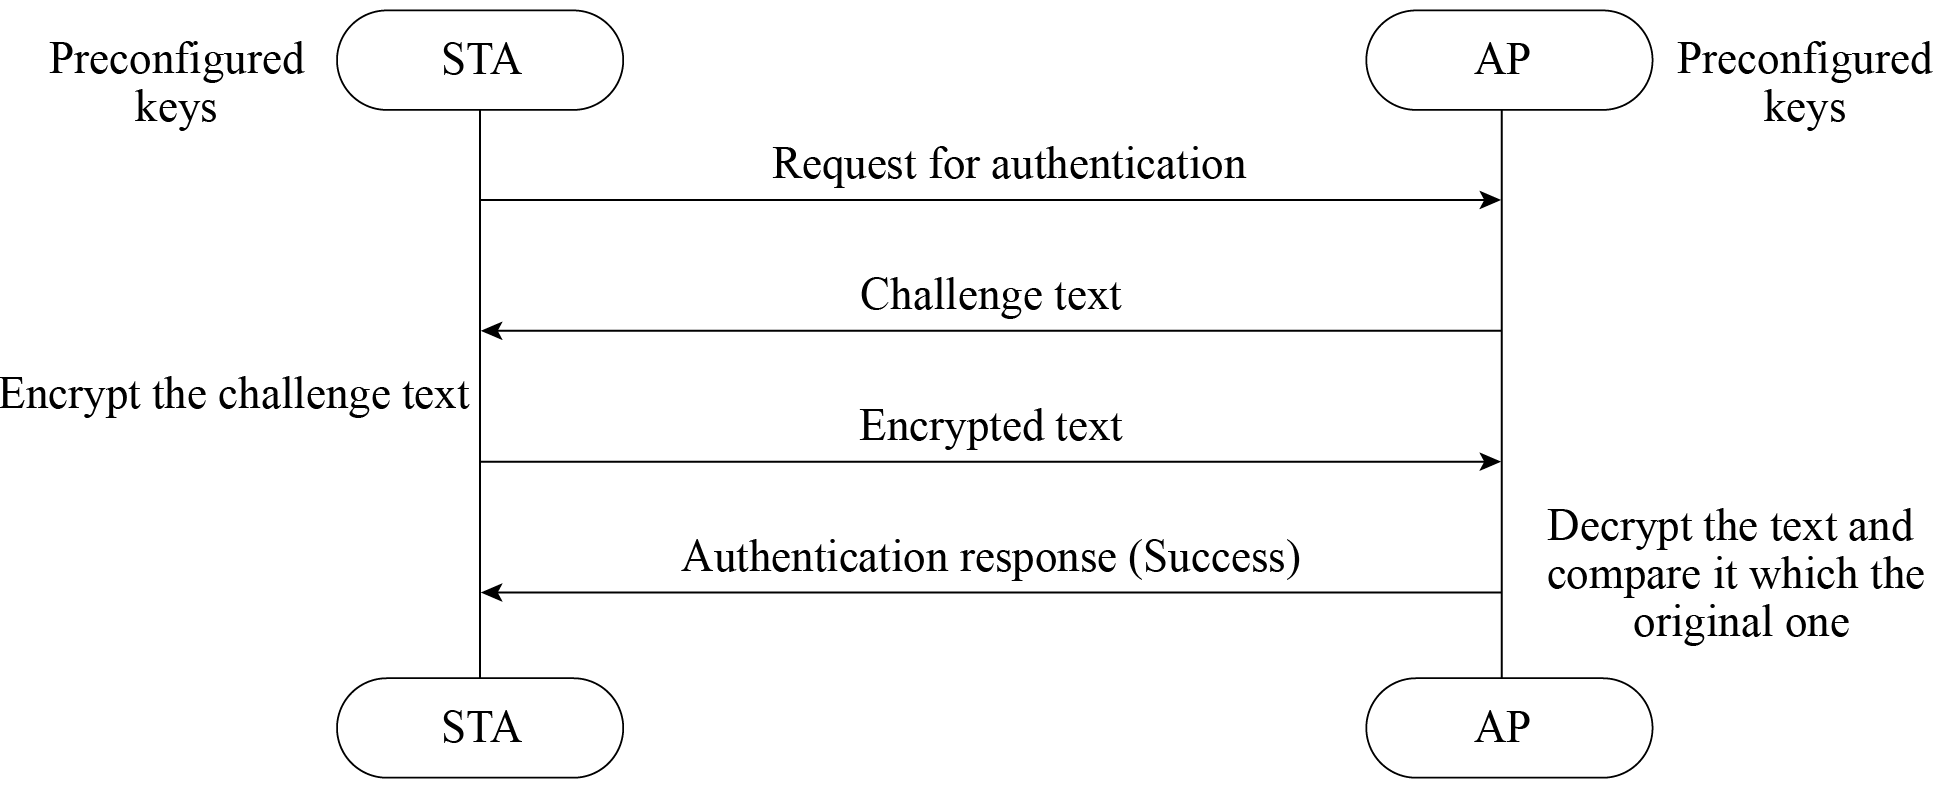
\includegraphics[width=0.85\textwidth]{D7Z/7-6}
            \caption{Process of shared key authentication}
        \end{figure}

        The STA sends an authentication request to the AP. Then the AP generates a challenge text and sends it to the STA. The STA uses its preconfigured keys to encrypt the text and sends it back. The AP uses its preconfigured keys to decrypt the text and compares it with the original text. If the two texts are identical, then the authentication is completed.
    \end{secterm}

    \begin{secterm}{Wi-Fi Protected Access (WPA)}
        WPA is an intermediate solution to replace WEP before the official release of IEEE 802.11i. It uses a new Message Integrity Check (MIC) algorithm to replace the CRC algorithm in WEP. It also adopts the Temporal Key Integrity Protocol (TKIP) to generate different keys for different MAC frames. TKIP is a transitional encryption protocol and has proved of low security.
    \end{secterm}

    \begin{secterm}{Robust Security Network (RSN)}
        The WFA calls RSN the WPA2. It adopts a new encryption method, the Counter Mode with CBC-MAC Protocol (CCMP), a block security protocol based on the Advanced Encryption Standard (AES). We will expound on this later along with authorisation.
    \end{secterm}

    \begin{secterm}{Wi-Fi Protected Access 3 (WPA3)}
        Although WPA2 consolidates Wi-Fi networks to a certain extent, new security vulnerabilities keep emerging, such as offline dictionary attacks, brute force attacks, and key reinstallation attacks (KRACK). To this end, the WFA released the WPA3 in 2018, a new generation of Wi-Fi encryption protocol that mitigates the risks in WPA2 and provides new features. Compared with WPA2, WPA3 has the following advantages:

        \parskip 6pt
        \begin{itemize}
            \item The use of AES encryption is mandatory instead of TKIP.
            \item Management frames are protected.
            \item The more secure method, Simultaneous Authentication of Equals (SAE), is used to replace the pre-shared key (PSK) authentication in WPA2.
            
            First, SAE denies services for STAs that repeatedly try to connect to the AP, preventing brute-force attacks or password cracking. Second, its forward secrecy function ensures that the key will be changed frequently and automatically, so that even if the most recent key is hacked, only a minimal amount of data will be exposed. Last, SAE considers devices as peers. Either party can initiate a handshake and send authentication information independently, cancelling the message exchange process, thus leaving no opportunity for KRACKs.
            \item 192-bit security suite is used to strengthen password protection.
            \item HMAC-SHA-384 algorithm is used to export and confirm keys in the four-way handshake phase.
            \item Galois-Counter Mode Protocol-256 (GCMP-256) is used to protect wireless traffic after STAs go online.
            \item Galois Message Authentication Code-256 (GMAC-256) of GCMP is used to protect multicast management frames.
            \item WPA3 introduces a Wi-Fi Enhanced Open authentication mode – the Opportunistic Wireless Encryption (OWE) – which allows for connection without password, retaining the facilitation for accessing open networks. It uses the Diffie-Hellman key exchange algorithm to encrypt data on the Wi-Fi network, thereby protecting data exchange between STAs and the Wi-Fi network.
        \end{itemize}
    \end{secterm}
\end{term}

\textbf{3. Association}

After the AP returns successful authentication result to the STA, the next step is association to get full network access, as shown in Figure 7.7.

\begin{figure}[!h]
    \centering
    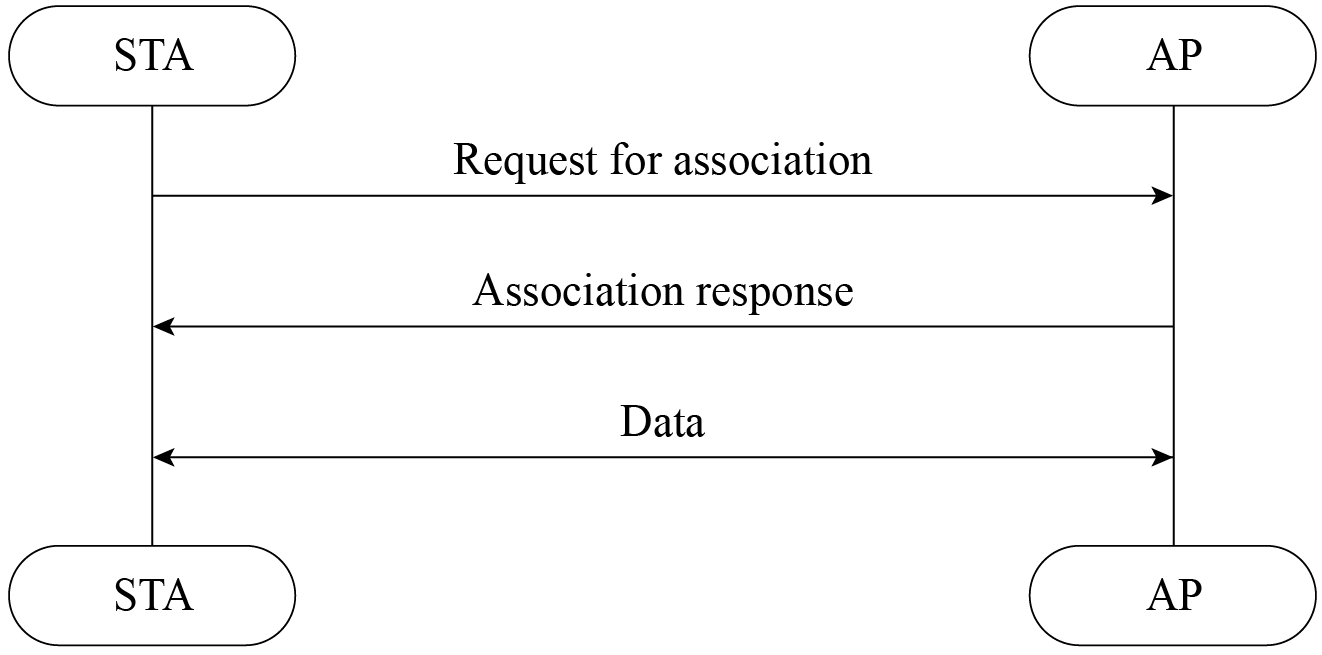
\includegraphics[width=0.6\textwidth]{D7Z/7-7}
    \caption{Process of association}
\end{figure}

\textbf{4. Authorisation}

After scanning, authentication, and association, let’s focus on the last step – authorisation. In this section, we’ll introduce the Extensible Authentication Protocol (EAP), and the key agreement, the four-way handshake protocol.

\begin{term}{Extensible Authentication Protocol (EAP)}
    EAP is the most basic security protocol for identity verification, which is not only a protocol, but also a protocol framework. Based on this protocol framework, various authentication methods are well supported. Supplicants send identity verification requests to the Authenticator through EAP over LAN (EAPOL), and get allowed to use the network once the verification succeeds. Figure 7.8 shows the architecture of EAP.
    
    \parskip 6pt
    This book only touches the basics about EAP. To learn more, please refer to RFC 3748.

    \begin{figure}[!h]
        \centering
        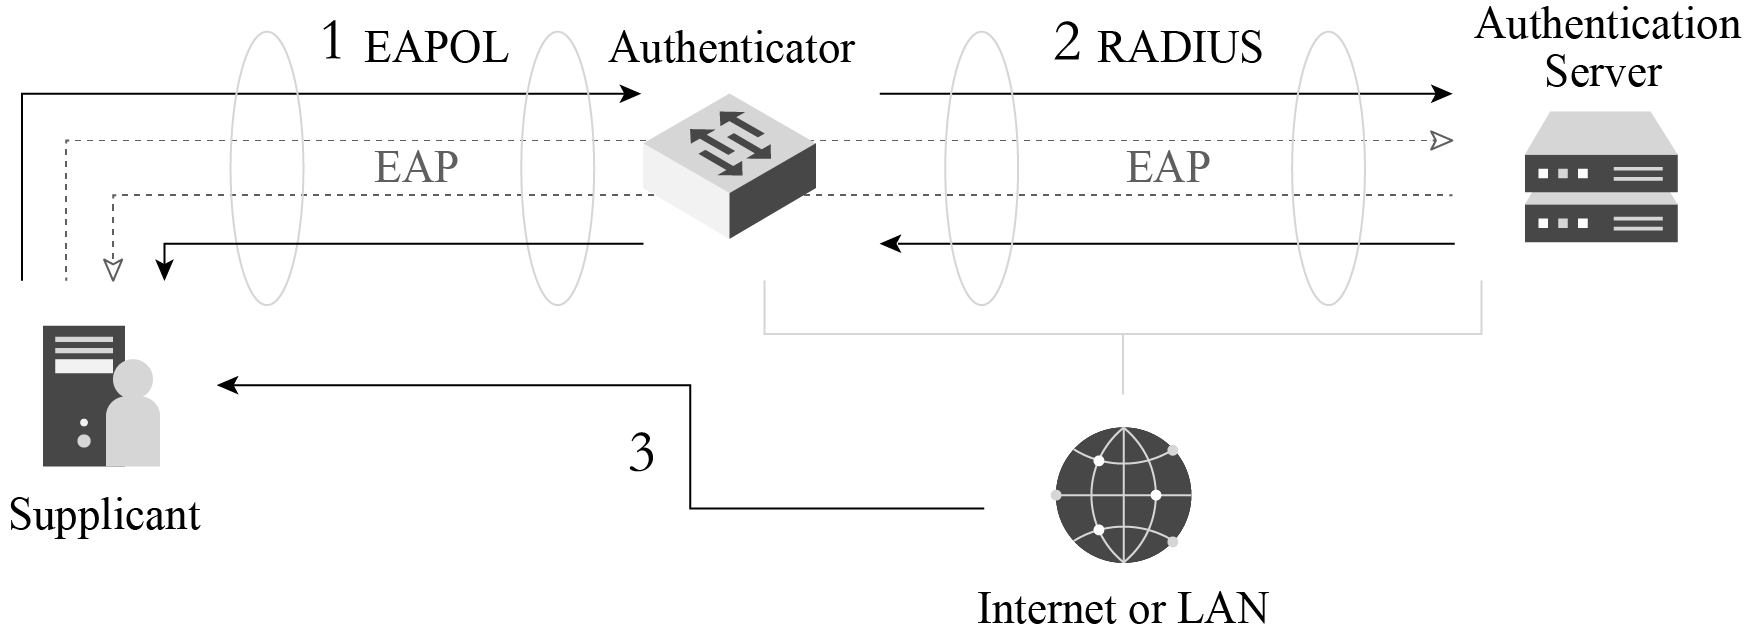
\includegraphics[width=0.75\textwidth]{D7Z/7-8}
        \caption{EAP architecture}
    \end{figure}

    \begin{itemize}
        \item \textbf{Supplicant}: the entity that initiates an authentication request. For wireless networks, an STA is a Supplicant.
        \item \textbf{Authenticator}: the entity that responds to an authentication request. For wireless networks, an AP is an Authenticator.
        \item \textbf{Backend Authentication Server (BAS)}: In some cases, such as in enterprise applications, Authenticator does not directly handle authorisation. Instead, it sends the authentication request to the BAS. This is how the EAP extends its range of application.
        \item \textbf{Authentication, Authorization, and Accounting (AAA)}: another EAP-based protocol. The entity implementing this protocol is a certain type of BAS, for example, the RADIUS server.
        \item \textbf{EAP server}: This is what actually handles authorisation. If there is no BAS, the Authenticator plays as the EAP server, otherwise the BAS will serve the purpose.
    \end{itemize}
\end{term}

\begin{term}{Key agreement}
    Robust Secure Network Association (RSNA) is a set of procedures defined in IEEE 802.11 to ensure wireless network security. It consists of \textbf{data encryption} and \textbf{integrity verification}. RSNA uses the above mentioned TKIP and CCMP. The Temporary Key (TK) used in TKIP and CCMP comes from the key derivation function defined by RSNA. Based on IEEE 802.1X, RSNA also defines the Four-Way Handshake to generate keys for unicast data encryption, and the Group Key Handshake for multicast data encryption.

    \parskip 6pt
    But why do we need to derive keys? In the WEP encryption mode, all STAs use the same WEP key for encryption, resulting in low security, while RSNA requires different STAs to use different keys for encryption after associating with APs. Does this mean that the AP needs to set different passwords for different STAs? Obviously, the answer is no. In real life, we use the same password to associate different STAs with the same AP.
    
    Then how can different STAs use different passwords? The password we set in an STA is called Pairwise Master Key (PMK). It comes from the PSK, namely the password set in the wireless router at home. It is set without any authentication server, and the corresponding setting is WPA/WPA2-PSK. Figure 7.9 shows how a PMK is generated from the PSK.

    \begin{figure}[!h]
        \centering
        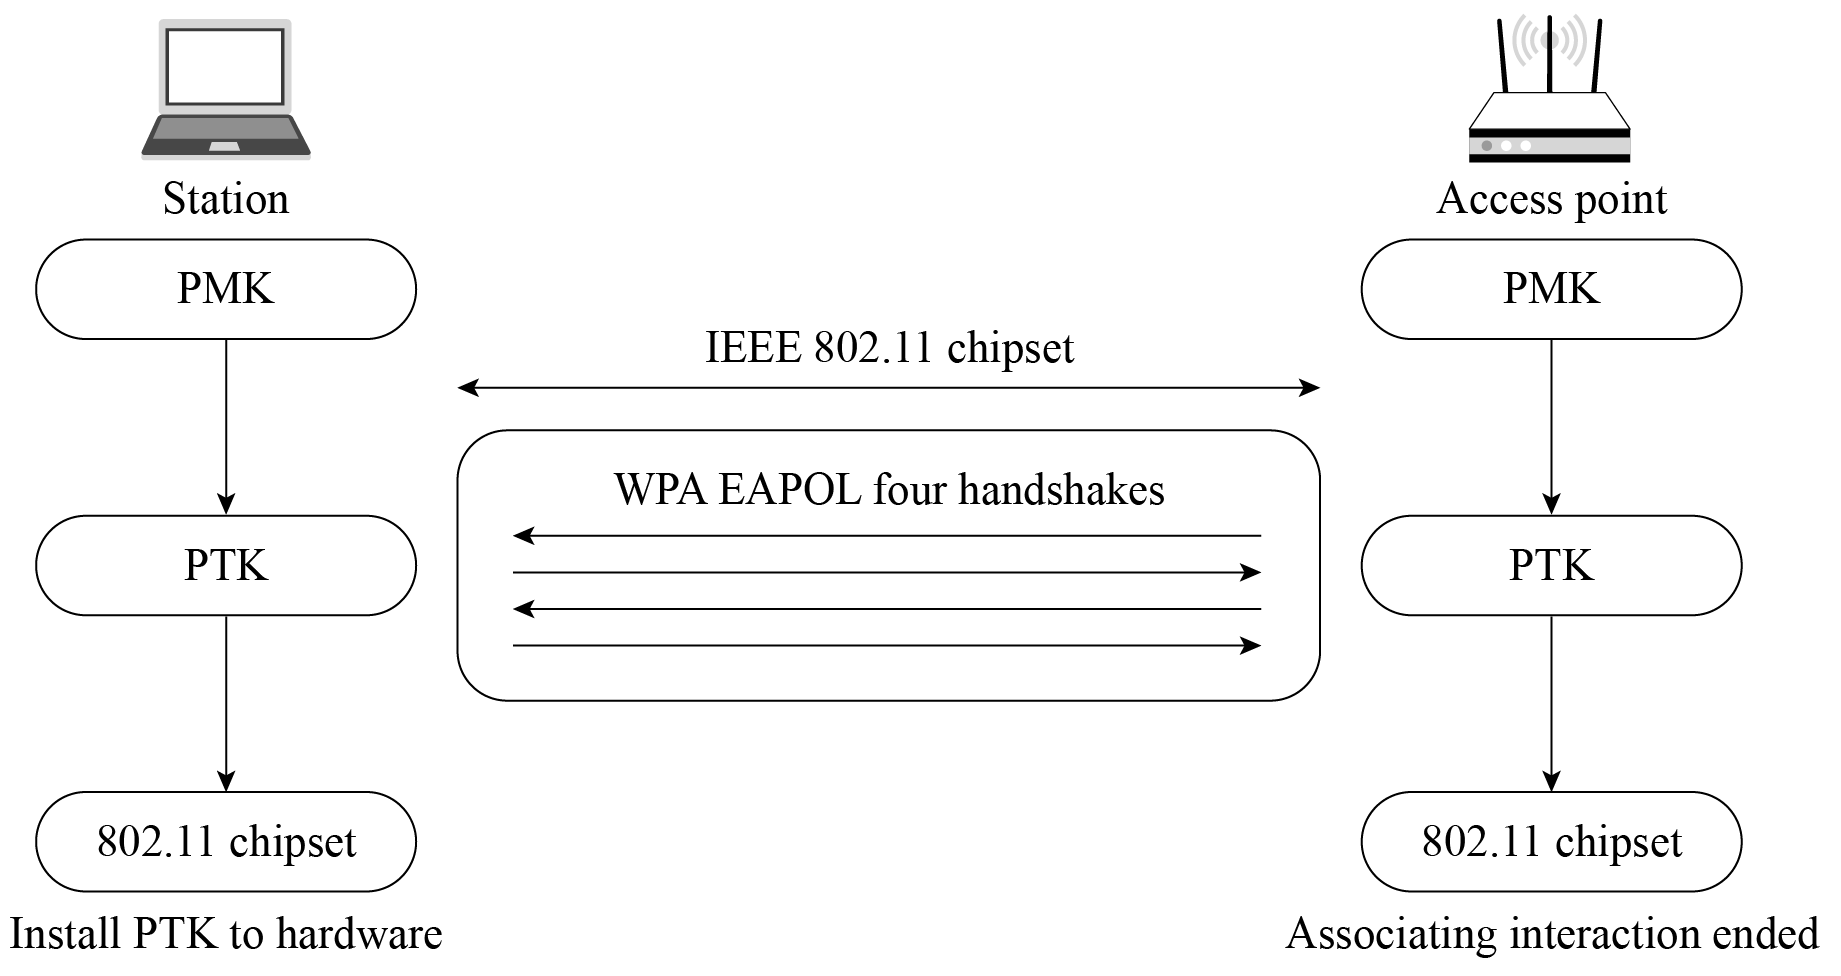
\includegraphics[width=0.65\textwidth]{D7Z/7-9}
        \caption{Generation of PMK from PSK}
    \end{figure}
    
    In WPA2-PSK, PMK is identical with PSK. But in WPA3, it generates new PMK through the SAE method based on the PMK from WPA2, to ensure that every STA has a unique PMK at different stages. Figure 7.10 shows how PMK is generated through SAE.

    \begin{figure}[!h]
        \centering
        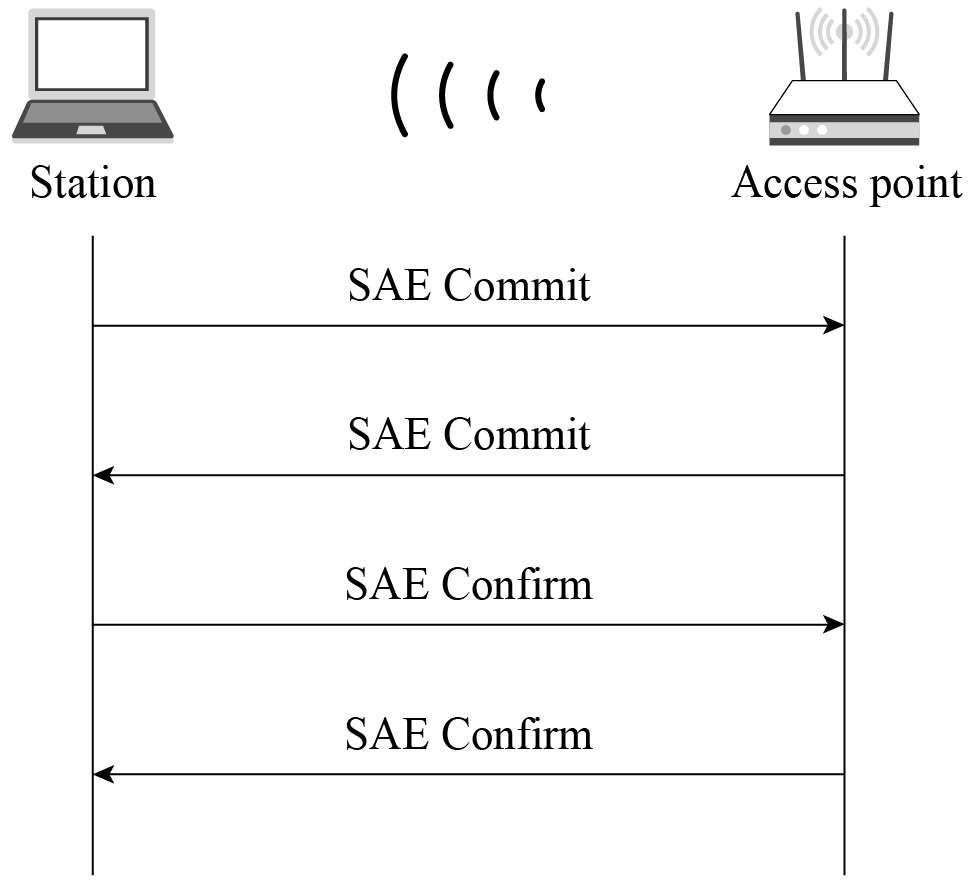
\includegraphics[width=0.4\textwidth]{D7Z/7-10}
        \caption{Generation of PMK with SAE}
    \end{figure}

    SAE treats the Supplicant and the Authenticator as peers. Either of them can initiate authentication. The two parties exchange data with each other to prove their knowledge of the key and generate PMK. SAE includes two phases, Commit and Confirm. In the Commit phase, both parties send SAE Commit frames for deducing the PSK. Then in the Confirm phase, they send SAE Confirm frames to verify the PSK. Once verification succeeds, PMK will be generated and the association will proceed.

    \textbf{\textbullet\ Commit}
        
    The sender uses the Hunting and Pecking algorithm to generate a Password Element (PWE) based on PSK and the MAC addresses of the sender and receiver. Then the scalar integer and element coordinates are generated by the sender based on PWE and a random value through elliptic curve operation. Upon receiving the commit frame, the receiver verifies the frame, and uses both the local and received frame content to generate a Key Confirmation Key (KCK) and PMK. The KCK will generate and verify the frame content in the Confirm phase.

    \textbf{\textbullet\ Confirm}
        
    Both parties generate a verification code from the KCK, local and peer Scalars, and local and peer PWEs through the same hash algorithm. If the codes turn out to be identical, the verification passes.
    
    After the STA and AP obtain PMK, they will start key derivation. During this process, the AP and different STAs generate different keys, which are configured into hardware for encryption/decryption. Since the AP and STAs need to re-generate these keys every time they are associated, they are named Pairwise Transient Keys (PTK). AP and STA use the EAPOL-Key frame to exchange Nonce and other messages, when the Four-Way Handshake comes into play. The process is shown in Figure 7.11.

    \begin{figure}[!h]
        \centering
        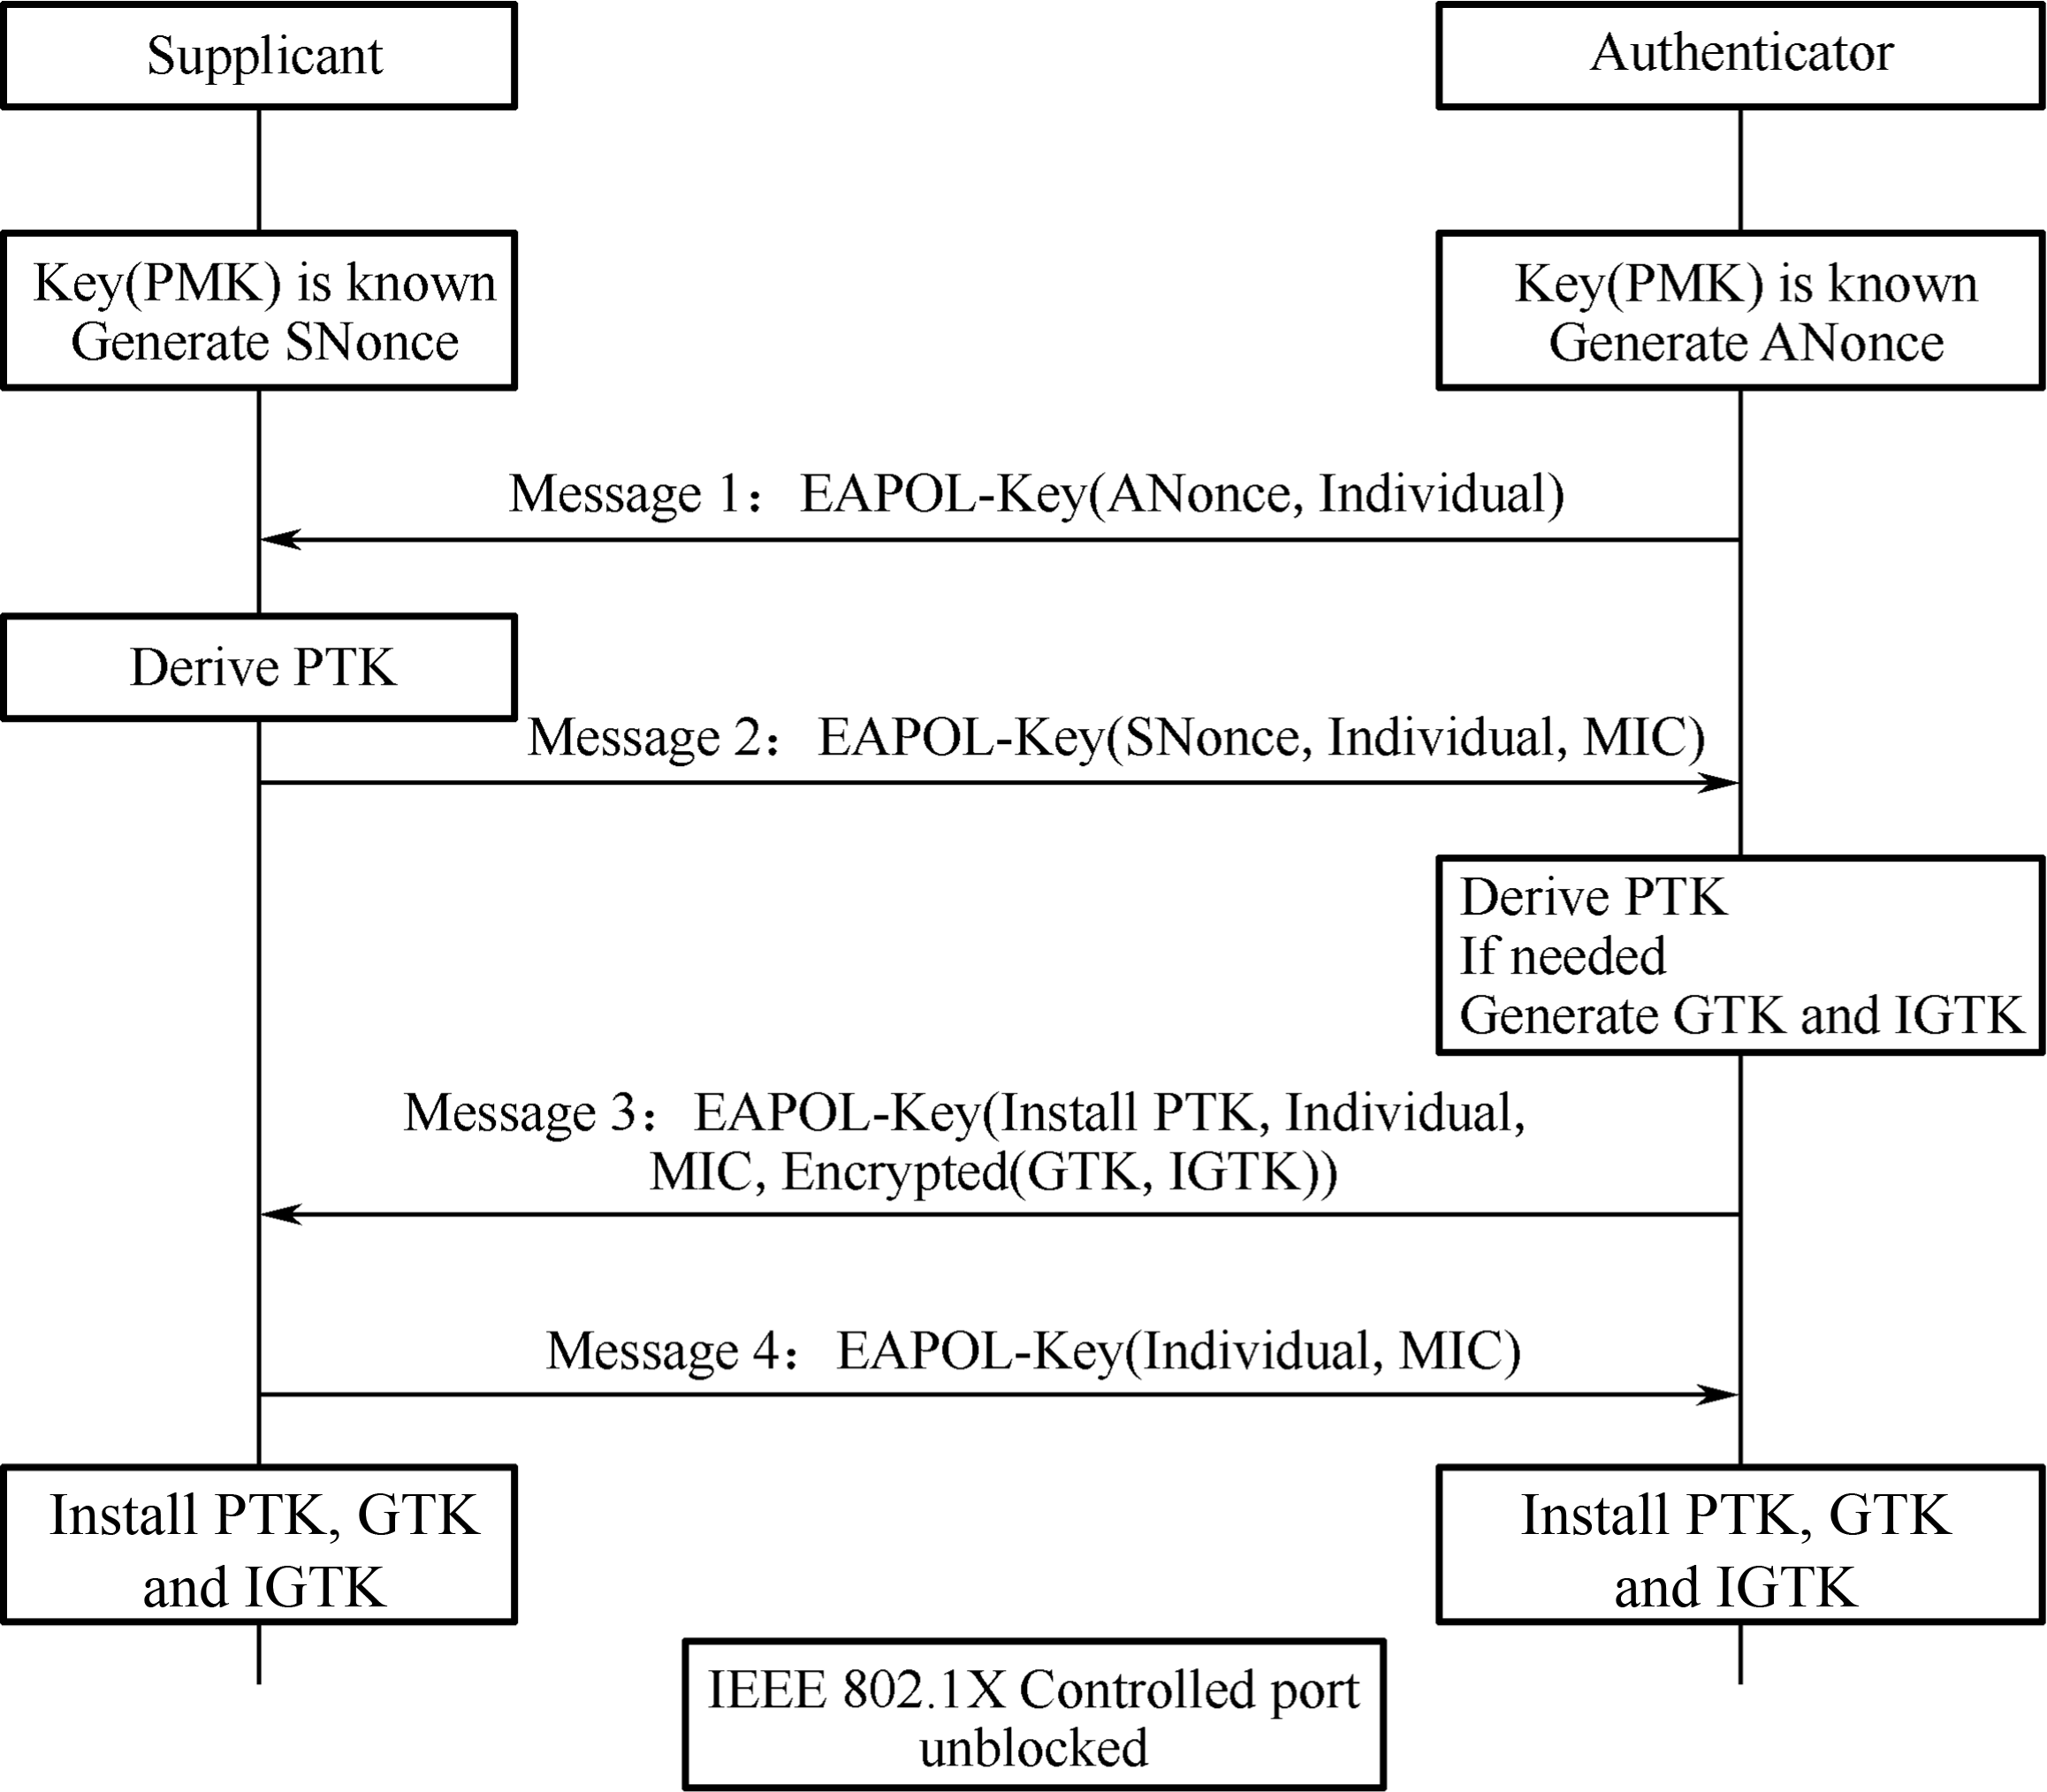
\includegraphics[width=0.58\textwidth]{D7Z/7-11}
        \caption{Process of Four-Way Handshake}
    \end{figure}

    \begin{enumerate}[label=(\arabic*)]
        \item The Authenticator generates a Nonce (ANonce), and sends it to the Supplicant in EAPOL-Key (Message 1).
        \item Supplicant performs key derivation based on the ANonce, its own Nonce (SNonce) and PMK, and Authenticator's MAC address . Then it sends the Authenticator another EAPOL-Key message (Message 2) that contains the SNonce. Message 2 also carries an MIC value encrypted by KCK. Once the Authenticator gets the SNonce in Message 2, it performs calculations similar to that of the Supplicant to verify whether the message returned is correct. If it is incorrect, which means the Supplicant’s PMK is wrong, the handshake will be terminated.
        \item If the Supplicant’s PMK is correct, the Authenticator will also perform key derivation. Later, the Authenticator sends the third EAPOL-Key message (Message 3) to the Supplicant. This message carries the Group Transient Key (GTK, used to update the group key encrypted by KEK) and MIC (encrypted by KCK). When the Supplicant receives Message 3, it will check whether the PMK of the AP is correct by calculation.
        \item The Supplicant sends the last EAPOL-Key message (Message 4) to the Authenticator for confirmation. Then both parties will use it to encrypt data.
    \end{enumerate}

    So far, the Supplicant and Authenticator have completed key derivation and pairing. They can eventually communicate with each other.
\end{term}

\section{Basics of Bluetooth}
This section will introduce Bluetooth from the following aspects:

\begin{itemize}
    \item What is Bluetooth?
    \item How does Bluetooth evolve?
    \item What do the Bluetooth concepts mean?
    \item How does Bluetooth connection work?
\end{itemize}

\subsection{Introduction to Bluetooth}
Bluetooth is a short-range wireless communication technology originally conceived by Ericsson in 1994. The goal of Bluetooth is to facilitate transmission and sharing of information over a short distance without cable connections among mobile devices, embedded devices, computer peripherals, and household appliances. Compared with other wireless communication technologies, Bluetooth boasts high security and easy connection.

\note[NOTE: Why “Bluetooth”?]{The word “Bluetooth” dates back more than a millennia to the Danish King Harald Bluetooth. King Harald is credited with the first unification of Scandinavia. Legend has it that King Harald liked blueberries so much that his teeth were stained blue. So he was called Bluetooth. In 1998, Intel, Nokia, Ericsson, and IBM established a Special Interest Group (SIG) called Bluetooth. The word Bluetooth quickly gained popularity and became synonymous with the short-range wireless communication technology.}

Bluetooth adopts decentralised network structure, fast frequency hopping, and short packet technology to support point-to-point and point-to-multipoint communication. It works in the 2.4 GHz ISM (Industrial, Scientific, Medical) band, which is commonly used worldwide. Bluetooth technology can be divided into two categories, Bluetooth Classic and Bluetooth Low Energy.

\begin{term}{Bluetooth Classic}
    Bluetooth Classic (BR/EDR) generally refers to modules that support the Bluetooth protocol below version 4.0, and are used for the transmission of large amounts of data such as voice and music. Bluetooth Classic protocols have different profiles of personal area networks for different scenarios. Commonly used profiles are Advanced Audio Distribution Profile (A2DP) for audio communication, Hands-Free Profile/Head-Set Profile (HFP/HSP) for hands-free devices, Serial Port Profile (SPP) for text serial port transparent transmission, and Human Interface Device (HID) for wireless input/output devices.
\end{term}

\begin{term}{Bluetooth Low Energy}
    Bluetooth Low Energy (LE) is a new type of ultra-low power wireless communication technology, designed for low-cost, less complicated wireless body and personal area networks. It is worth mentioning that Bluetooth LE chips can be powered by button cells. Together with microsensors, you can use the chips to build embedded or wearable sensors and applications of sensor networks.
\end{term}

In terms of protocols, Bluetooth 1.1, 1.2, 2.0, 2.1, and 3.0 apply to Bluetooth Classic, Bluetooth 4.0 supports both Bluetooth Classic and Bluetooth LE, and all later versions employ Bluetooth LE.

\subsection{Bluetooth Concepts}
This section introduces the network technologies related to Bluetooth, including the core architecture and components in Bluetooth specifications.

\begin{term}{Core architecture}
    The core system of Bluetooth is composed of Host, Controller, and Host Controller Interface (HCI). Host is used for application development, while Controller is for message sending and receiving, physical connection management, and other basic features which are implemented by dedicated Bluetooth chip manufacturers.

    \parskip 6pt
    The original design is to run the Host and the Controller independently on two chips or even systems, and they can communicate through the HCI. In this way, it is easier to replace and upgrade either module. Although there are many chips that put both the Host and the Controller together, they still follow this architecture, except that the HCI is changed from a hardware communication port to a software one.
    
    The Bluetooth LE protocol stack includes Physical Layer (PHY), Link Layer (LL), Logical Link Control and Adaptation Protocol (L2CAP), Attribute Protocol (ATT), Security Manager Protocol (SMP), Generic Attribute Profile (GATT), and Generic Access Profile (GAP), as shown in Figure 7.12.

    \begin{figure}[!h]
        \centering
        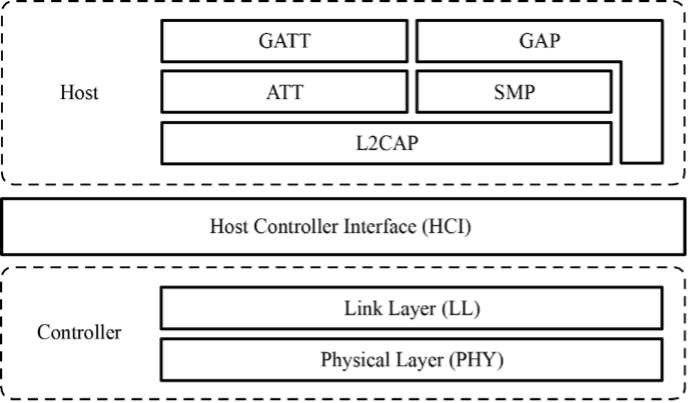
\includegraphics[width=0.6\textwidth]{D7Z/7-12}
        \caption{Protocol stack layers of Bluetooth LE}
    \end{figure}

    \begin{itemize}
        \item \textbf{Physical Layer (PHY)} specifies the wireless frequency band and modulation mode used by Bluetooth LE. How the PHY performs determines the power consumption, sensitivity, and selectivity of the Bluetooth LE chip and influences other radio frequency indicators.
        \item \textbf{Link Layer (LL)} only sends or receives data, leaving data analysis to GAP or ATT at the upper layer. LL is at the core of the Bluetooth LE protocol stack, as it decides which radio frequency channel to choose for communication, how to identify data packets transmitted through the air, when to send data packets, how to ensure data integrity, and how to manage and control links, how to receive and retransmit ACKs, etc.
        \item \textbf{Host Controller Interface (HCI)} provides a means of communication between the Host and the Controller. This layer can be implemented either by a hardware interface such as UART or USB in dual-chip architectures, or through a software API in single-chip architectures.
        \item \textbf{Logical Link Control and Adaptation Protocol (L2CAP)} provides connection-oriented and connectionless data services to upper layer protocols with protocol multiplexing capability, segmentation and reassembly operation, and group abstractions. It also permits per-channel flow control and retransmission.
        \item \textbf{Attribute Protocol (ATT)} defines data for user commands and command operations, such as reading or writing certain data. Bluetooth LE introduces the concept of attributes, which are used to describe data in a piece. Besides, ATT also defines the ATT commands that data can use. It is the layer that you will most frequently deal with.
        \item \textbf{Security Manager Protocol (SMP)} is responsible for the encryption and security of Bluetooth LE connections, without affecting user experience.
        \item \textbf{Generic Attribute Profile (GATT)} standardises the data content in attributes, and use the concept of groups to classify and manage attributes. Although the BLE protocol stack can operate without GATT, its interoperability will be compromised. It is GATT and a rich set of profiles that frees Bluetooth LE from the compatibility problem faced by other wireless protocols such as ZigBee.
        \item \textbf{Generic Access Profile (GAP)} defines effective data packets in LL, offering an easiest way to analyse LL payload. It is limited to features such as broadcasting, scanning, and initiating connections. 
    \end{itemize}
\end{term}

\begin{term}{Roles of Bluetooth}
    Bluetooth can be an Advertiser, a Scanner, or an Initiator. A master device plays the role of Initiator and Scanner, while a slave device plays the role of Advertiser.
    
    Bluetooth communication refers to the communication between two or more Bluetooth devices. It only occurs between masters and slaves, as slave devices cannot communicate directly.

    \parskip 6pt
    \begin{secterm}{Master mode}
        Master (or “central”) devices scan for slaves and initiate connection. In theory, if Bluetooth LE Mesh is not used to enable many-to-many device communication, only piconets can be established among devices.
        
        \parskip 6pt
        A device with Bluetooth technology can switch between master mode and slave mode. It normally works in slave mode and waits for master devices to connect. When needed, it switches to master mode and calls other devices. To initiate a call in master mode, a Bluetooth device needs to know the Bluetooth address and pairing password of the other device, and start calling after pairing successfully.
    \end{secterm}

    \begin{secterm}{Slave mode}
        Slave (or “peripheral”) devices advertise and wait for connections. Once connected, slaves can exchange data with the master.
    \end{secterm}

    In summary, a master can search for slaves and actively connects with them, while a slave cannot initiate any connection but to wait to be connected.
\end{term}

\begin{term}{Building Bluetooth networks}
    Now that we’ve learned about master and slave, let’s take a look at how to build Bluetooth networks. According to topological structures, Bluetooth networks can be divided into piconets, scatternets, and mesh networks.

    \parskip 6pt
    \begin{secterm}{Piconet}
        Every time a Bluetooth wireless link is formed, it is within a context of piconet. A piconet consists of two or more devices that occupy the same physical channel, which means the devices are synchronised according to a common clock and frequency hopping sequence. Figure 7.13 shows the piconet topology.

        \begin{figure}[!h]
            \centering
            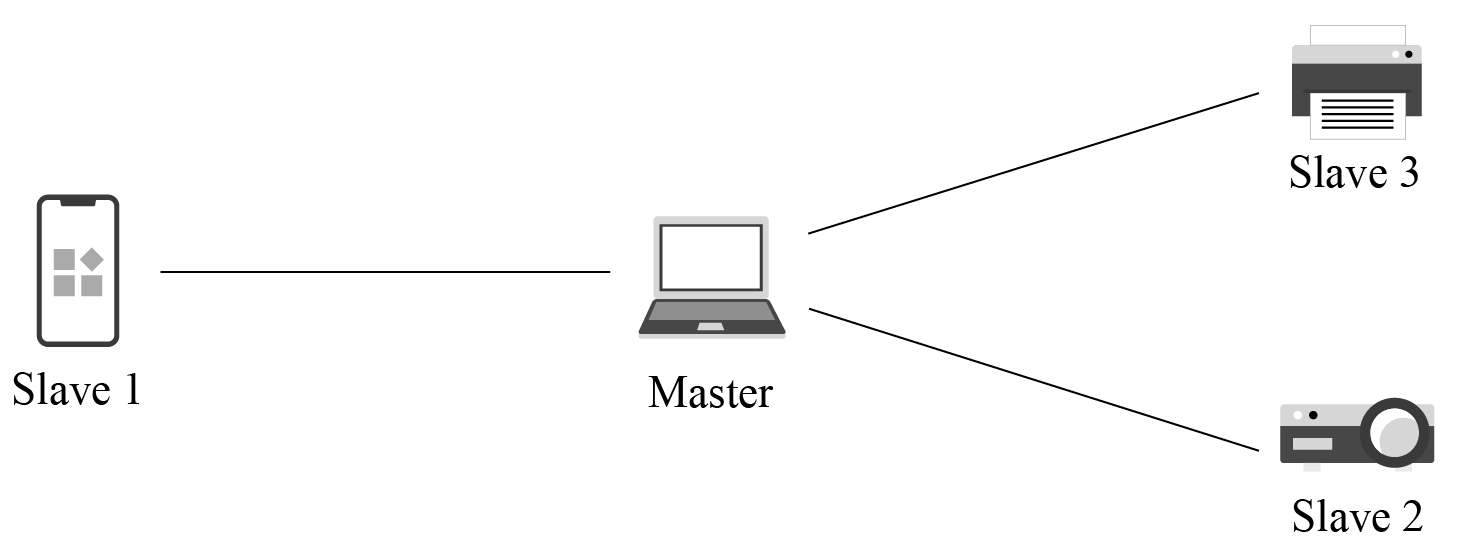
\includegraphics[width=0.6\textwidth]{D7Z/7-13}
            \caption{Piconet topology}
        \end{figure}
    \end{secterm}

    \begin{secterm}{Scatternet}
        A scatternet is formed when multiple piconets overlap. Figure 7.14 shows the scatternet topology.

        \vspace{6pt}
        Each piconet that constitutes a scatternet maintains its own master. The master of one piconet may act as the slave of another piconet at the same time. In Figure 7.14, the mobile phone is the master of the left piconet as well as the slave of the right piconet.

        \begin{figure}[!h]
            \centering
            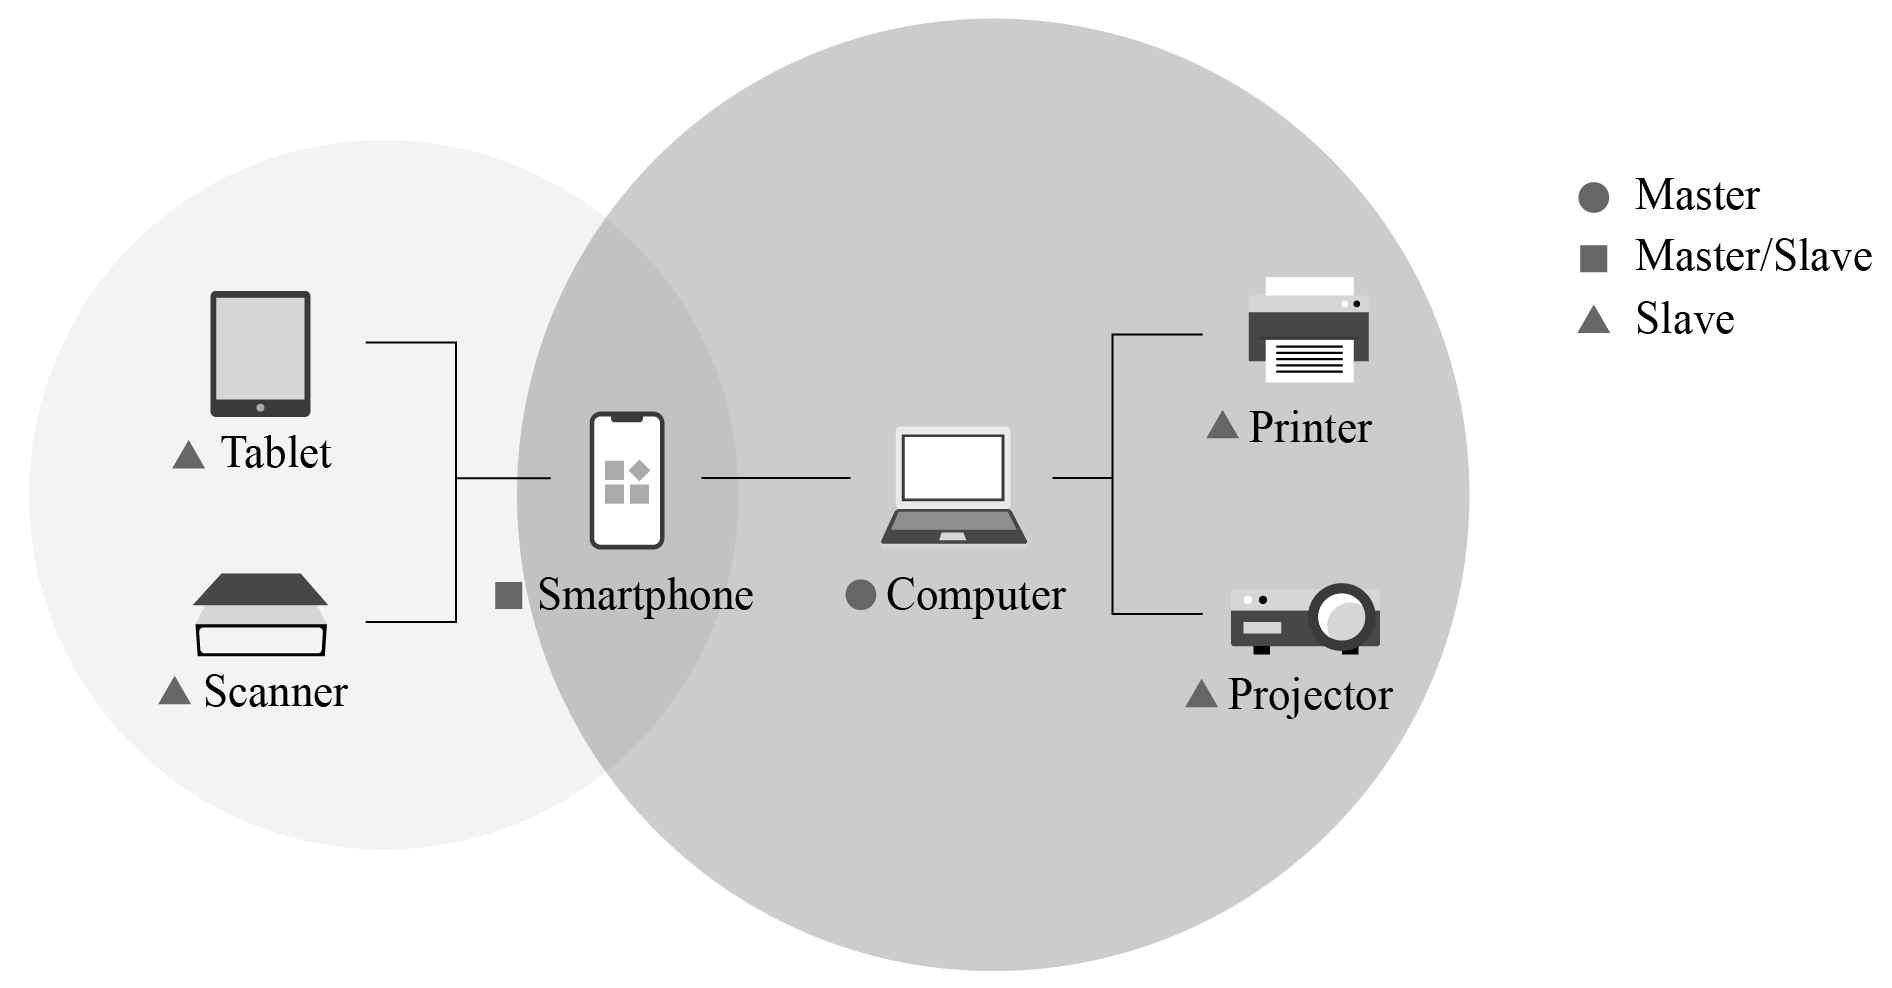
\includegraphics[width=0.8\textwidth]{D7Z/7-14}
            \caption{Scatternet topology}
        \end{figure}
    \end{secterm}

    \begin{secterm}{Mesh}
        Bluetooth Mesh was born after Bluetooth 4.0. It is a Bluetooth LE network used to establish many-to-many device communication. It allows the creation of large-scale networks, where dozens, hundreds, or even thousands of Bluetooth mesh devices can transmit data with each other. Bluetooth mesh is not the focus of this book, so you only need to know its definition for now.
    \end{secterm}
\end{term}

\subsection{Bluetooth Connection}
Bluetooth first searches for nearby devices through advertising or scanning, then establishes a connection, and finally form a network for data transmission.

\textbf{1. Slave advertising}

Usually, the peripheral device (slave) advertises itself and waits for the central device (master) to discover it and establish GATT connection for more exchange. In some cases, the peripheral only disseminates its own information to multiple central devices, without the need for connection.

To be discovered by a master, a slave will periodically send out advertising packets at an interval of \textit{t}. We call every advertising packet sent an “advertising event”, so \textit{t} is also called the advertising event interval, as shown in Figure 7.15.

\begin{figure}[!h]
    \centering
    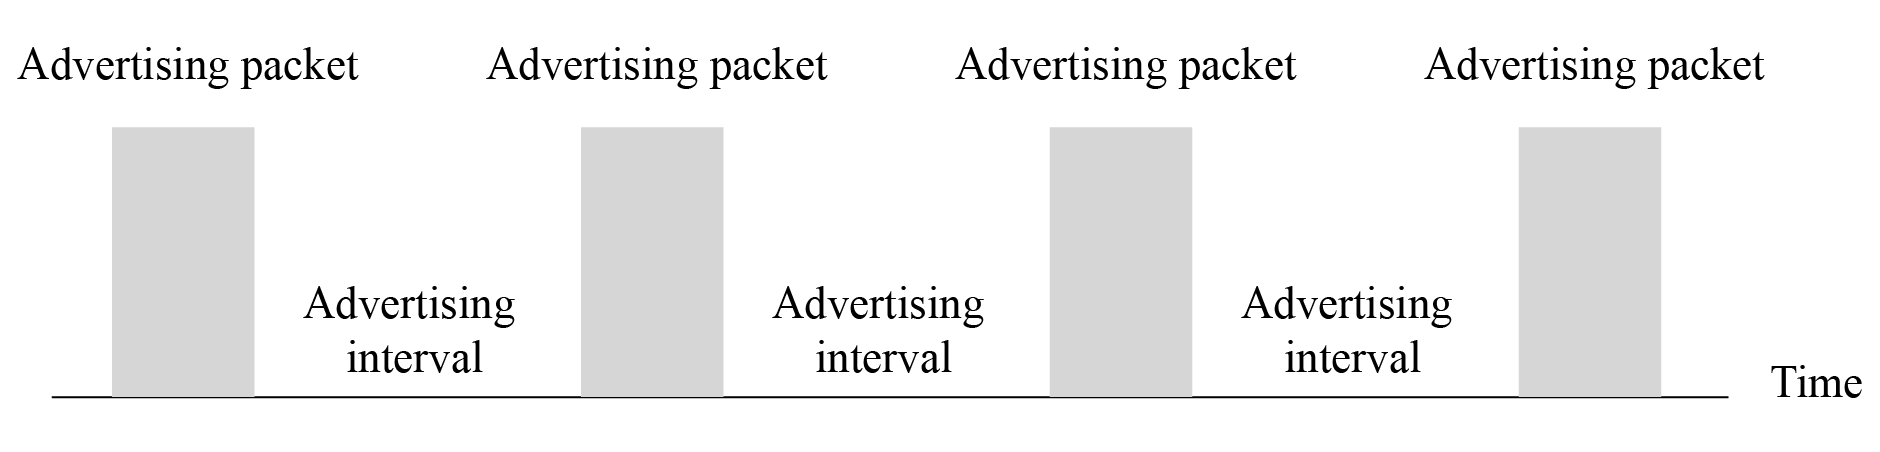
\includegraphics[width=0.85\textwidth]{D7Z/7-15}
    \caption{Slave advertising interval}
\end{figure}

Advertising events occur once in a while, and each event lasts for a period. The Bluetooth chip only enables the radio frequency module to send packets during the event, hence the relatively high power consumption. At other times, the chip goes idle, so the average power consumption is quite low.

Each advertising event contains three packets for the same message to be advertised on channel 37, 38, and 39 simultaneously. The process of slave advertising event is shown in Figure 7.16.

\begin{figure}[!h]
    \centering
    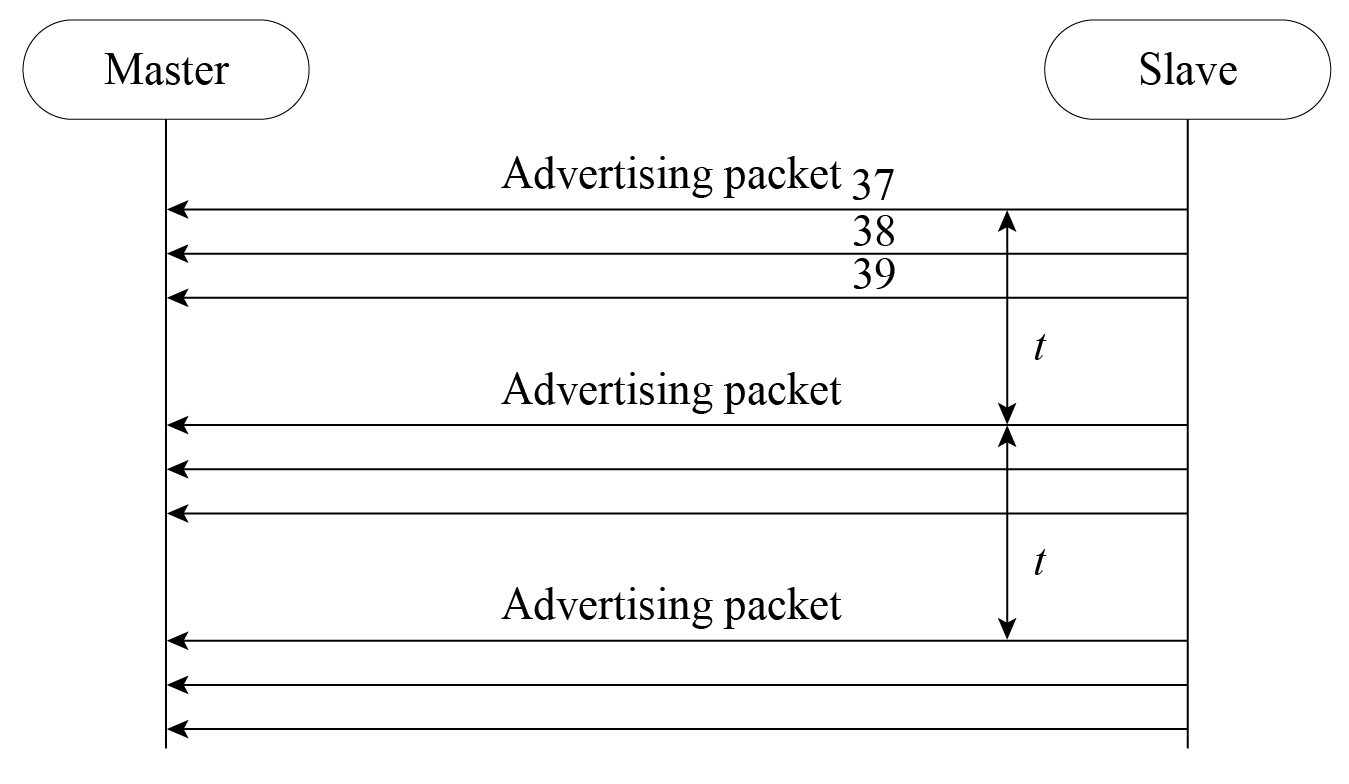
\includegraphics[width=0.6\textwidth]{D7Z/7-16}
    \caption{Slave advertising event}
\end{figure}

\textbf{2. Master scanning}

Scanning refers to the process when a master tries to find other Bluetooth LE devices within a certain range using advertising channels. Different from advertising, no interval or channel is set for scanning. The master may customise its own settings.

\begin{term}{Passive scanning}
    In passive scanning, the scanner only listens to advertising packets without sending any data to the advertiser., as shown in Figure 7.17.

    \begin{figure}[!h]
        \centering
        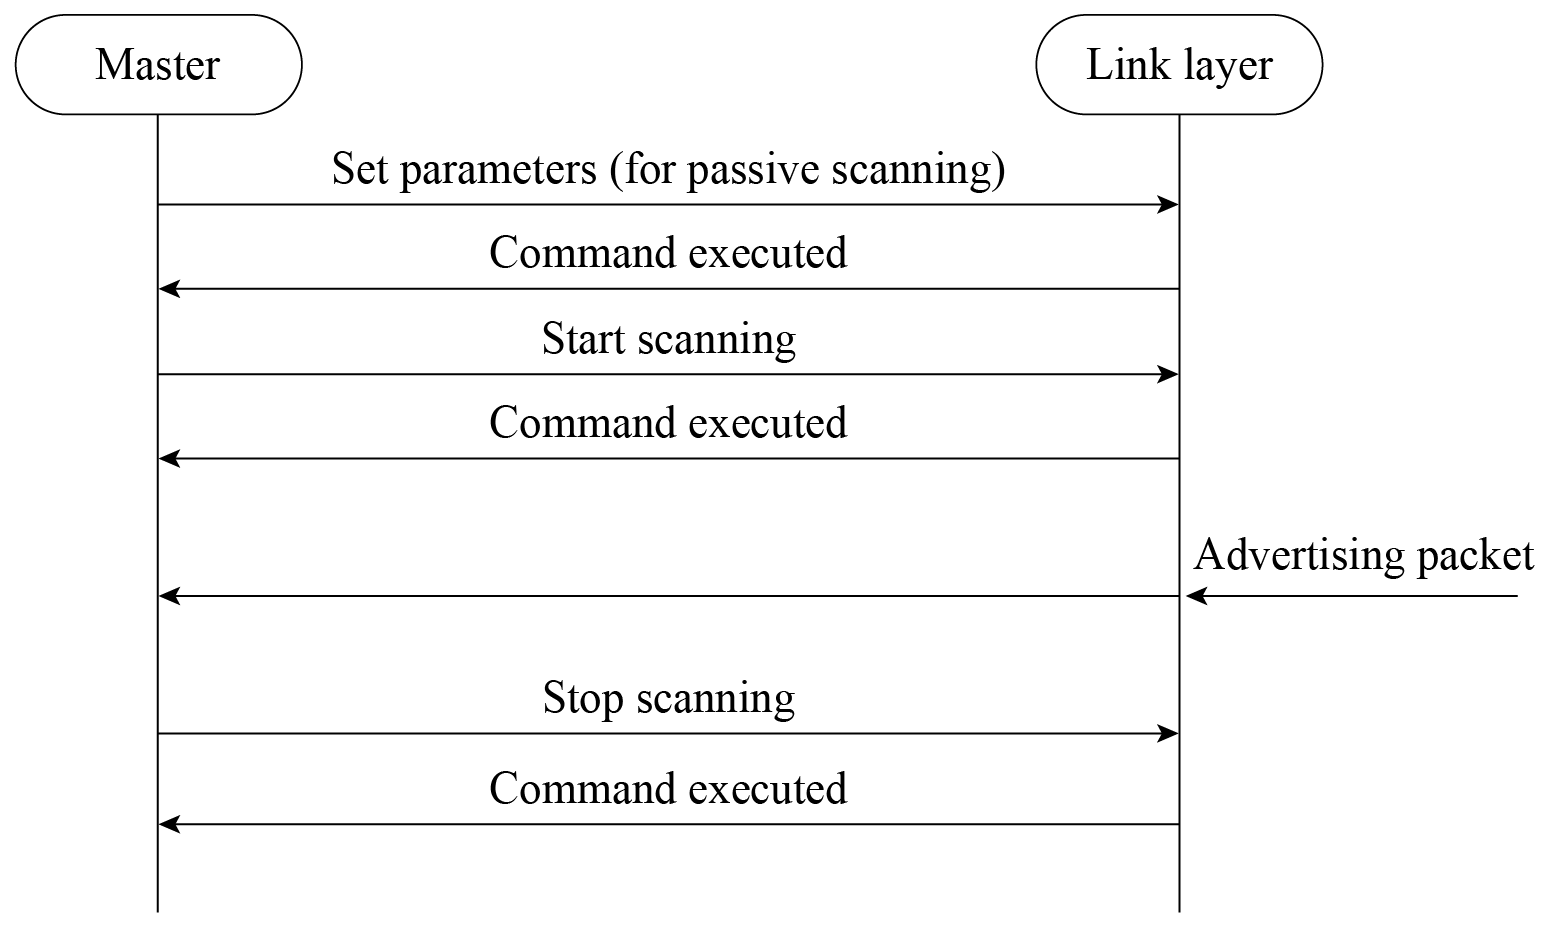
\includegraphics[width=0.65\textwidth]{D7Z/7-17}
        \caption{Passive scanning}
    \end{figure}

    \vspace{6pt}
    Once the scanning parameters are set, the master may send commands in the protocol stack to start scanning. During the process, if the controller receives an advertising packet that meets the filter policy or other constraints, it will report an event to the master. In addition to the advertiser’s address, the event also includes the data and the received signal strength indication (RSSI) of the advertising packet. Developers can estimate the signal path loss based on the RSSI and the transmission power of the advertising packet. This feature can be used to develop anti-lost trackers and positioning solutions.
\end{term}

\begin{term}{Active scanning}
     In active scanning, the master can capture not only the advertising packets sent by slaves but also the scan response packets, and distinguish the two types. See Figure 7.18 for the process of active scanning.

    \begin{figure}[!h]
        \centering
        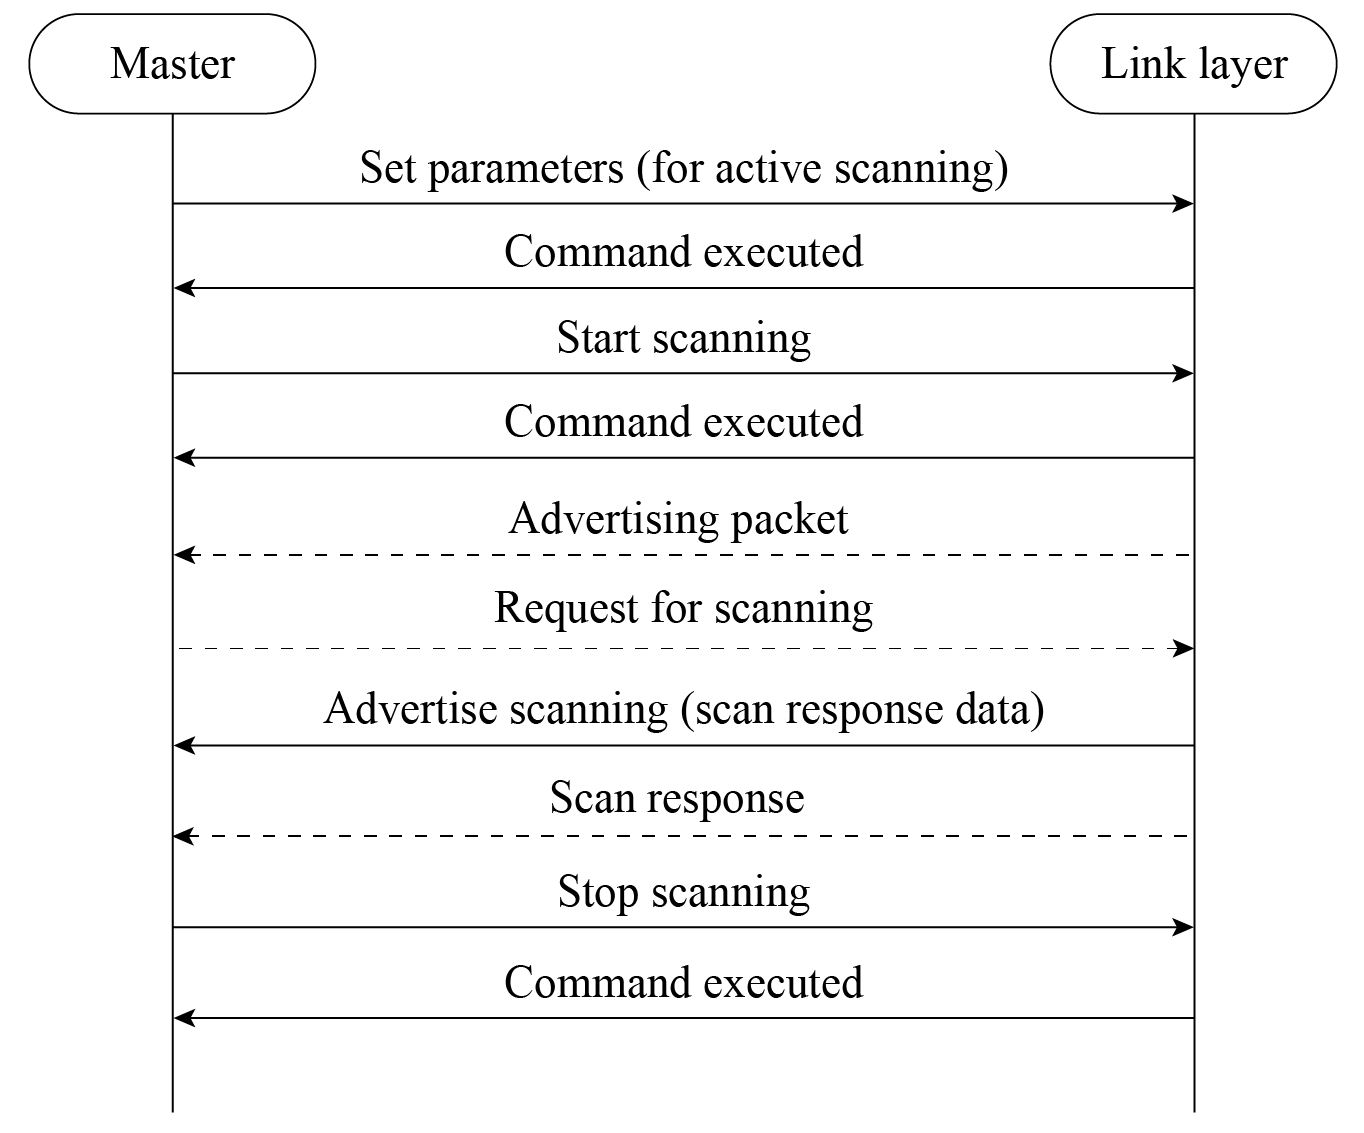
\includegraphics[width=0.6\textwidth]{D7Z/7-18}
        \caption{Active scanning}
    \end{figure}

    \vspace{6pt}
    After the controller receives any data, it will report an event to the master, containing the advertising type of the LL packet. The master can thereby decide whether to connect or scan the slave, and distinguish advertising packets from scan response packets.
\end{term}

\textbf{3. Master Connection}

\begin{enumerate}[label=(\arabic*)]
    \item The peripheral device starts advertising. Within the T\_IFS after sending an advertising packet, it enables radio frequency to receive packets from the central device. (T\_IFS: Inter Frame Space, the time interval between two packet transmissions on the same channel)
    \item The central device scans for advertising. Within the T\_IFS after receiving the advertising packet, if it enables scan response, it will reply to the peripheral device.
    \item Once the peripheral device receives scan response, it will return an ACK packet and prepare to receive data.
    \item If the central device does not receive the ACK packet, it will continue sending scan responses until it times out. During this period, only one ACK packet being received is enough to establish the connection.
    \item Now that the two devices are connected, they start communicating. The central device will send data packets to the peripheral at connection intervals, starting from the time when the advertising packet is received. The data packets are used to synchronise the clocks of the two devices and establish communication in master-slave mode. The process is as follows:

    \begin{enumerate}[label=\alph*., leftmargin=1.5em]
        \item Every time the peripheral device receives a packet from the central device, it resets the starting point to synchronise with the central device (service synchronsied with the client).
        \item Bluetooth LE communication is established in master-slave mode. The central device becomes the master, and the peripheral device becomes the slave. A slave can only send data back to the master within a specified time after the master sends a packet to it.
        \item Connection is established.
        \item The peripheral device automatically stops advertising, and it can no longer be found by other devices.
        \item During the interval between packet transmissions by the central device, the peripheral device may send multiple advertising packets.
    \end{enumerate}

    The communication sequence is shown in Figure 7.19.

    \begin{figure}[!h]
        \centering
        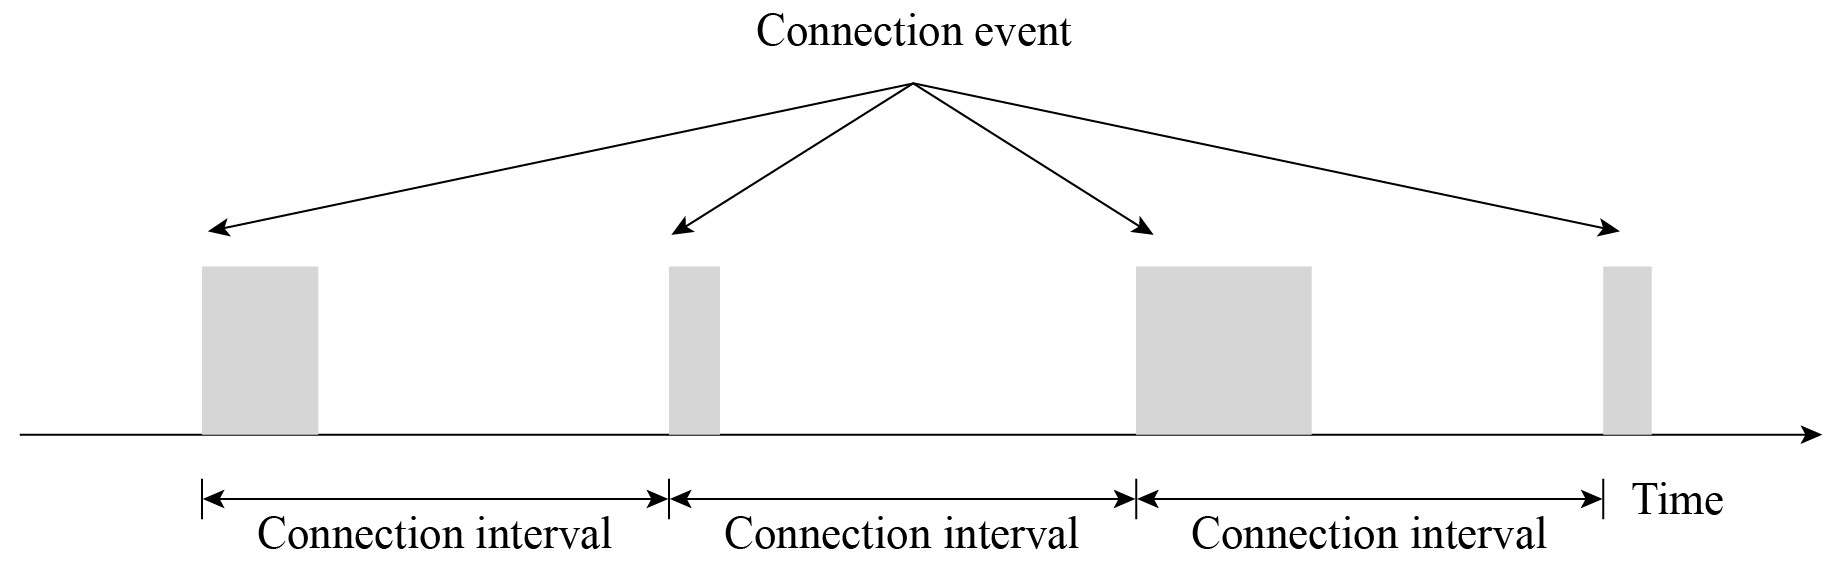
\includegraphics[width=0.9\textwidth]{D7Z/7-19}
        \caption{Communication sequence}
    \end{figure}
\end{enumerate}

To be disconnected, the central device only needs to stop sending packets. It can write the MAC address of the peripheral device into flash, SRAM, or other storage devices to keep monitoring the address, and reestablish communication when it receives advertising packets from the peripheral again. In order to save power, the slave will not send advertising packets if there is no data to be transmitted, and the two parties will be disconnected due to connection timeout. At this time, the central device needs to start monitoring, so that when the slave needs to send data, they can connect again.

\section{Wi-Fi Network Configuration}
With the development of IoT, more and more devices get connected via Internet. However, such devices do not have rich HCIs as smartphones and tablets. To connect them to the Internet, users cannot directly enter the SSID and password of the router. How to empower such devices, connecting them to the Internet or LANs using the router? This is one of the important targets of Wi-Fi devices. This section will cover some common network configuration methods.

\subsection{Wi-Fi Network Configuration Guide}
Network configuration is to provide SSID and password to Wi-Fi devices, so that they can connect to a specified AP and join its Wi-Fi network.

The final goal here is to send the SSID and password of the AP to the Wi-Fi device in different ways, and connect the device to the specified Wi-Fi network to join the LAN or Internet. Figure 7.20 shows the process of Wi-Fi network configuration.

\begin{figure}[!h]
    \centering
    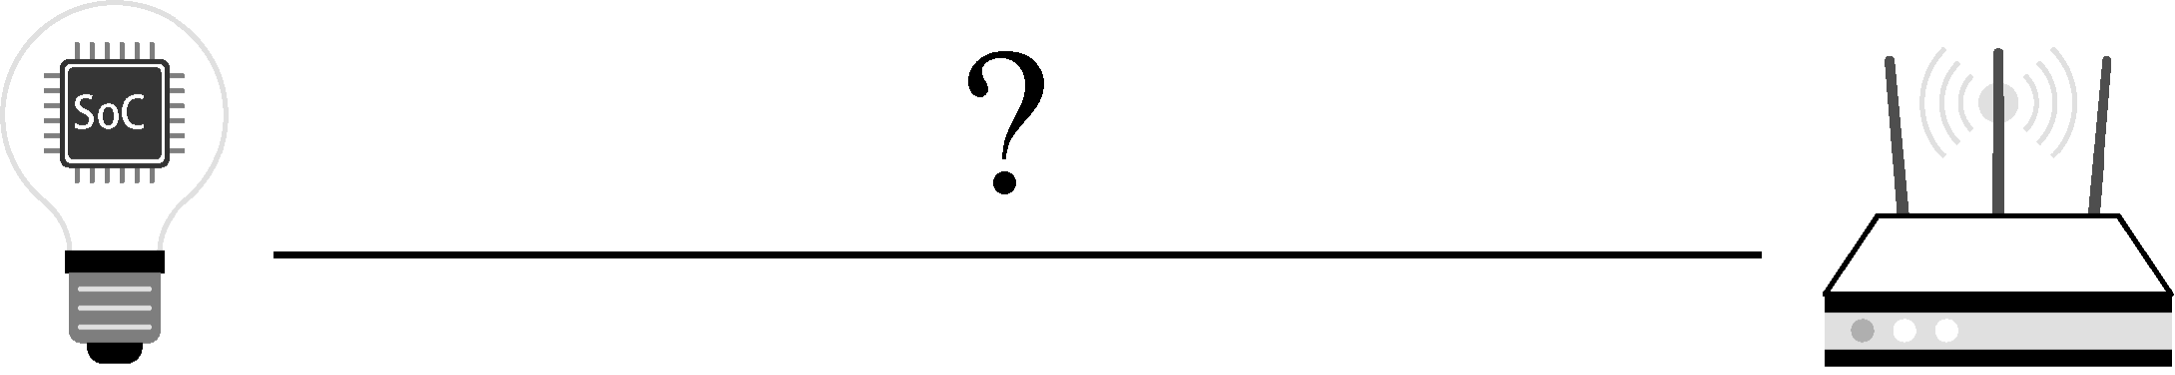
\includegraphics[width=0.5\textwidth]{D7Z/7-20}
    \caption{Process of Wi-Fi configuration}
\end{figure}

The IoT devices waiting for connection also need to be associated with an account, so here come some new concepts:

\begin{itemize}[noitemsep]
    \item \textbf{Network configuration in a narrow sense}: A Wi-Fi device obtains the AP information (SSID, password, etc.) and connects to the AP.
    \item \textbf{Binding}: Associating user's application accounts with the configured device.
    \item \textbf{Network configuration in a broad sense}: Network configuration in a narrow sense + binding.
\end{itemize}

This section will focus on network configuration in a narrow sense, thus omitting the binding process. At present, the most popular methods to configure networks are SoftAP, SmartConfig, and Bluetooth.

\subsection{SoftAP}
\textbf{1. Introduction}

SoftAP is a traditional method. First, the IoT device to be configured establishes an AP. The user connects a smartphone, tablet, or other devices with HCIs to this AP, and sends information about the network providing device. Then, the IoT device looks for the corresponding network and connects with it. Figure 7.21 shows the steps of SoftAP network configuration.

\begin{figure}[!h]
    \centering
    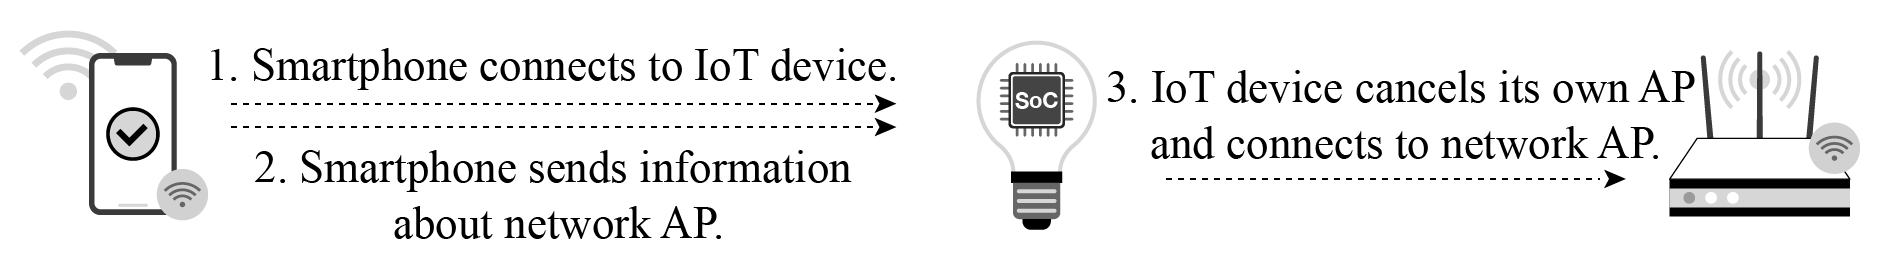
\includegraphics[width=0.8\textwidth]{D7Z/7-21}
    \caption{Steps of SoftAP network configuration}
\end{figure}

The SoftAP mechanism connects devices directly to the LAN without routers, thereby preventing router compatibility issues. This makes it easier to successfully configure the network compared with SmartConfig. But the downside is that there is an extra step for connection, as we need to manually switch to the IoT SoftAP in the Wi-Fi list. If we want to access cloud services, we still need a router. Some smartphones may automatically switch APs, but with iOS 11.0 or previous versions, we need to do the extra settings manually.

\textbf{2. Configuration}

Figure 7.22 indicates how to configure networks via SoftAP.

In-depth introduction to SoftAP will be given later together with Wi-Fi programming.

\subsection{SmartConfig}
\textbf{1. Introduction}

SmartConfig allows smartphones to fill the SSID and password in the unencrypted header of the MAC packet according to a certain encoding format, and send them in segments to the IoT device in multiple times by broadcasting and multicasting. Generally, we need to install an application on the smartphone for protocol interaction between the two parties. The steps of SmartConfig network configuration are shown in Figure 7.23.

After the receiver enables SmartConfig, the IoT device starts monitoring data on the router from channel 1. Once detecting data packets that meet the rules, it stops switching and stays on the current channel to receive all the data. Otherwise, the IoT device automatically switches to the subsequent channels until channel 13, and start over from channel 1.

The frame format of MAC layer in IEEE 802.11 allows for clear identification of LL payload data, which includes the header and data of the network layer. This makes it possible to immediately extract and calculate the length of the payload data as soon as the MAC frames are received. The payload data here is usually the password. Figure 7.24 shows the packet structure of SmartConfig network configuration.

\begin{figure}[!h]
    \centering
    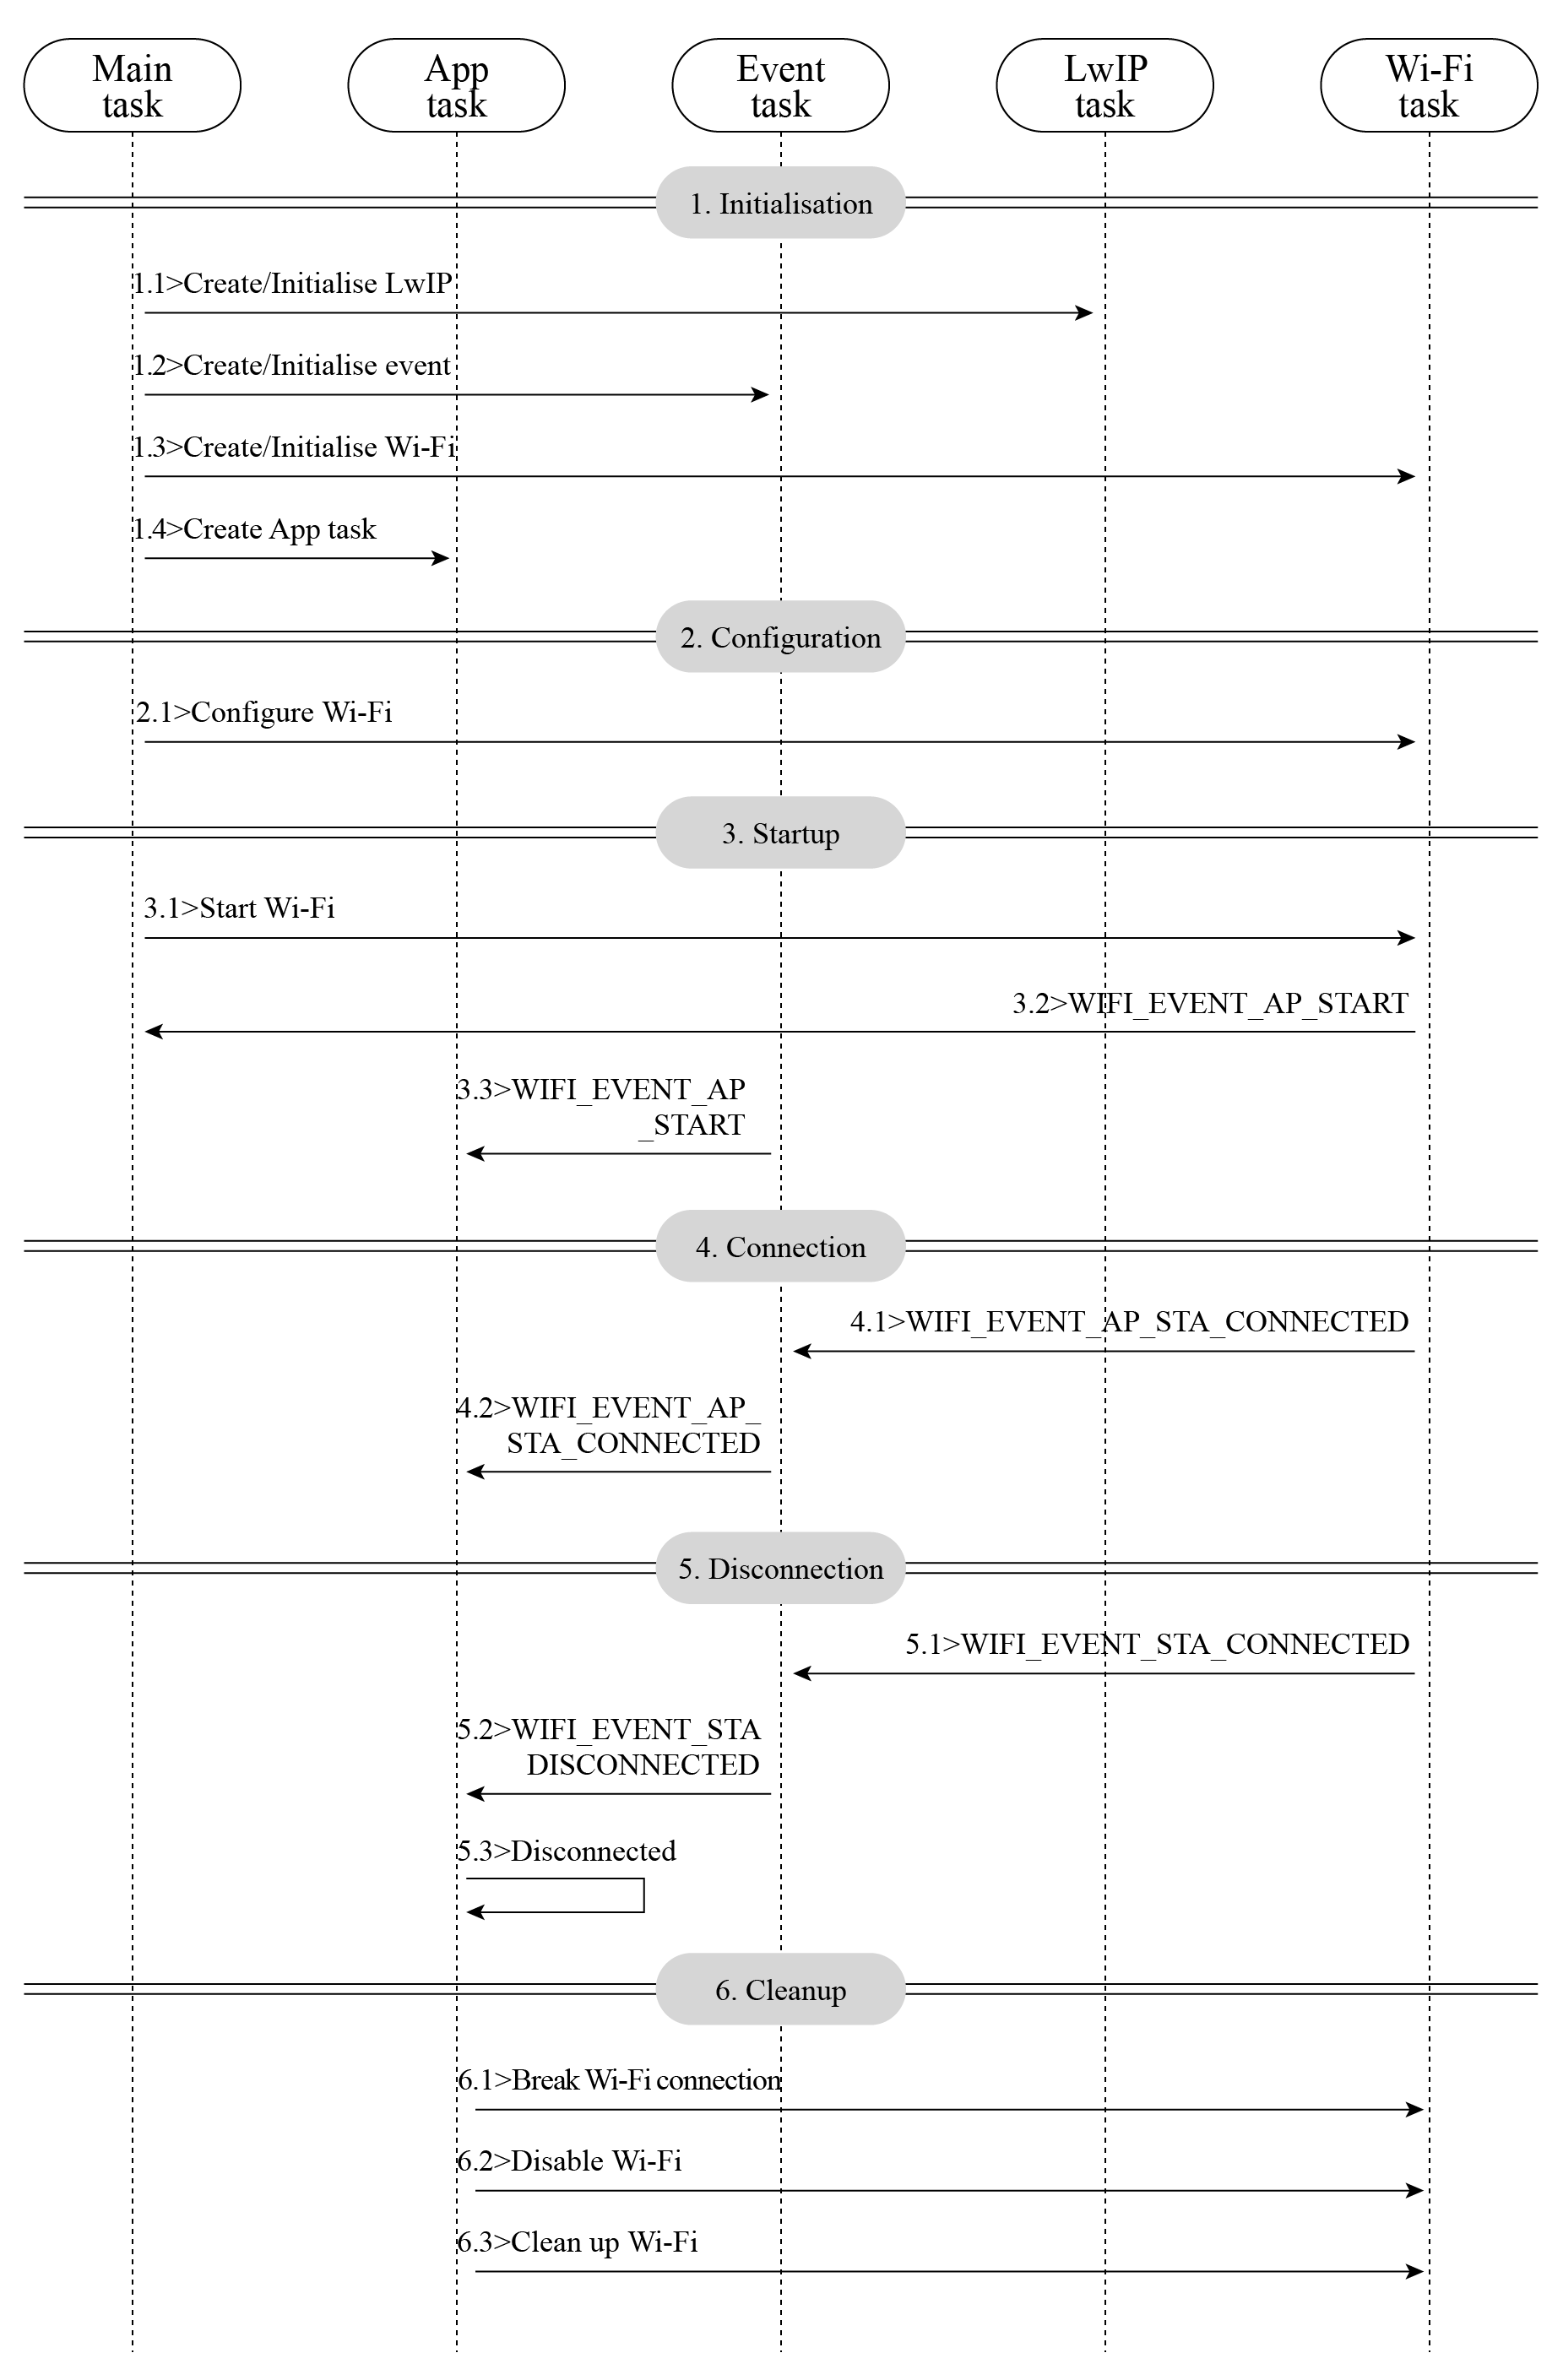
\includegraphics[width=0.82\textwidth]{D7Z/7-22}
    \caption{Network configuration via SoftAP}
\end{figure}

\begin{figure}[!h]
    \centering
    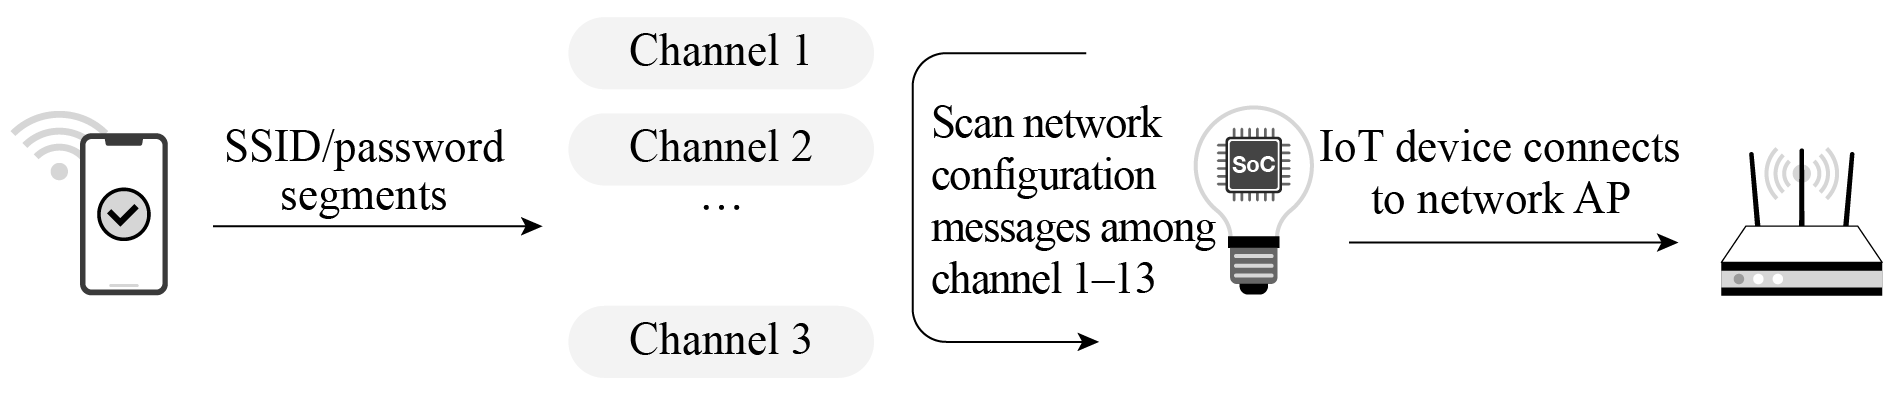
\includegraphics[width=0.8\textwidth]{D7Z/7-23}
    \caption{Steps of SmartConfig network configuration}
\end{figure}

\vspace{6pt}
\begin{figure}[!h]
    \centering
    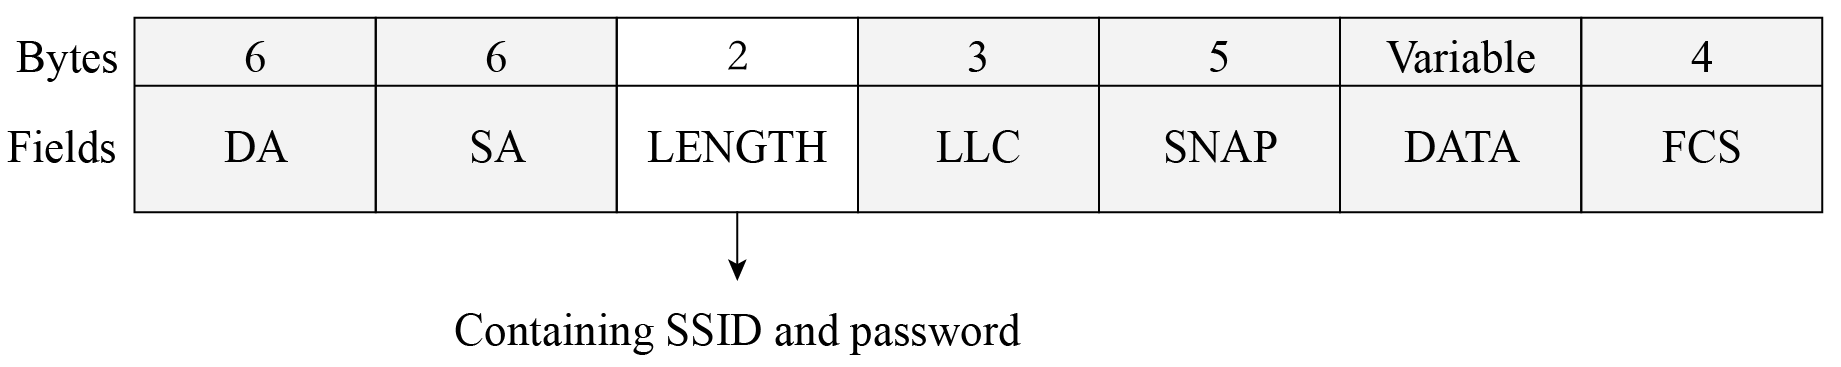
\includegraphics[width=0.85\textwidth]{D7Z/7-24}
    \caption{Packet structure of SmartConfig network configuration}
\end{figure}

Table 7.2 explains the fields of the data packet of SmartConfig network configuration.

\begin{table}[h!]
    \renewcommand{\arraystretch}{1.4}
    \caption{Fields of the data packet of SmartConfig network configuration}
    \begin{tabular}{|>{\Centering}m{0.25\textwidth}|>{\Centering}m{0.7\textwidth}|}
        \hline
        \rowcolor{LightBlue} \textbf{Data Frame}&\textbf{Description}\\
        \hline
        DA&Target MAC Address\\
        \hline
        SA&Source MAC Address\\
        \hline
        LENGTH&Payload Data Length\\
        \hline
        LLC&LLC Head\\
        \hline
        SNAP&3 B for Manufacturer Code and 2 B for Protocol Type\\
        \hline
        DATA&Payload Data\\
        \hline
        FCS&Frame Check Sequence\\
        \hline
    \end{tabular}
\end{table}

The sender usually uses the following methods to send data.

\begin{term}{UDP broadcasting}
    The MAC frame format of IEEE 802.11 ensures that the DA, SA, LENGTH, LLC, SNAP, and FCS fields are always visible to wireless signal monitors to acquire valid information, regardless of whether the channels are encrypted. When broadcasting, the sender is limited by the operating system, leaving only the LENGTH field at its disposal. However, by specifying a length-encoded communication protocol, a LENGTH field is enough for the sender to transmit the data needed.
\end{term}

\begin{term}{UDP multicasting}
    The multicast address is a reserved class D address, with a range of 224.0.0.0 to 239.255.\\255.255. The mapping between IP and MAC addresses is accomplished by setting the first 25 bits of the MAC address to 01.00.5E, while the last 23 bits of the MAC address corresponding to the bits of the IP address. As a result, the sender can encode data in the last 23 bits of the multicast IP and transmit it through the multicast packet for the receiver to decode.
\end{term}

SmartConfig offers user-friendly, smooth experience, but it places stringent requirements on the compatibility of smartphones and routers. For example, some routers may disable broadcast/multicast packet forwarding by default, preventing devices from receiving packets forwarded by the router. In other cases, different frequency bands used by smartphones and IoT devices can also result in configuration failure. If a smartphone is connected to a router using a 5 GHz frequency band, a device using the 2.4 GHz band may not be able to receive data. Such uncontrollable factors can significantly reduce overall compatibility and make it hard to successfully configure the network.

\textbf{2. Configuration}

The SmartConfig mechanisms developed by Espressif are:

\begin{itemize}
    \item \textbf{ESP-TOUCH V2}: UDP broadcast and multicast encoding.
    \parskip 0pt
    \item \textbf{ESP-TOUCH}: UDP broadcast encoding.
    \item \textbf{AIRKISS}: WeChat mini program.
\end{itemize}

\note[Source code]{In-depth introduction to SmartConfig will be given later together with Wi-Fi programming. Visit \url{https://github.com/espressif/esp-idf} to find the example code for \href{https://github.com/espressif/esp-idf/tree/master/examples/wifi/smart_config}{\texttt{examples/wifi/smart\_config}}.}

\subsection{Bluetooth}
\textbf{1. Introduction}

If the IoT device to be configured features Bluetooth, the network binding information can be sent via Bluetooth channel.

The principle behind the network configuration by Bluetooth is similar to that by SoftAP, except that the communication method used for transmitting Wi-Fi information is changed from Wi-Fi (AP mode) to Bluetooth. The IoT device to be configured creates a Bluetooth profile. The user then connects smartphones, tablets, or other devices with HCIs to it through a Bluetooth channel, and sends the information needed for network configuration. After receiving the information, the IoT device looks for corresponding AP and connects with it. The steps of Bluetooth network configuration are shown in Figure 7.25.

\begin{figure}[!h]
    \centering
    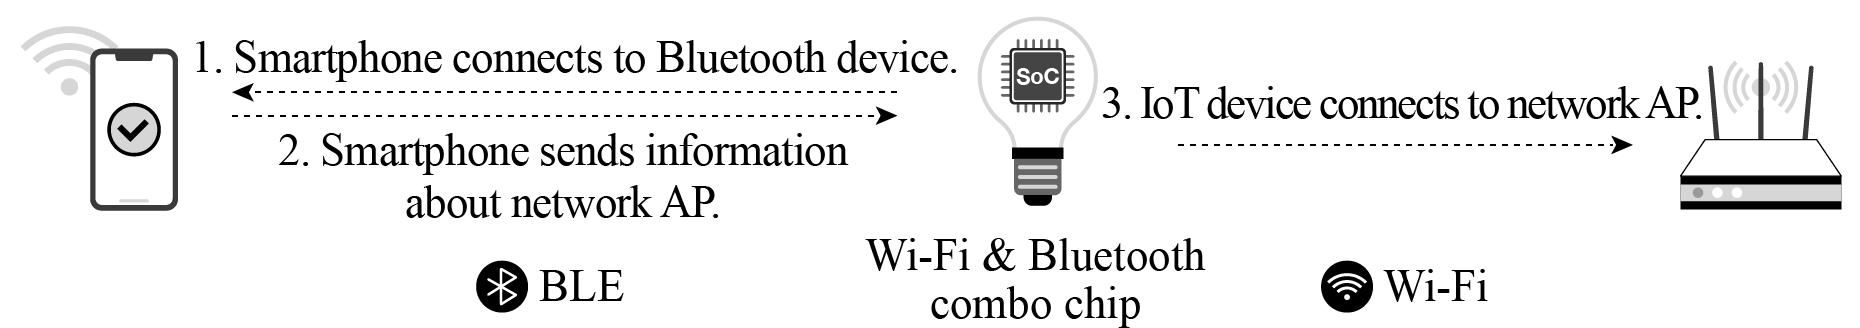
\includegraphics[width=0.8\textwidth]{D7Z/7-25}
    \caption{Steps of Bluetooth network configuration}
\end{figure}

The advantage of Bluetooth network configuration is that it eliminates the compatibility issues related to routers, producing higher connection rate. It can also discover and connect devices directly, so there is no need to turn on the device and connect to its own AP. However, the compatibility between the Bluetooth module and the mobile phone may affect network configuration. Additionally, using Bluetooth modules will increase the cost of the device.

\textbf{2. Configuration}

ESP32-C3 chip features both Wi-Fi and Bluetooth LE, thus supporting different network configuration methods. When it comes to Bluetooth network configuration, ESP32-C3 offers a comprehensive solution called BluFi. Figure 7.26 indicates how to configure networks via BluFi.

\begin{figure}[!h]
    \centering
    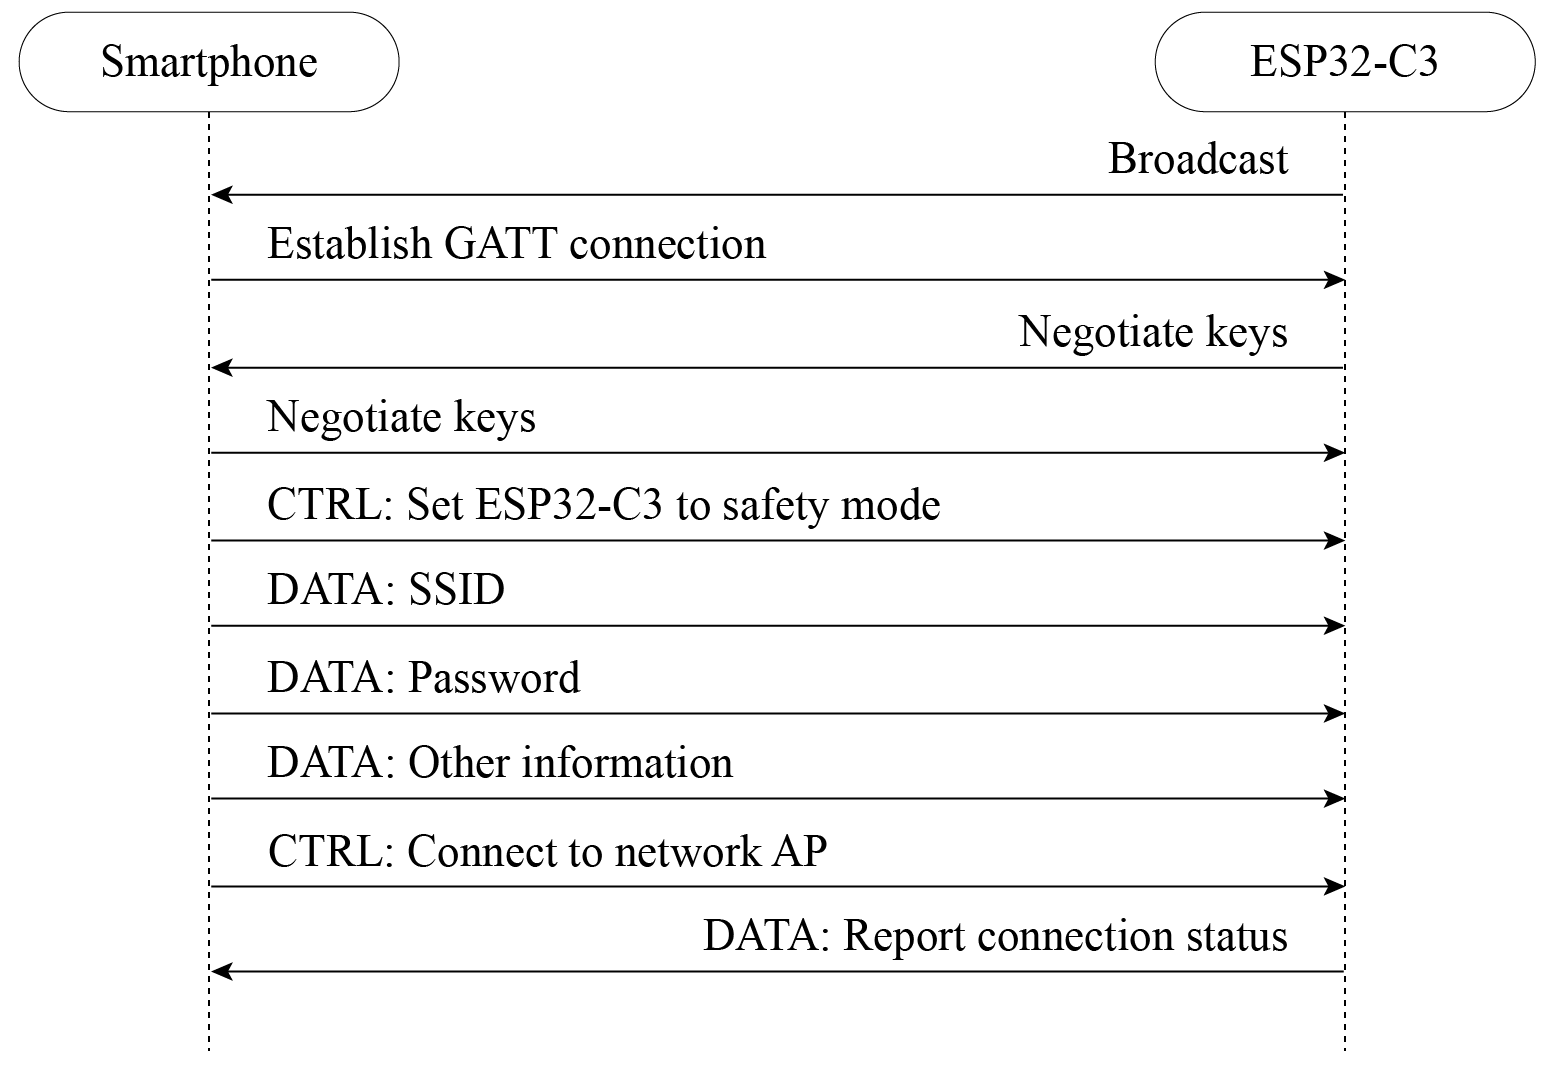
\includegraphics[width=0.7\textwidth]{D7Z/7-26}
    \caption{Network configuration via BluFi}
\end{figure}

\note[Source code]{In-depth introduction to Bluetooth network configuration will be given later together with Wi-Fi programming. Visit \url{https://github.com/espressif/esp-idf} to find the example code for \href{https://github.com/espressif/esp-idf/tree/master/examples/bluetooth/blufi}{\texttt{examples/bluetooth/blufi}}.}

\subsection{Other Methods}
\textbf{1. Direct network configuration}

Direct network configuration refers to sending SSID and password directly to IoT devices through peripheral interfaces such as UART, SPI, SDIO, and I2C according to a certain communication protocol. It is also known as wired network configuration. Once the IoT device receives the SSID and password, it connects to the AP and then returns the connection result through the master interface.

Moreover, some devices come with pre-set Wi-Fi information, such as SSID and password. When such devices are started in specified Wi-Fi environment, they can automatically connect to the corresponding AP. Such devices are typically used in large-scale networks, factory testing, or industrial scenarios. The steps of direct network configuration are shown in Figure 7.27.

\begin{figure}[!h]
    \centering
    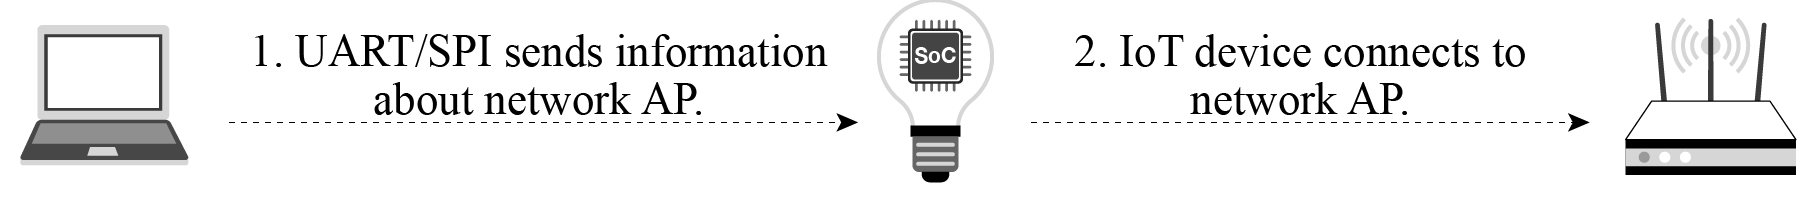
\includegraphics[width=0.8\textwidth]{D7Z/7-27}
    \caption{Steps of direct network configuration}
\end{figure}

This method adopts a software solution and is easy to implement. It is well-suited for devices with Wi-Fi chips or connected by transmission lines of other protocols. However, transmission lines must be pre-installed between systems.

The Espressif AT (ESP-AT) command firmware provided by Espressif can be directly used in mass-produced IoT applications. Developers can easily join wireless networks by running the Wi-Fi commands. For details, please refer to \href{https://docs.espressif.com/projects/esp-at/en/latest/esp32/index.html}{ESP-AT User Guide}.

\textbf{2. RouterConfig}

RouterConfig is based on Wi-Fi Protected Setup (WPS), a standard introduced by the Wi-Fi Alliance to address the complex process of configuring wireless network encryption and authentication settings. The goal of WPS is to simplify Wi-Fi security and network management for users. The standard offers two methods, Personal Identification Number (PIN) method and Push Button Configuration (PBC) method. Figure 7.28 shows the steps of RouterConfig.

\begin{figure}[!h]
    \centering
    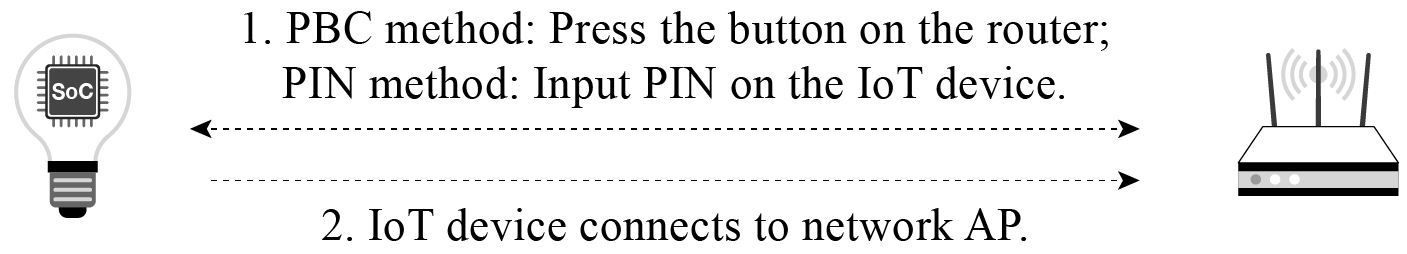
\includegraphics[width=0.7\textwidth]{D7Z/7-28}
    \caption{Steps of RouterConfig}
\end{figure}

The process is relatively straightforward, but it requires both the router and the device to support WPS. Unfortunately, many users neglect encryption security settings due to the cumbersome steps involved, which can lead to serious security issues. As a result, an increasing number of routers are abandoning or disabling support for WPS by default. The method has become less popular in recent years.

\note[Source code]{ESP-IDF, the official IoT development framework by Espressif, provides an example of this network configuration solution. The process there is quite simple. Visit \url{https://github.com/espressif/esp-idf} to see the example in \href{https://github.com/espressif/esp-idf/tree/master/examples/wifi/wps}{\texttt{examples/wifi/wps}}.}

\textbf{3. ZeroConfig}

ZeroConfig is a method of using one connected device to configure the network for another one. This method does not involve smartphones, as other devices like smart speakers can be used instead.

To initiate the process, the device to be connected sends its MAC address to the networked device through a custom message. The networked device then responds by sending back its saved router SSID and password via another custom message. After connecting, the device can perform further configuration such as external network binding. The steps of ZeroConfig network configuration are shown in Figure 7.29.

\begin{figure}[!h]
    \centering
    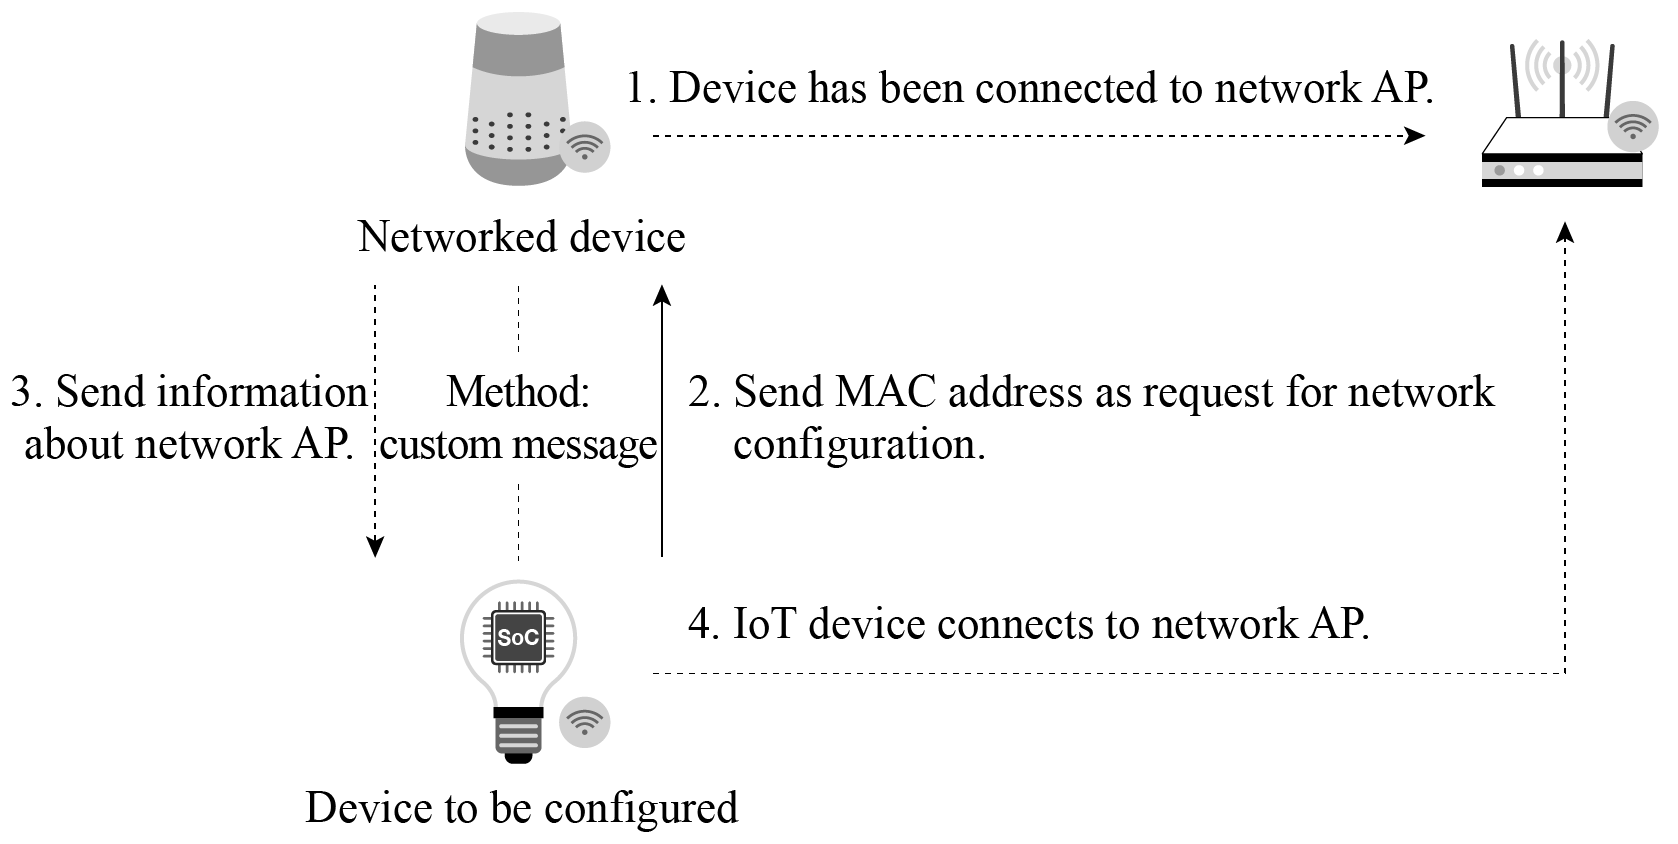
\includegraphics[width=0.7\textwidth]{D7Z/7-29}
    \caption{Steps of ZeroConfig}
\end{figure}

Since the networked device stores the SSID and password of the router, users do not need to enter them manually. The configuration will be easier, thus providing better user experience. However, this method cannot be widely adopted, as there must be networked devices connected with the router. At the same time, because mobile applications have limited access, it is impossible to assemble or receive Wi-Fi management frames through third-party programs. Therefore, smartphones can only be used to implement this method under certain circumstances.

\textbf{4. Phone AP network configuration}

Phone AP network configuration refers to setting a smartphone as an AP with a unique name and password, connecting the IoT device to the AP and sending network binding information. Figure 7.30 shows the steps of phone AP network configuration.

\begin{figure}[!h]
    \centering
    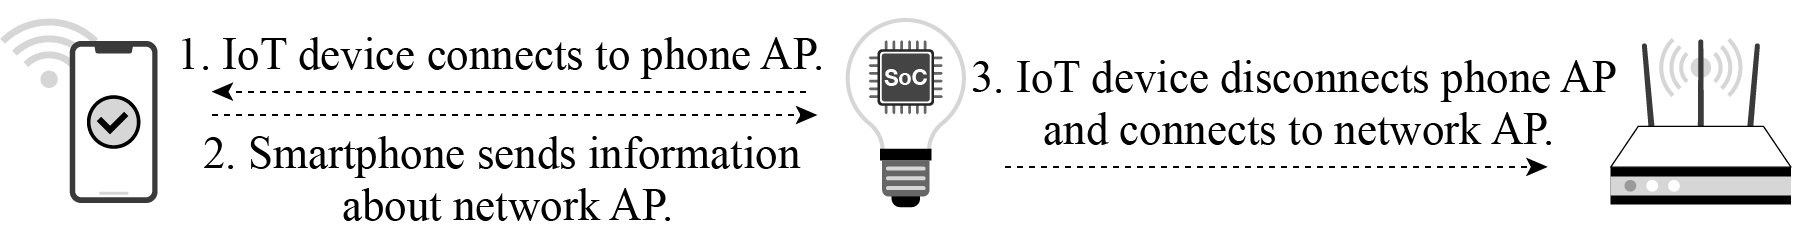
\includegraphics[width=0.8\textwidth]{D7Z/7-30}
    \caption{Steps of phone AP network configuration}
\end{figure}

Phone AP network configuration does not require the IoT device to support AP mode, so users do not have to do much development work on the device. It can be used with SmartConfig (simultaneously), making it a good candidate for backup network configuration. However, the user experience provided is barely satisfying. Many users struggle with setting the AP name of the smartphone or even enabling the phone AP. Particularly on iOS devices, the application cannot automatically create an AP, so users have to manually modify the device name and enable the AP. As a result, this method is not suitable for consumer devices.

In addition to the configuration methods above, Espressif also supports Wi-Fi Easy Connect, also known as Device Provisioning Protocol (DPP). For more information, please visit \url{https://bookc3/espressif.com/esp-dpp}.

\section{Wi-Fi Programming}
This section provides an overview of Wi-Fi APIs, covering how to use the APIs, to establish STA connection, and to connect in a smart way.

When developing a Wi-Fi application, the most efficient way is to adapt a similar example for your own requirements. Therefore, if you want to create a robust application, we suggest that you read this section and do the practices before getting started with your own project.

\subsection{Wi-Fi Components in ESP-IDF}
\textbf{1. Features}

Wi-Fi components can be used to configure and monitor the Wi-Fi network connection of ESP32-C3. The following features are supported.

\begin{itemize}[noitemsep]
    \item \textbf{STA mode}: aka station mode or Wi-Fi client mode. ESP32-C3 is connected to the AP in this mode.
    \item \textbf{AP mode}: aka SoftAP mode or access point mode. The AP is connected to ESP32-C3 in this mode.
    \item \textbf{AP-STA coexistence mode}: ESP32-C3 is connected to another AP as an AP.
    \item \textbf{Security standards} for the modes above: WPA, WPA2, WPA3, WEP, etc.
    \item \textbf{Scanning for APs}, including active and passive scanning.
    \item \textbf{Promiscuous mode} for monitoring IEEE 802.11 Wi-Fi packets.
\end{itemize}

\textbf{2. APIs}

\verb|esp_wifi.h| defines the APIs for Wi-Fi components, as shown in Table 7.3.

{\renewcommand{\arraystretch}{1.2}
\begin{longtable}{|>{\small}m{0.43\textwidth}|>{\small}m{0.55\textwidth}|}
    \caption{APIs for Wi-Fi components \label{7.3}} \\
        
    \hline
    \rowcolor{LightBlue}\multicolumn{1}{|c|}{\textbf{Function Name}}&\multicolumn{1}{c|}{\textbf{Description}}\\
    \hline
    \endfirsthead

    \multicolumn{2}{r}{Continuation of Table \ref{7.3}}\\
    \hline
    \rowcolor{LightBlue}\multicolumn{1}{|c|}{\textbf{Function Name}}&\multicolumn{1}{c|}{\textbf{Description}}\\
    \hline
    \endhead
        
    \verb|esp_wifi_init()|&Initialise resources for the Wi-Fi driver, such as Wi-Fi control structures and Wi-Fi tasks\\
    \hline
    \verb|esp_wifi_deinit()|&Free resources allocated in \verb|esp_wifi_init()| and stop Wi-Fi tasks\\
    \hline
    \verb|esp_wifi_set_mode()|&Set the WiFi operating mode for ESP32-C3\\
    \hline
    \verb|esp_wifi_get_mode()|&Get the WiFi operating mode of ESP32-C3\\
    \hline
    \verb|esp_wifi_start()|&Start Wi-Fi according to current configuration\\
    \hline
    \verb|esp_wifi_stop()|&Stop Wi-Fi according to current configuration\\
    \hline
    \verb|esp_wifi_connect()|&Connect ESP32-C3 to the AP\\
    \hline
    \verb|esp_wifi_disconnect()|&Disconnect ESP32-C3 from the AP\\
    \hline
    \verb|esp_wifi_scan_start()|&Scan for all available APs\\
    \hline
    \verb|esp_wifi_scan_stop()|&Stop the scan in progress\\
    \hline
    \verb|esp_wifi_scan_get_ap_num()|&Get the number of APs found by ESP32-C3\\
    \hline
    \verb|esp_wifi_scan_get_ap_records()|&Get the information about APs found by ESP32-C3\\
    \hline
    \verb|esp_wifi_set_config()|&Set the configuration of the ESP32-C3 STA or AP\\
    \hline
    \verb|esp_wifi_get_config()|&Get the configuration of the ESP32-C3 STA or AP\\
    \hline
\end{longtable}
}

\textbf{3. Programming model}

The ESP32-C3 Wi-Fi programming model is depicted in Figure 7.31.

\begin{figure}[!h]
    \centering
    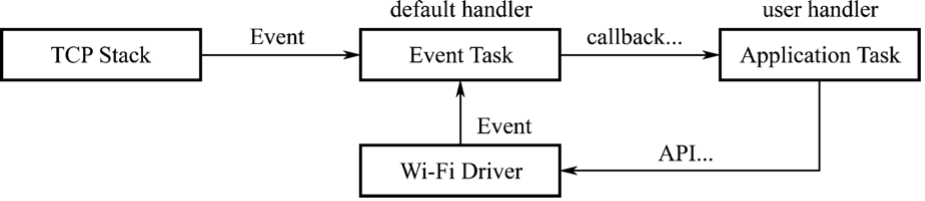
\includegraphics[width=0.8\textwidth]{D7Z/7-31}
    \caption{ESP32-C3 Wi-Fi programming model}
\end{figure}

The Wi-Fi driver can be considered a black box that knows nothing about upper-layer code, such as TCP stacks, application tasks, and event tasks. The application task (code) generally calls Wi-Fi driver APIs to initialise Wi-Fi and handles Wi-Fi events when necessary. The Wi-Fi driver receives API calls, handles them, and posts events in the application.

Wi-Fi event handling is based on the \verb|esp_event| library. Events are sent by the Wi-Fi driver to the default event loop. Applications may handle these events in callbacks registered using \verb|esp_event_handler_register()|. Wi-Fi events are also handled by the \verb|esp_netif| component to provide a set of default behaviors. For example, when a Wi-Fi station connects to an AP, \verb|esp_netif| will automatically start the Dynamic Host Configuration Protocol (DHCP) client by default.

\subsection{Exercise: Wi-Fi Connection}
\textbf{1. Put ESP32-C3 into STA mode, and connect to an AP.}

When operating in STA mode, ESP32-C3 can connect to an AP as an STA. 

The BSS based on the central AP allows for multiple STAs to build a wireless network, with the AP forwarding all communications within the network. In this mode, the device is able to access both the external and internal network directly, using the Internet Protocol (IP) address assigned by the AP. Figure 7.32 explains Wi-Fi STA mode.

\begin{figure}[!h]
    \centering
    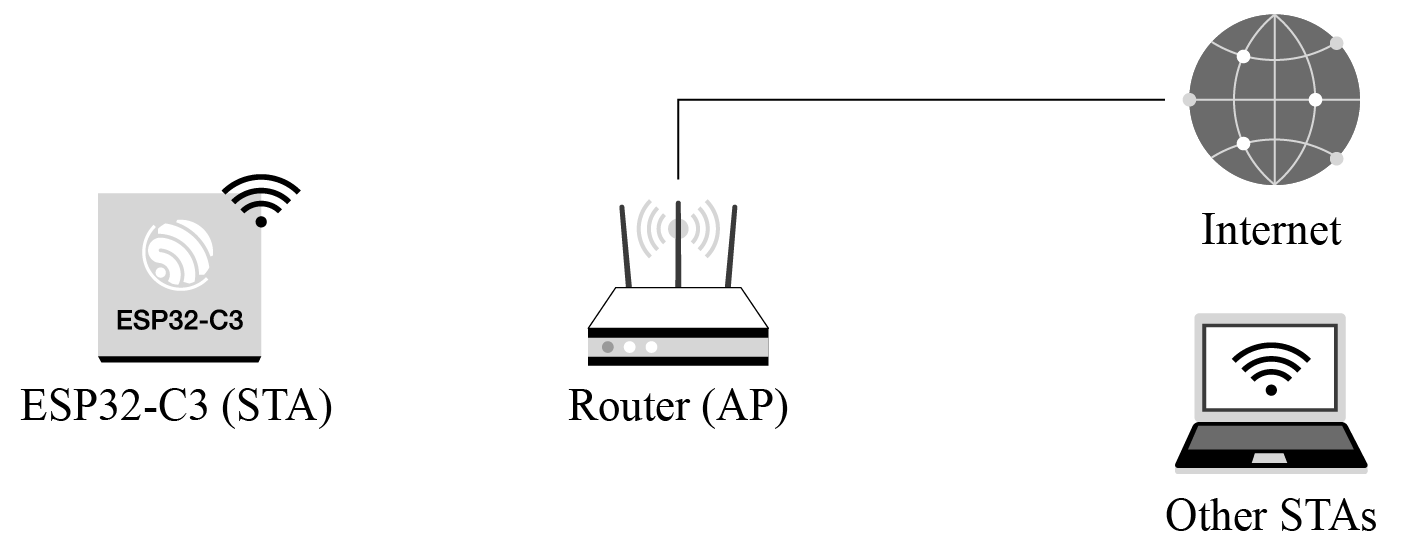
\includegraphics[width=0.65\textwidth]{D7Z/7-32}
    \caption{Wi-Fi STA mode}
\end{figure}

\textbf{2. Use ESP-IDF components to connect devices to routers.}

Figure 7.33 shows how to use ESP-IDF components to connect devices to routers.

(1) \textbf{Initialisation}. See 1.1, 1.2, and 1.3 in Figure 7.33.

a. \textbf{Initialise LwIP}. Create an LwIP core task and initialise LwIP-related work.
        
\begin{codebloc}
\begin{tabular}{d}
\verb|1.  ESP_ERROR_CHECK(esp_netif_init());|
\end{tabular}
\end{codebloc}

\newpage
\newgeometry{left=2cm,right=2cm,top=1.5cm,bottom=2cm} % set new margins
\begin{figure}[!h]
    \centering
    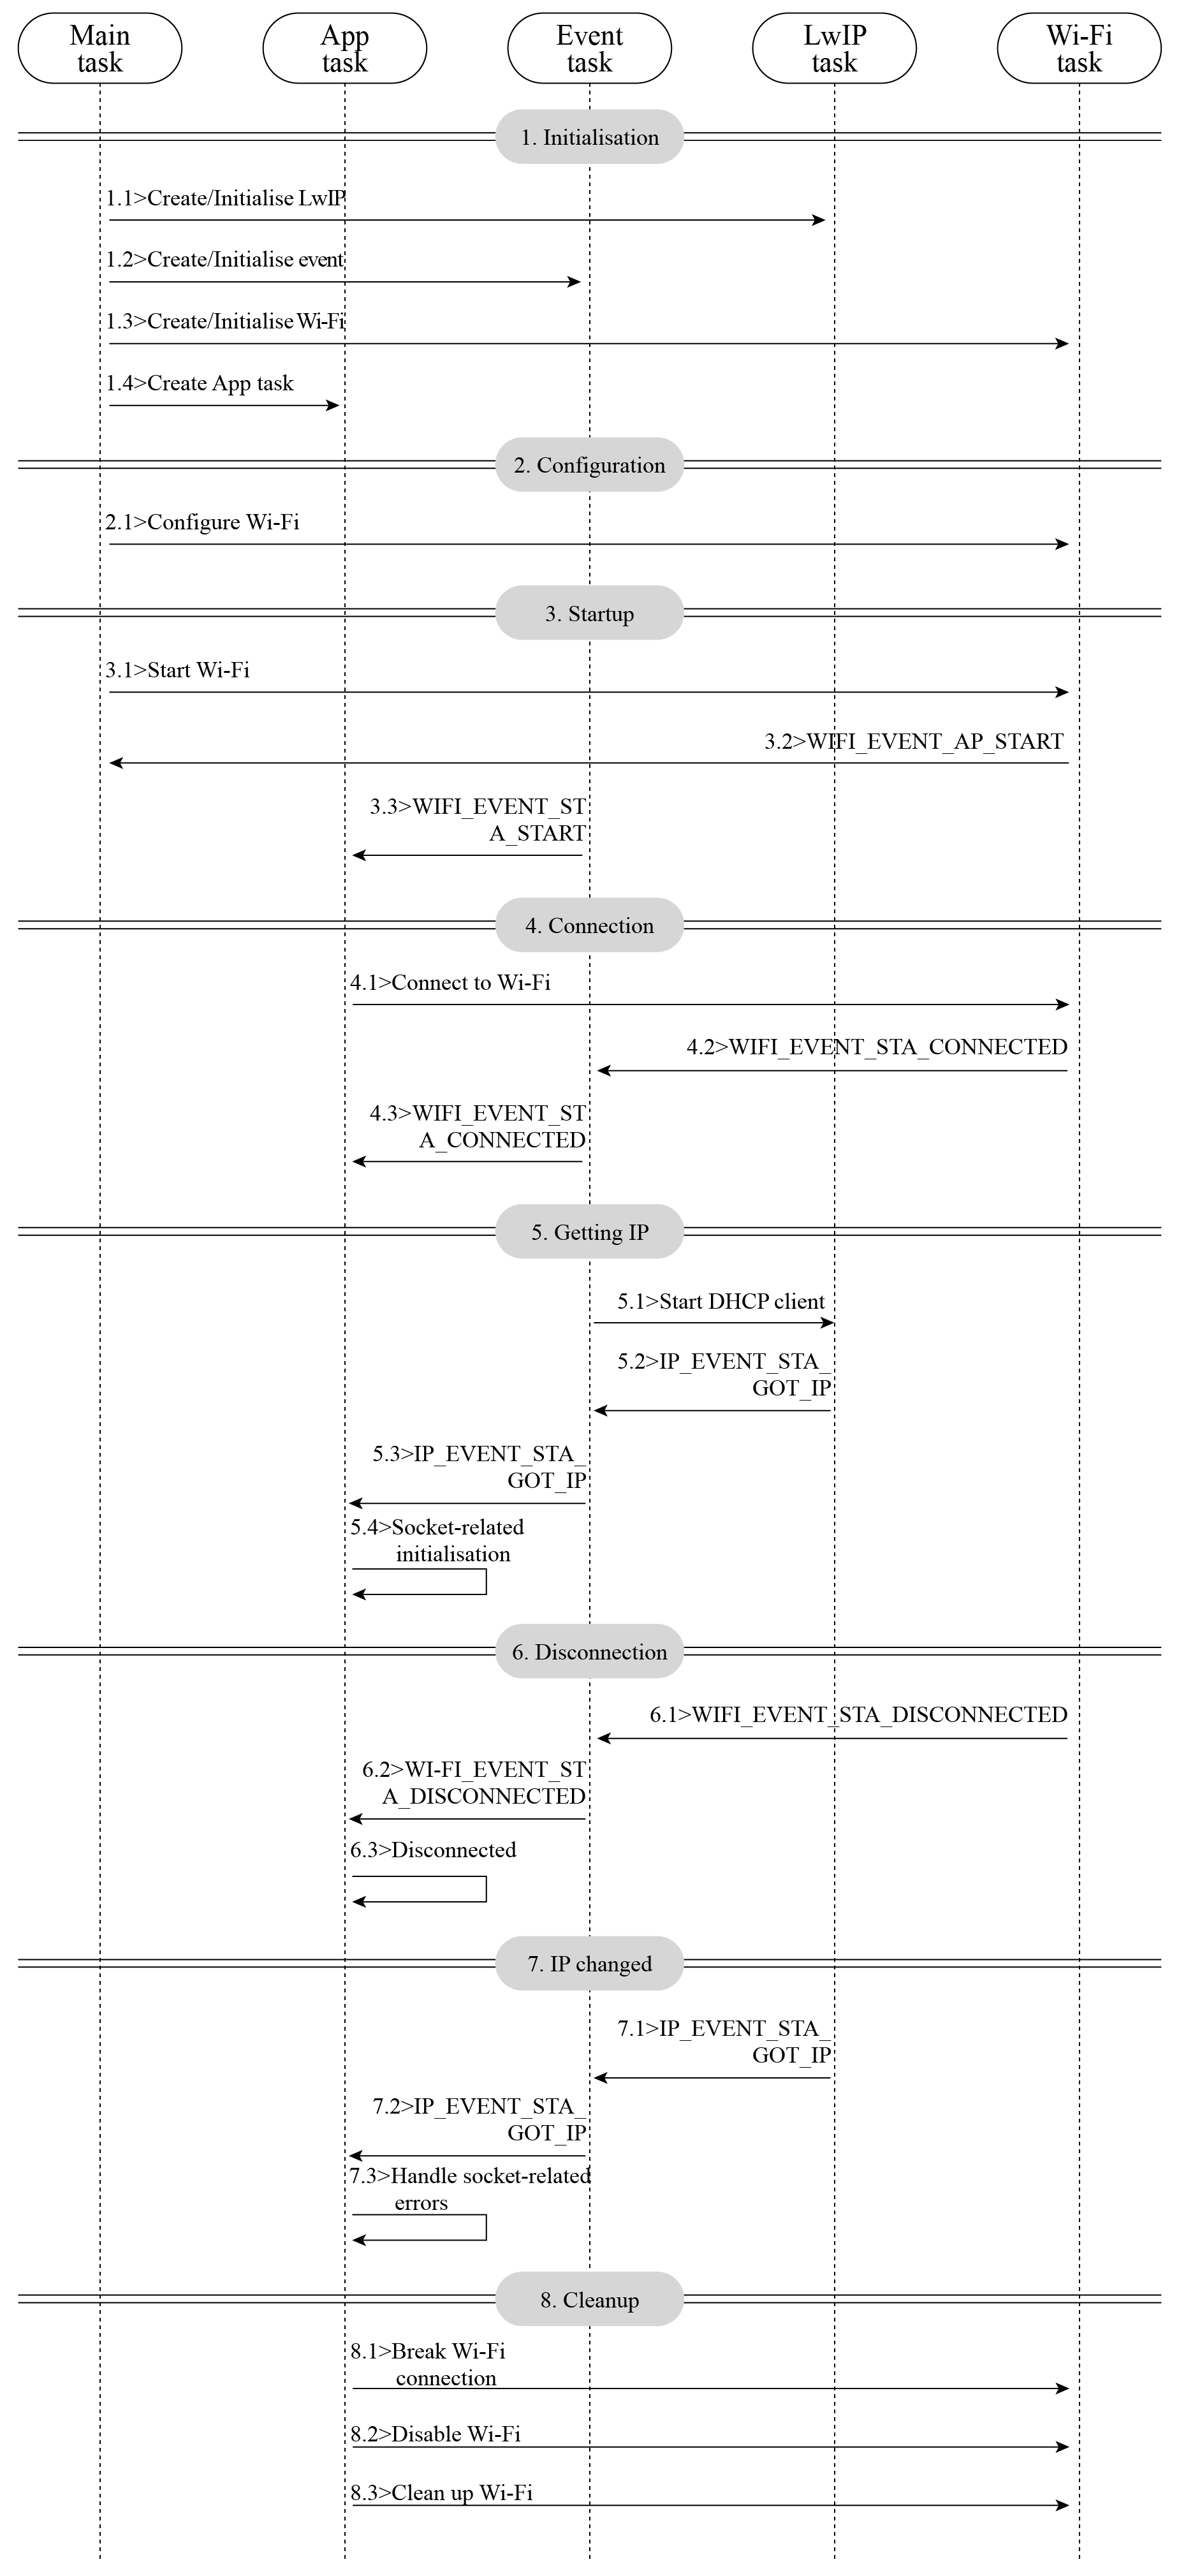
\includegraphics[width=0.67\textwidth]{D7Z/7-33}
    \caption{Using ESP-IDF components to connect devices to routers}
\end{figure}

\restoregeometry % restore original margins
        
b. \textbf{Initialise event}. As introduced before, Wi-Fi event handling is based on the \verb|esp_event| library, assisted by the \verb|esp_netif| component. The code to initialise the event is as follows:

\begin{codebloc}
\begin{tabular}{d}
\vspace{2pt}
\begin{verbatim}
1.  ESP_ERROR_CHECK(esp_event_loop_create_default());
2.  esp_netif_create_default_wifi_sta();
3.  esp_event_handler_instance_t instance_any_id;
4.  esp_event_handler_instance_t instance_got_ip;
5.  ESP_ERROR_CHECK(esp_event_handler_instance_register(WIFI_EVENT,
6.                                                      ESP_EVENT_ANY_ID,
7.                                                      &event_handler,
8.                                                      NULL,
9.                                                      &instance_any_id));
10. ESP_ERROR_CHECK(esp_event_handler_instance_register(IP_EVENT,
11.                                                     IP_EVENT_STA_GOT_IP,
12.                                                     &event_handler,
13.                                                     NULL,
\end{verbatim}
\verb|14.                                                     &instance_got_ip));|
\end{tabular}
\end{codebloc}

c. \textbf{Initialise Wi-Fi}. Create the Wi-Fi driver task, and initialise the Wi-Fi driver. The code to initialise Wi-Fi is as follows:

\begin{codebloc}
\begin{tabular}{d}
\verb|1.  wifi_init_config_t cfg = WIFI_INIT_CONFIG_DEFAULT();|

\verb|2.  ESP_ERROR_CHECK(esp_wifi_init(&cfg));|
\end{tabular}
\end{codebloc}

(2) \textbf{Configuration}. Once the Wi-Fi driver is initialised, you can start configuration. At this stage, the driver is in STA mode, so you may call \verb|esp_wifi_set_mode(WIFI_MODE_STA)| to put ESP32-C3 into STA mode. Refer to the code below:

\begin{codebloc}
\begin{tabular}{d}
\vspace{2pt}
\begin{verbatim}
1.  wifi_config_t wifi_config = {
2.      .sta = {
3.          .ssid = EXAMPLE_ESP_WIFI_SSID,
4.          .password = EXAMPLE_ESP_WIFI_PASS,
5.      },
6.  };
7.  ESP_ERROR_CHECK(esp_wifi_set_mode(WIFI_MODE_STA));
\end{verbatim}
\verb|8.  ESP_ERROR_CHECK(esp_wifi_set_config(WIFI_IF_STA, &wifi_config));|
\end{tabular}
\end{codebloc}

(3) \textbf{Startup}. Call \verb|esp_wifi_start()| to start the Wi-Fi driver.

\begin{codebloc}
\begin{tabular}{d}
\verb|1.  ESP_ERROR_CHECK(esp_wifi_start());|
\end{tabular}
\end{codebloc}

The Wi-Fi driver posts \verb|WIFI_EVENT_STA_START| to the event task; then, the event task will do some routine work and call the application event callback function.
    
The application event callback function relays \verb|WIFI_EVENT_STA_START| to the application task, and then we call \verb|esp_wifi_connect()|.

(4) \textbf{Connection}. Once \verb|esp_wifi_connect()| is called, the Wi-Fi driver will start the internal scan/connection process.

If the internal scan/connection is successful, \verb|WIFI_EVENT_STA_CONNECTED| will be generated. In the event task, the DHCP client will be started and trigger the DHCP process. Refer to the code below:

\begin{codebloc}
\begin{tabular}{d}
\vspace{2pt}
\begin{verbatim}
1.  static void event_handler(void* arg, esp_event_base_t event_base,
2.                            int32_t event_id, void* event_data)
3.  {
4.    if (event_base == WIFI_EVENT && event_id == WIFI_EVENT_STA_START) {
5.      esp_wifi_connect();
6.    } else if
7.      (event_base == WIFI_EVENT && event_id == WIFI_EVENT_STA_DISCONNECTED) {
8.      if (s_retry_num < EXAMPLE_ESP_MAXIMUM_RETRY) {
9.        esp_wifi_connect();
10.         s_retry_num++;
11.         ESP_LOGI(TAG, "retry to connect to the AP");
12.       } else {
13.         xEventGroupSetBits(s_wifi_event_group, WIFI_FAIL_BIT);
14.       }
15.       ESP_LOGI(TAG, "connect to the AP fail");
16.     } else if (event_base == IP_EVENT && event_id == IP_EVENT_STA_GOT_IP) {
17.       ip_event_got_ip_t* event = (ip_event_got_ip_t*) event_data;
18.       ESP_LOGI(TAG, "got ip:" IPSTR, IP2STR(&event->ip_info.ip));
19.       s_retry_num = 0;
20.       xEventGroupSetBits(s_wifi_event_group, WIFI_CONNECTED_BIT);
21.     }
\end{verbatim}
\verb|22. }|
\end{tabular}
\end{codebloc}

(5) \textbf{Getting IP}. Once the DHCP client is initialised, the “getting IP” phase will begin. If the IP address is successfully received from the DHCP server, \verb|IP_EVENT_STA_GOT_IP| will be triggered and commonly handled in event task.

In the application event callback, \verb|IP_EVENT_STA_GOT_IP| is relayed to the application task. For LwIP-based applications, this marks a special event which means that everything is ready for the application to perform subsequent tasks. But remember not to start the socket-related work before receiving the IP.

(6) \textbf{Disconnection}. Wi-Fi connection may fail because of active disconnection, wrong password, AP not found, etc. In this case, \verb|WIFI_EVENT_STA_DISCONNECTED| will arise and provide the reason for the failure, such as \verb|esp_wifi_disconnect()| being called to actively disconnect.

\begin{codebloc}
\begin{tabular}{d}
\verb|1.  ESP_ERROR_CHECK(esp_wifi_disconnect());|
\end{tabular}
\end{codebloc}

(7) \textbf{IP Changed}. If the IP address is changed, \verb|IP_EVENT_STA_GOT_IP| will be triggered with \verb|ip_change| set to \verb|true|.

(8) \textbf{Cleanup}, including breaking Wi-Fi connection, stopping and unloading the Wi-Fi driver, etc. The code is as follows:

\begin{codebloc}
\begin{tabular}{d}
\vspace{2pt}
\begin{verbatim}
1.  ESP_ERROR_CHECK(esp_event_handler_instance_unregister(IP_EVENT,
2.                                                        IP_EVENT_STA_GOT_IP,
3.                                                        instance_got_ip));
4.  ESP_ERROR_CHECK(esp_event_handler_instance_unregister(WIFI_EVENT,
5.                                                        ESP_EVENT_ANY_ID,
6.                                                        instance_any_id));
7.  ESP_ERROR_CHECK(esp_wifi_stop());
8.  ESP_ERROR_CHECK(esp_wifi_deinit());
9.  ESP_ERROR_CHECK(esp_wifi_clear_default_wifi_driver_and_handlers(
10.                 station_netif));
\end{verbatim}
\verb|11. esp_netif_destroy(station_netif);|
\end{tabular}
\end{codebloc}

\subsection{Exercise: Smart Wi-Fi Connection}
\textbf{1. SoftAP}

The \verb|wifi_provisioning| components provided by ESP32-C3 can transmit SSID and password of the AP through SoftAP or Bluetooth LE, and then use them to connect to the AP.

\textbf{(1) APIs}

The APIs for \verb|wifi_provisioning| are defined in \href{https://github.com/espressif/esp-idf/blob/master/components/wifi_provisioning/include/wifi_provisioning/manager.h}{\texttt{esp-idf/components/wifi\_provi\\ sioning/include/wifi\_provisioning/manager.h}}, as shown in Table 7.4.

\begin{table}[h!]
    \renewcommand{\arraystretch}{1}
    \caption{APIs for \texttt{wifi\_provisioning} components}
    \begin{tabular}{|>{\footnotesize}m{0.52\textwidth}|>{\footnotesize}m{0.46\textwidth}|}
        \hline
        \rowcolor{LightBlue}\multicolumn{1}{|c|}{\textbf{API}}&\multicolumn{1}{c|}{\textbf{Description}}\\
        \hline
        \verb|wifi_prov_mgr_init()|&Initialise \verb|provisioning| manager interface according to current configuration\\
        \hline
        \verb|wifi_prov_mgr_deinit()|&Release \verb|provisioning| manager interface\\
        \hline
        \verb|wifi_prov_mgr_is_provisioned()|&Check the \verb|provisioning| status of ESP32-C3\\
        \hline
        \verb|wifi_prov_mgr_start_provisioning()|&Start the \verb|provisioning| service\\
        \hline
        \verb|wifi_prov_mgr_stop_provisioning()|&Stop the \verb|provisioning| service\\
        \hline
        \verb|wifi_prov_mgr_wait()|&Wait for the \verb|provisioning| service to finish\\
        \hline
        \verb|wifi_prov_mgr_disable_auto_stop()|&Disable auto stopping of the \verb|provisioning| service upon completion\\
        \hline
        \verb|wifi_prov_mgr_endpoint_create()|&Create an \verb|endpoint| and allocate internal resources for it\\
        \hline
        \verb|wifi_prov_mgr_endpoint_register()|&Register a handler for the created \verb|endpoint|\\
        \hline
        \verb|wifi_prov_mgr_endpoint_unregister()|&Unregister the handler for the created \verb|endpoint|\\
        \hline
        \verb|wifi_prov_mgr_get_wifi_state()|&Get the state of the Wi-Fi STA during \verb|provisioning|\\
        \hline
        \verb|wifi_prov_mgr_get_wifi_disconnect_reason()|&Get the reason code for Wi-Fi STA disconnection during \verb|provisioning|\\
        \hline
    \end{tabular}
\end{table}

\textbf{(2) Program structure}

\textbullet\ Initialisation:

\begin{codebloc}
\begin{tabular}{d}
\vspace{2pt}
\begin{verbatim}
1.  wifi_prov_mgr_config_t config = {
2.      .scheme = wifi_prov_scheme_softap,
3.      .scheme_event_handler = WIFI_PROV_EVENT_HANDLER_NONE
4.  };
5.
\end{verbatim}
\verb|6.  ESP_ERR_CHECK(wifi_prov_mgr_init(config));|
\end{tabular}
\end{codebloc}

\textbullet\ Checking the \verb|provisioning| status:

\begin{codebloc}
\begin{tabular}{d}
\verb|1.  bool provisioned = false;|

\verb|2.  ESP_ERROR_CHECK(wifi_prov_mgr_is_provisioned(&provisioned));|
\end{tabular}
\end{codebloc}

\textbullet\ Starting \verb|provisioning| service:

\begin{codebloc}
\begin{tabular}{d}
\vspace{2pt}
\begin{verbatim}
1.  const char *service_name = "my_device";
2.  const char *service_key  = "password";
3.
4.  wifi_prov_security_t security = WIFI_PROV_SECURITY_1;
5.  const char *pop = "abcd1234";
6.
7.  ESP_ERR_CHECK(wifi_prov_mgr_start_provisioning(security, pop, service_name,
\end{verbatim}
\verb|8.                service_key));|
\end{tabular}
\end{codebloc}

\textbullet\ Releasing resources for \verb|provisioning|.

Once the \verb|provisioning| service is complete, the main application will release the resources for \verb|provisioning| and start executing its own logic. There are two ways to do this. The simpler way is to call \verb|wifi_prov_mgr_wait()|. See the code below:

\begin{codebloc}
\begin{tabular}{d}
\vspace{2pt}
\begin{verbatim}
1.  //Wait for the provisioning service to finish
2.  wifi_prov_mgr_wait();
3.
4.  //Release the resources for provisioning
\end{verbatim}
\verb|5.  wifi_prov_mgr_deinit();|
\end{tabular}
\end{codebloc}

The other way is to use the callback function of the event. See the code below:

\begin{codebloc}
\begin{tabular}{d}
\vspace{2pt}
\begin{verbatim}
1.  static void event_handler(void* arg, esp_event_base_t event_base,
2.                            int event_id, void* event_data)
3.  {
4.      if (event_base == WIFI_PROV_EVENT && event_id == WIFI_PROV_END) {
5.          //Release the resources for provisioning upon completion
6.          wifi_prov_mgr_deinit();
7.      }
\end{verbatim}
\verb|8.  }|
\end{tabular}
\end{codebloc}

\textbf{(3) Functional verification}

To get started, install ESP SoftAP Provisioning on your phone. Next, turn on the Wi-Fi and power on the device. Ensure that the output log by the serial port (see Figure 7.34) contains information beginning with \verb|PROV_|. 

\note{You may download the APP at \url{https://www.espressif.com/en/support/download/apps}.}

\begin{figure}[!h]
    \centering
    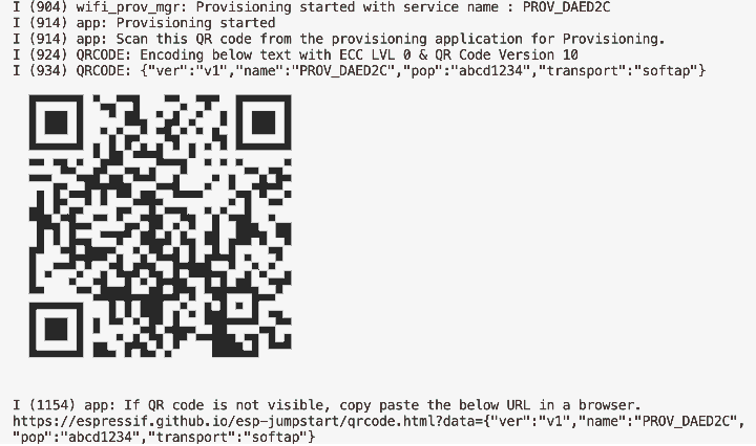
\includegraphics[width=0.8\textwidth]{D7Z/7-34}
    \caption{Output log by the serial port}
\end{figure}

\textbf{a. Startup}

Open the application on your phone and tap “Start Provisioning”. Then you will find the device PROV\_DAED2CXXXXX on the screen (refer to Figure 7.35).

\begin{figure}[!h]
  \Centering
  \begin{minipage}[b]{0.4\textwidth}
    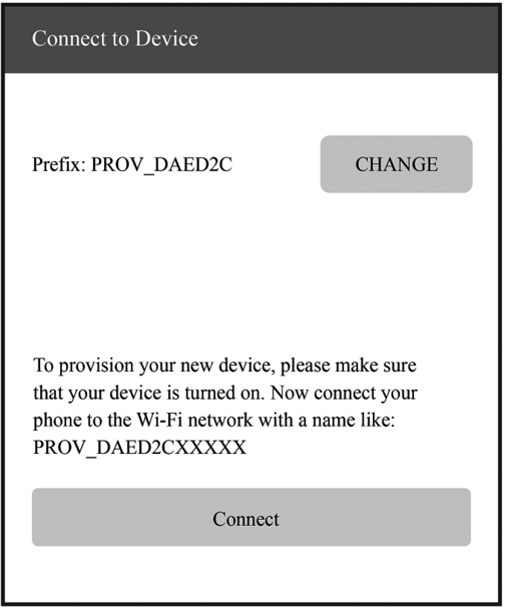
\includegraphics[width=0.95\textwidth]{D7Z/7-35}
    \caption{Startup}
  \end{minipage}\hspace{1em}
  \begin{minipage}[b]{0.4\textwidth}
    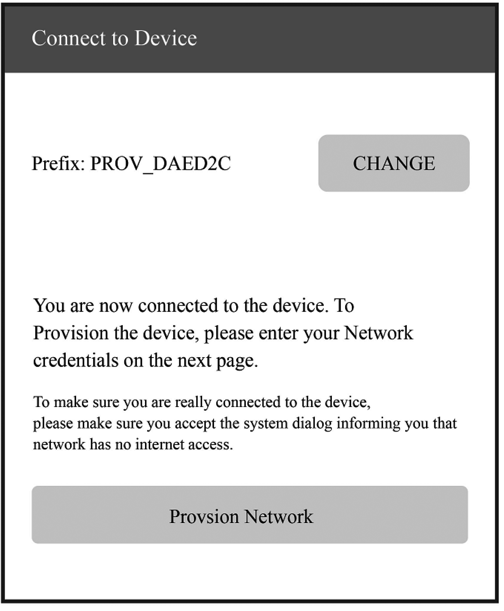
\includegraphics[width=0.95\textwidth]{D7Z/7-36}
    \caption{SoftAP connection}
  \end{minipage}
\end{figure}

\textbf{b. Connection}

Tap “Connect” to navigate to the Wi-Fi setting interface. Select to connect the device PROV\_DAED2CXXXXX. If connected, you will see the screen as Figure 7.36.

The output log is as follows:

\begin{codebloc}
\fontsize{8pt}{8pt}\selectfont
\begin{tabular}{d}
\vspace{2pt}
\begin{verbatim}
I (102906) wifi:station: 88:40:3b:40:c1:13 join, AID=1, bgn, 40U
I (103056) esp_netif_lwip: DHCP server assigned IP to a station, IP is: 192.168.4.2
I (124286) wifi:station: 88:40:3b:40:c1:13 leave, AID = 1, bss_flags is 134259, bss:0x3fca7844
I (124286) wifi:new: <1,0>, old: <1,1>, ap: <1,1>, sta: <0,0>, prof:1
I (149036) wifi:new: <1,1>, old: <1,0>, ap: <1,1>, sta: <0,0>, prof:1
I (149036) wifi:station: 88:40:3b:40:c1:13 join, AID=1, bgn, 40U
\end{verbatim}
\verb|I (149246) esp_netif_lwip: DHCP server assigned IP to a station, IP is: 192.168.4.2|
\end{tabular}
\end{codebloc}

\textbf{c. Provisioning}

Tap “Provision Network” to enter the provisioning screen shown in Figure 7.37.

\textbf{d. Completion}

Tap “Provision” to enter the completion screen shown in Figure 7.38.

\begin{figure}[!h]
  \Centering
  \begin{minipage}[b]{0.4\textwidth}
    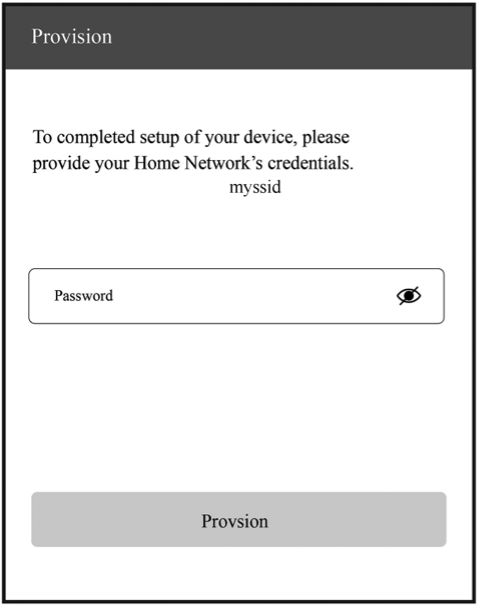
\includegraphics[width=0.95\textwidth]{D7Z/7-37}
    \caption{Provisioning}
  \end{minipage}\hspace{1em}
  \begin{minipage}[b]{0.4\textwidth}
    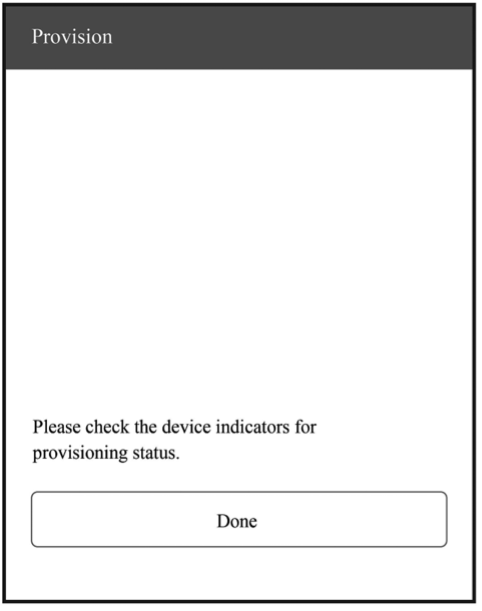
\includegraphics[width=0.95\textwidth]{D7Z/7-38}
    \caption{Completion}
  \end{minipage}
\end{figure}

The output log is as follows:

\begin{codebloc}
\fontsize{8pt}{8pt}\selectfont
\begin{tabular}{d}
\vspace{2pt}
\begin{verbatim}
I (139471) app: Received Wi-Fi credentials
          SSID     : myssid
          Password : mypassword
          .
          .
          .
I (144091) app: Connected with IP Address:192.168.50.31
I (144091) esp_netif_handlers: sta ip: 192.168.50.31, mask: 255.255.255.0, gw: 192.168.50.1
I (144091) wifi_prov_mgr: STA Got IP
I (144101) app: provisioningsuccessful
I (144101) app: Hello World!
I (145101) app: Hello World!
          .
\end{verbatim}
\verb|          .|
\end{tabular}
\end{codebloc}

\begin{codebloc}
\fontsize{8pt}{8pt}\selectfont
\begin{tabular}{d}
\vspace{2pt}
\begin{verbatim}
          .
I (146091) wifi_prov_mgr: Provisioning stopped
I (146101) app: Hello World!
I (147101) app: Hello World!
\end{verbatim}
\verb|I (148101) app: Hello World!|
\end{tabular}
\end{codebloc}

\textbf{2. SmartConfig}

The SmartConfig component provided by ESP32-C3 can transmit the SSID and password of the AP through promiscuous mode, and then use them to connect to the AP.

\textbf{(1) APIs}

The APIs for SmartConfig are defined in \href{https://github.com/espressif/esp-idf/blob/master/components/esp_wifi/include/esp_smartconfig.h}{\texttt{esp-idf/components/esp\_wifi/include/\\ esp\_smartconfig.h}}, as shown in Table 7.5.

\begin{table}[h!]
    \renewcommand{\arraystretch}{1.5}
    \caption{APIs for SmartConfig}
    \begin{tabular}{|>{\small}m{0.48\textwidth}|>{\small}m{0.5\textwidth}|}
        \hline
        \rowcolor{LightBlue}\multicolumn{1}{|c|}{\textbf{API}}&\multicolumn{1}{c|}{\textbf{Description}}\\
        \hline
        \verb|esp_smartconfig_get_version()|&Get the version of the current SmartConfig\\
        \hline
        \verb|esp_smartconfig_start()|&Start SmartConfig\\
        \hline
        \verb|esp_smartconfig_stop()|&Stop SmartConfig\\
        \hline
        \verb|esp_esptouch_set_timeout()|&Set the timeout of SmartConfig process\\
        \hline
        \verb|esp_smartconfig_set_type()|&Set the protocol type of SmartConfig\\
        \hline
        \verb|esp_smartconfig_fast_mode()|&Set the mode of SmartConfig\\
        \hline
        \verb|esp_smartconfig_get_rvd_data()|&Get the reserved data of ESPTouch v2\\
        \hline
    \end{tabular}
\end{table}

\textbf{(2) Program structure}

\textbullet\ Wi-Fi event handling

This module takes care of Wi-Fi connection, disconnection, reconnection, scanning, etc., as detailed in the sections before. Additionally, when the \verb|WIFI_EVENT_STA_START| event occurs, it will also create a SmartConfig task.

\textbullet\ NETIF event handling

This module helps acquire the IP address. Details are provided in the sections before. When the \verb|IP_EVENT_STA_GOT_IP| event occurs, the connection flag will be set.

\textbullet\ SmartConfig event handling

The received request determines how the event is handled and processed. SmartConfig events are shown in Table 7.6.

\begin{table}[h!]
    \renewcommand{\arraystretch}{1.2}
    \caption{SmartConfig events}
    \begin{tabular}{|>{\small}m{0.32\textwidth}|>{\small}m{0.66\textwidth}|}
        \hline
        \rowcolor{LightBlue}\multicolumn{1}{|c|}{\textbf{Event}}&\multicolumn{1}{c|}{\textbf{Description}}\\
        \hline
        \verb|SC_EVENT_SCAN_DONE|&Scan to obtain the information about nearby APs\\
        \hline
        \verb|SC_EVENT_FOUND_CHANNEL|&Get the channel of the target AP\\
        \hline
        \verb|SC_EVENT_GOT_SSID_PSWD|&Enter STA mode to get the SSID and password of the target AP\\
        \hline
        \verb|SC_EVENT_SEND_ACK_DONE|&Set the SmartConfig completion flag\\
        \hline
    \end{tabular}
\end{table}

\textbullet\ SmartConfig tasks

The code for SmartConfig tasks is as follows.

\begin{codebloc}
\begin{tabular}{d}
\vspace{2pt}
\begin{verbatim}
1.  static void smartconfig_example_task (void *param)
2.  {
3.      EventBits_t uxBits;
4.      ESP_ERROR_CHECK(esp_smartconfig_set_type(SC_TYPE_ESPTOUCH));
5.      smartconfig_start_config_t cfg = SMARTCONFIG_START_CONFIG_DEFAULT();
6.      ESP_ERROR_CHECK(esp_smartconfig_start(&cfg));
7.      while (1) {
8.          uxBits = xEventGroupWaitBits (s_wifi_event_group,
9.                                        CONNECTED_BIT | ESPTOUCH_DONE_BIT,
10.                                       true,
11.                                       false,
12.                                       portMAX_DELAY);
13.         if (uxBits & CONNECTED_BIT) {
14.             ESP_LOGI (TAG, "WiFi Connected to ap");
15.         }
16.         if (uxBits & ESPTOUCH_DONE_BIT) {
17.             ESP_LOGI (TAG, "smartconfig over");
18.             esp_smartconfig_stop();
19.             vTaskDelete (NULL);
20.         }
21.     }
\end{verbatim}
\verb|22. }|
\end{tabular}
\end{codebloc}

As demonstrated in the code above, a SmartConfig task primarily performs three functions. First, it sets the SmartConfig type, such as ESP-TOUCH and ESP-TOUCH V2. Second, after the configuration, it enables SmartConfig by calling \verb|esp_smartconfig_start()|. Finally, it checks the event group in a loop. Upon receiving the \verb|SC_EVENT_SEND_ACK_DONE| event, it stops SmartConfig by calling \verb|esp_smartconfig_stop()|.

\textbullet\ Main program

It creates an event group to set the flag when a relevant event is triggered, and then initialises Wi-Fi.

\textbf{(3) Functional verification}

To get started, install Espressif Esptouch on your phone. Then turn on the Wi-Fi and power on the device. You will see the output log by the serial port as follows:

\begin{codebloc}
\begin{tabular}{d}
\vspace{2pt}
\begin{verbatim}
I (1084) wifi:mode : sta (30:ae:a4:80:65:7c)
I (1084) wifi:enable tsf
I (1134) smartconfig: SC version: V3.0.1
I (5234) wifi:ic_enable_sniffer
I (5234) smartconfig: Start to find channel...
\end{verbatim}
\verb|I (5234) smartconfig_example: Scan done|
\end{tabular}
\end{codebloc}

\note{You may download the APP at \url{https://www.espressif.com/en/support/download/apps}.}

Connect your phone to Wi-Fi, and enter the password to start configuration. The SmartConfig interface is shown in Figure 7.39.

\begin{figure}[!h]
    \centering
    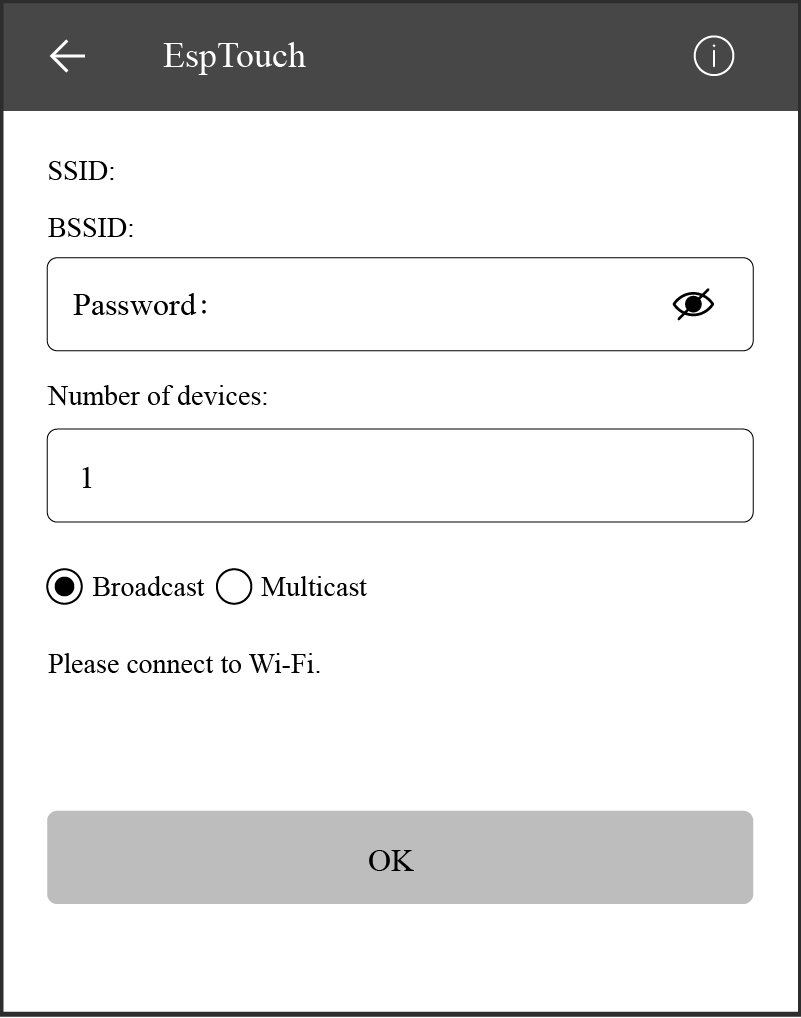
\includegraphics[width=0.4\textwidth]{D7Z/7-39}
    \caption{SmartConfig configuration}
\end{figure}

The output log is as follows:

\begin{codebloc}
\begin{tabular}{d}
\vspace{2pt}
\begin{verbatim}
I (234592) smartconfig: TYPE: ESPTOUCH
I (234592) smartconfig: T|PHONE MAC:68:3e:34:88:59:bf
I (234592) smartconfig: T|AP MAC:a4:56:02:47:30:07
I (234592) sc: SC_STATUS_GETTING_SSID_PSWD
I (239922) smartconfig: T|pswd: 123456789
I (239922) smartconfig: T|ssid: IOT_DEMO_TEST
I (239922) smartconfig: T|bssid: a4:56:02:47:30:07
\end{verbatim}
\verb|I (239922) wifi: ic_disable_sniffer|
\end{tabular}
\end{codebloc}

\begin{codebloc}
\begin{tabular}{d}
\vspace{2pt}
\begin{verbatim}
I (239922) sc: SC_STATUS_LINK
I (239932) sc: SSID:IOT_DEMO_TEST
I (239932) sc: PASSWORD:123456789
I (240062) wifi: n:1 0, o:1 0, ap:255 255, sta:1 0, prof:1
I (241042) wifi: state: init -> auth (b0)
I (241042) wifi: state: auth -> assoc (0)
I (241052) wifi: state: assoc -> run (10)
I (241102) wifi: connected with IOT_DEMO_TEST, channel 1
I (244892) event: ip: 192.168.0.152, mask: 255.255.255.0, gw: 192.168.0.1
I (244892) sc: WiFi Connected to ap
I (247952) sc: SC_STATUS_LINK_OVER
I (247952) sc: Phone ip: 192.168.0.31
\end{verbatim}
\verb|I (247952) sc: smartconfig over|
\end{tabular}
\end{codebloc}

\textbf{3. Bluetooth}

The BluFi components of ESP32-C3 help transmit the SSID and password through Bluetooth LE, which can be used to connect to the AP.

\textbf{(1) APIs}

The APIs for BluFi components are defined in \href{https://github.com/espressif/esp-idf/blob/master/components/bt/common/api/include/api/esp_blufi_api.h}{\texttt{esp\_blufi\_api.h}}, as shown in Table 7.7.

\begin{table}[h!]
    \renewcommand{\arraystretch}{1.1}
    \caption{APIs for BluFi components}
    \begin{tabular}{|>{\small}m{0.5\textwidth}|>{\small}m{0.48\textwidth}|}
        \hline
        \rowcolor{LightBlue}\multicolumn{1}{|c|}{\textbf{API}}&\multicolumn{1}{c|}{\textbf{Description}}\\
        \hline
        \verb|esp_blufi_register_callbacks()|&Register BluFi callback events\\
        \hline
        \verb|esp_blufi_profile_init()|&Initialise BluFi profile\\
        \hline
        \verb|esp_blufi_profile_deinit()|&Deinitialise BluFi profile\\
        \hline
        \verb|esp_blufi_send_wifi_conn_report()|&Send Wi-Fi connection reports\\
        \hline
        \verb|esp_blufi_send_wifi_list()|&Send the Wi-Fi list\\
        \hline
        \verb|esp_blufi_get_version()|&Get the version of the current BluFi profile\\
        \hline
        \verb|esp_blufi_close()|&Disconnect the device\\
        \hline
        \verb|esp_blufi_send_error_info()|&Send BluFi error messages\\
        \hline
        \verb|esp_blufi_send_custom_data()|&Send custom data\\
        \hline
    \end{tabular}
\end{table}

\textbf{(2) Program structure}

\begin{itemize}[leftmargin=1.5em]
    \item \textbf{Wi-Fi event handling}: taking care of Wi-Fi connection, disconnection, reconnection, scanning, etc., as detailed in the sections before.
    \item \textbf{NETIF event handling}: acquiring IP address. Details are provided in the sections before.
    \item \textbf{BluFi event handling}: determined by the received request. BluFi events are shown in Table 7.8.

{\renewcommand{\arraystretch}{1.2}
\begin{longtable}{|>{\scriptsize}m{0.43\textwidth}|>{\footnotesize}m{0.55\textwidth}|}
    \caption{BluFi events \label{7.8}} \\
        
    \hline
    \rowcolor{LightBlue}\multicolumn{1}{|c|}{\textbf{Event}}&\multicolumn{1}{c|}{\textbf{Description}}\\
    \hline
    \endfirsthead

    \multicolumn{2}{r}{Continuation of Table \ref{7.8}}\\
    \hline
    \rowcolor{LightBlue}\multicolumn{1}{|c|}{\textbf{Event}}&\multicolumn{1}{c|}{\textbf{Description}}\\
    \hline
    \endhead
        
    \verb|ESP_BLUFI_EVENT_INIT_FINISH|&Initialise BluFi features, name the device, and send specified broadcast data\\
    \hline
    \verb|ESP_BLUFI_EVENT_DEINIT_FINISH|&Handle deinit configuration events\\
    \hline
    \verb|ESP_BLUFI_EVENT_BLE_CONNECT|&Connect to Bluetooth LE and put the device into safe mode\\
    \hline
    \verb|ESP_BLUFI_EVENT_BLE_DISCONNECT|&Set Bluetooth LE to disconnect and reconnect\\
    \hline
    \verb|ESP_BLUFI_EVENT_SET_WIFI_OPMODE|&Put ESP32-C3 into operating mode\\
    \hline
    \verb|ESP_BLUFI_EVENT_REQ_CONNECT_TO_AP|&Disconnect from the original Wi-Fi and connect to the specified Wi-Fi\\
    \hline
    \verb|ESP_BLUFI_EVENT_REQ_DISCONNECT_FROM_AP|&Disconnect from the AP currently connected to ESP32-C3\\
    \hline
    \verb|ESP_BLUFI_EVENT_REPORT_ERROR|&Send error messages\\
    \hline
    \verb|ESP_BLUFI_EVENT_GET_WIFI_STATUS|&Get Wi-Fi status, including the current Wi-Fi mode and whether it is connected\\
    \hline
    \verb|ESP_BLUFI_EVENT_RECV_SLAVE_DISCONNECT_BLE|&Notify BluFi that the GATT connection is closed\\
    \hline
    \verb|ESP_BLUFI_EVENT_RECV_STA_BSSID|&Enter STA mode and get the BSSID of the target AP\\
    \hline
    \verb|ESP_BLUFI_EVENT_RECV_STA_SSID|&Enter STA mode and get the SSID of the target AP\\
    \hline
    \verb|ESP_BLUFI_EVENT_RECV_STA_PASSWD|&Enter STA mode and get the password of the target AP\\
    \hline
    \verb|ESP_BLUFI_EVENT_RECV_SOFTAP_SSID|&Enter SoftAP mode and get the custom AP SSID\\
    \hline
    \verb|ESP_BLUFI_EVENT_RECV_SOFTAP_PASSWD|&Enter SoftAP mode and get the custom AP password\\
    \hline
    \verb|ESP_BLUFI_EVENT_RECV_SOFTAP_MAX_CONN_NUM|&Set the maximum number of connected devices in SoftAP mode\\
    \hline
    \verb|ESP_BLUFI_EVENT_RECV_SOFTAP_AUTH_MODE|&Enter authentication mode in SoftAP mode\\
    \hline
    \verb|ESP_BLUFI_EVENT_RECV_SOFTAP_CHANNEL|&Set the channel in SoftAP mode\\
    \hline
    \verb|ESP_BLUFI_EVENT_GET_WIFI_LIST|&Obtain the SSID list, channel, and STA MAC address scanned over the air\\
    \hline
    \verb|ESP_BLUFI_EVENT_RECV_CUSTOM_DATA|&Print the received data and trim it to fit the application\\
    \hline
\end{longtable}
}

    \item \textbf{Main program}: initialising Wi-Fi, initialising and enabling Bluetooth controller, initialising and enabling Bluetooth protocol, obtaining Bluetooth address and BluFi version, processing Bluetooth GAP events, and creating BluFi events.
\end{itemize}

\textbf{(3) Functional verification}

To get started, install EspBlufi on your phone. Turn on the Wi-Fi and power on the device. You will see the output log by the serial port as follows:

\begin{codebloc}
\fontsize{10pt}{10pt}\selectfont
\begin{tabular}{d}
\vspace{2pt}
\begin{verbatim}
I (516) phy_init: phy_version 500,985899c,Apr 19 2021,16:05:08
I (696) wifi:set rx active PTI: 0, rx ack PTI: 12, and default PTI: 1
I (908) wifi:mode : sta (30:ae:a4:80:41:55)
I (908) wifi:enable tsf
W (706) BTDM_INIT: esp_bt_controller_mem_release not implemented, return OK
I (706) BTDM_INIT: BT controller compile version [9c99115]
I (716) coexist: coexist rom version 9387209
I (726) BTDM_INIT: Bluetooth MAC: 30:ae:a4:80:41:56
I (746) BLUFI_EXAMPLE: BD ADDR: 30:ae:a4:80:41:56
I (1198) BLUFI_EXAMPLE: BLUFI VERSION 0102
\end{verbatim}
\verb|I (1198) BLUFI_EXAMPLE: BLUFI init finish|
\end{tabular}
\end{codebloc}

\note{You may download the APP at \url{https://www.espressif.com/en/support/download/apps}.}

\textbf{a. Startup}

Open the application on your phone and pull down to refresh. You will see the information about nearby Bluetooth devices on the screen as shown in Figure 7.40.

\textbf{b. Connection}

Select the ESP32-C3 module BLUFI\_DEVICE to get details about the device. Tap “Connect” to connect with Bluetooth. If connected, you will see the interface as Figure 7.41.

\begin{figure}[!h]
  \Centering
  \begin{minipage}[b]{0.4\textwidth}
    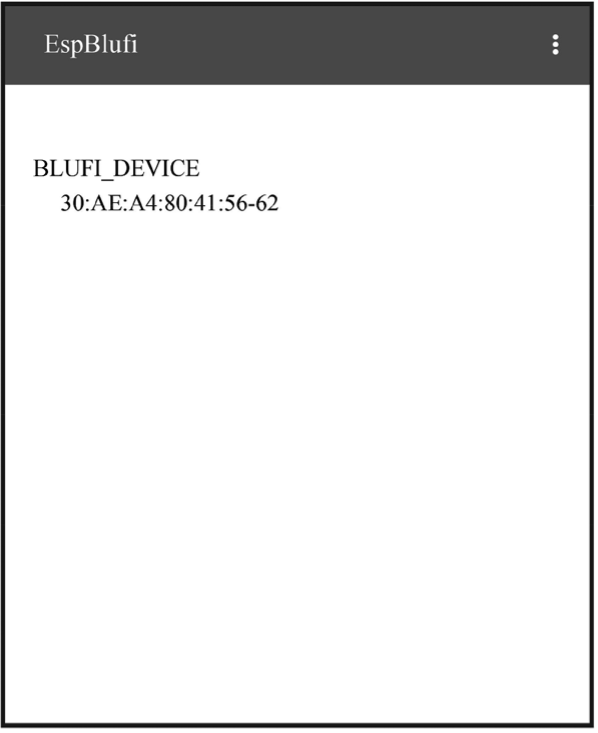
\includegraphics[height=1.3\textwidth]{D7Z/7-40}
    \caption{EspBlufi startup}
  \end{minipage}\hspace{2em}
  \begin{minipage}[b]{0.4\textwidth}
    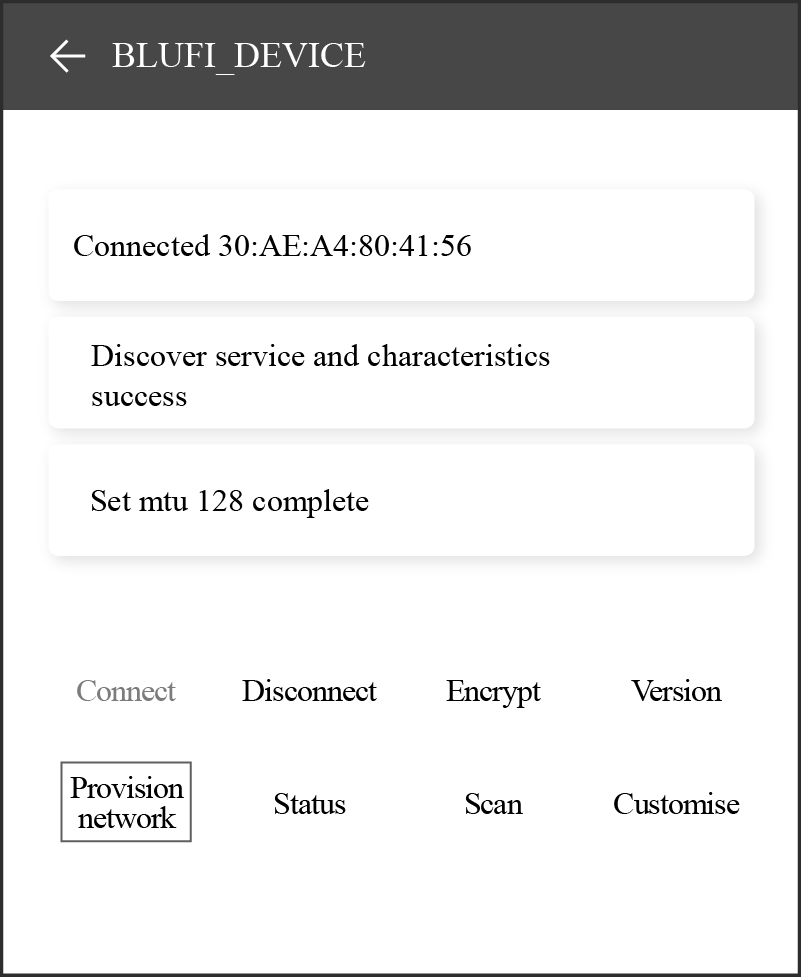
\includegraphics[height=1.29\textwidth,frame]{D7Z/7-41}
    \caption{Bluetooth connected}
  \end{minipage}
\end{figure}

The output log is as follows:

\begin{codebloc}
\begin{tabular}{d}
\verb|I (32736) BLUFI_EXAMPLE: BLUFI ble connect|
\end{tabular}
\end{codebloc}

\textbf{c. Provisioning}

Tap “Provision network” in Figure 7.41 to enter the provisioning interface shown in Figure 7.42.

\textbf{d. STA connection}

Tap “OK” in Figure 7.42 to configure the network. If the configuration succeeds, you will see the STA connected interface shown in Figure 7.43. Details about STA connection in Wi-Fi mode will be displayed at the bottom of the screen, including the BSSID and SSID of the AP and the connection status.

\begin{figure}[!h]
  \Centering
  \begin{minipage}[b]{0.4\textwidth}
    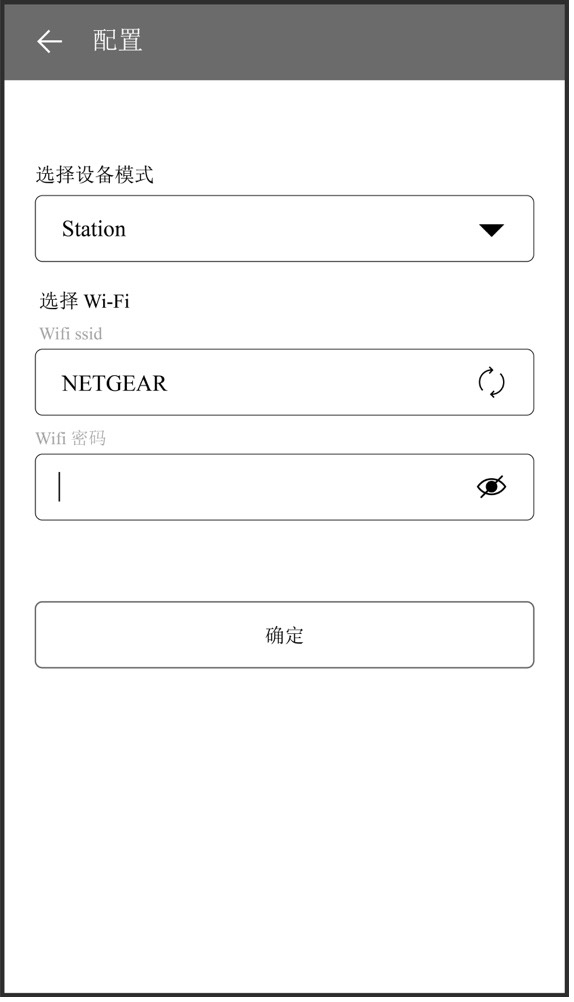
\includegraphics[width=\textwidth]{D7Z/7-42}
    \caption{Provisioning}
  \end{minipage}\hspace{2em}
  \begin{minipage}[b]{0.4\textwidth}
    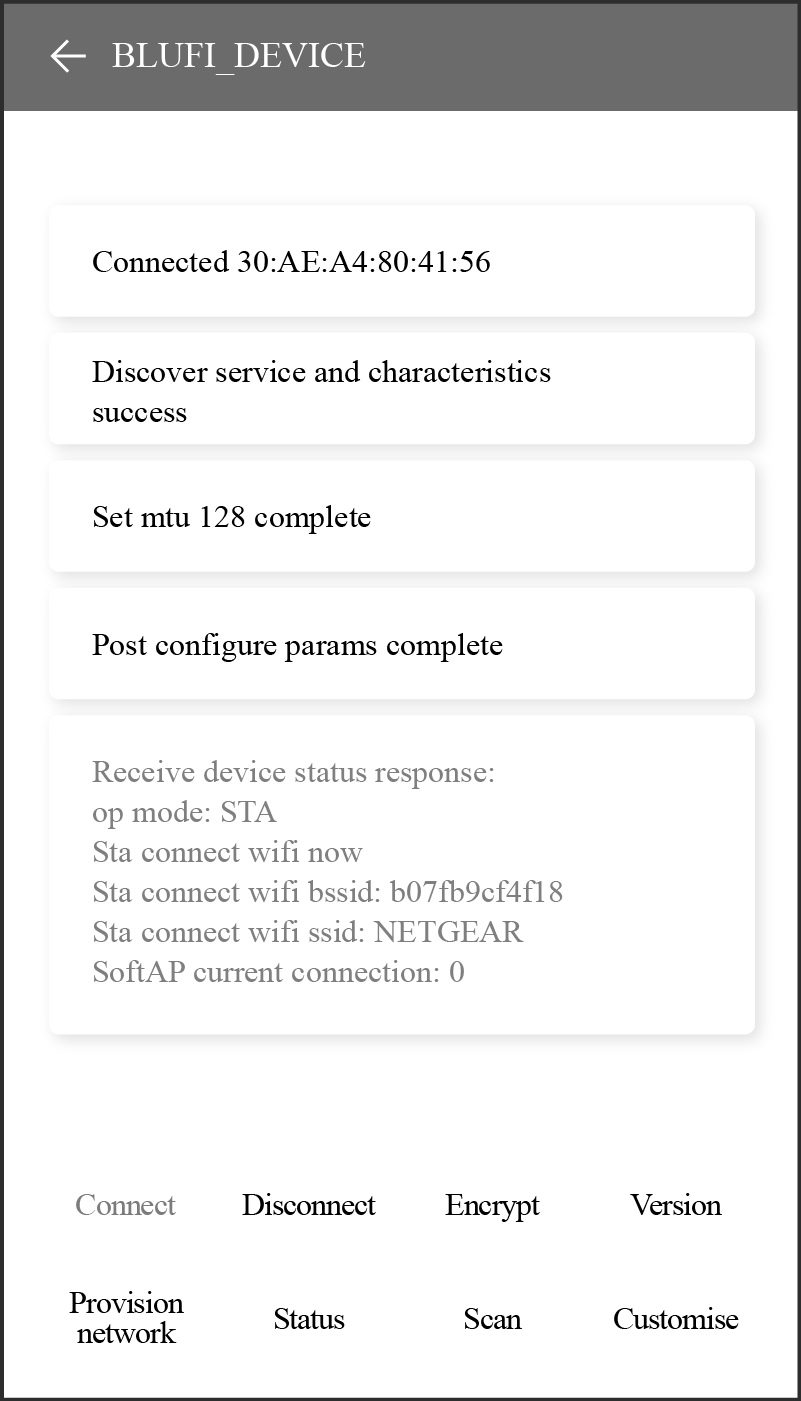
\includegraphics[width=\textwidth]{D7Z/7-43}
    \caption{STA connected}
  \end{minipage}
\end{figure}

The output log is as follows:

\begin{codebloc}
\fontsize{9.9pt}{9.9pt}\selectfont
\begin{tabular}{d}
\vspace{2pt}
\begin{verbatim}
I (63756) BLUFI_EXAMPLE: BLUFI Set WIFI opmode 1
I (63826) BLUFI_EXAMPLE: Recv STA SSID NETGEAR
I (63866) BLUFI_EXAMPLE: Recv STA PASSWORD 12345678
I (63936) BLUFI_EXAMPLE: BLUFI requset wifi connect to AP
I (65746) wifi:new: <8,2>, old: <1,0>, ap: <255,255>, sta: <8,2>, prof:1
I (66326) wifi:state: init -> auth (b0) 
I (67326) wifi:state: auth -> init (200) 
I (67326) wifi:new: <8,0>, old: <8,2>, ap: <255,255>, sta: <8,2>, prof:1 
I (69516) wifi:new: <10,0>, old: <8,0>, ap: <255,255>, sta: <10,0>, prof:1 
\end{verbatim} 
\verb|I (69516) wifi:state: init -> auth (b0) |
\end{tabular}
\end{codebloc}

\begin{codebloc}
\fontsize{9.9pt}{9.9pt}\selectfont
\begin{tabular}{d}
\vspace{2pt}
\begin{verbatim}
I (69566) wifi:state: auth -> assoc (0)
I (69626) wifi:state: assoc -> run (10) 
I (69816) wifi:connected with NETGEAR, aid = 1, channel 10, BW20, bssid = 5c:02:
14:03:a5:7d
I (69816) wifi:security: WPA2-PSK, phy: bgn, rssi: -48
I (69826) wifi:pm start, type: 1
I (69826) wifi:set rx beacon pti, rx_bcn_pti: 14, bcn_timeout: 14, mt_pti: 25000,
mt_time: 10000
I (69926) wifi:BcnInt:102400, DTIM:1 W (70566) wifi:idx:0 (ifx:0, 5c:02:14:03:a5:
7d), tid:0, ssn:2, winSize:64
I (71406) esp_netif_handlers: sta ip: 192.168.31.145, mask: 255.255.255.0, gw:
\end{verbatim} 
\verb|192.168.31.1|
\end{tabular}
\end{codebloc}

\section{Practice: Wi-Fi Configuration in Smart Light Project}
In this section, we will start by programming for Wi-Fi connection based on the LED dimming driver project, and then give an example of smart Wi-Fi configuration with the Smart Light project.

\subsection{Wi-Fi Connection in Smart Light Project}
After learning the basics of Wi-Fi connection, we may put it into practice based on ESP32-C3, and encapsulate the Wi-Fi features according to application requirements, so as to provide APIs for Wi-Fi initialisation and Wi-Fi connection initialisation.

\textbf{1. Driver initialisation}

This API specifies parameters for ESP32-C3, such as GPIO pins, fading time, breathing cycle, PWM frequency, clock source of the PWM controller, and PWM duty cycle resolution. For details, please refer to Chapter 5.

\begin{codebloc}
\begin{tabular}{d}
\verb|1.  app_driver_init();|
\end{tabular}
\end{codebloc}

\textbf{2. NVS initialisation}

Before initialising Wi-Fi, it is necessary to initialise the NVS library as the Wi-Fi component needs to acquire and store certain parameters. The API is as follows:

\begin{codebloc}
\begin{tabular}{d}
\verb|1.  nvs_flash_init();|
\end{tabular}
\end{codebloc}

\textbf{3. Wi-Fi initialisation}

This API handles LwIP and Wi-Fi events, and initialises Wi-Fi drivers.

\begin{codebloc}
\begin{tabular}{d}
\verb|1.  wifi_initialize();|
\end{tabular}
\end{codebloc}

\textbf{4. Wi-Fi connection initialisation}

This API implements Wi-Fi configuration, starts the Wi-Fi driver, and waits for Wi-Fi connection to complete.

\begin{codebloc}
\begin{tabular}{d}
\verb|1.  wifi_station_initialize();|
\end{tabular}
\end{codebloc}

\note[Source code]{To code for Wi-Fi connection based on the LED dimming driver project, refer to \href{https://github.com/espressif/book-esp32c3-iot-projects/tree/main/device_firmware/3_wifi_connection}{\texttt{book-esp32c3-iot-projects/device\_firmware/3\_wifi\_connection}}.}

You may compile and run the code on the development board. The output is as follows:

\begin{codebloc}
\fontsize{9.7pt}{9.7pt}\selectfont
\begin{tabular}{d}
\vspace{2pt}
\begin{verbatim}
I (397) wifi station: Application driver initialization
I (397) gpio: GPIO[9]| InputEn: 1| OutputEn: 0| OpenDrain: 0| Pullup: 1| Pulldown: 
0| Intr:0
I (427) wifi station: NVS Flash initialization
I (427) wifi station: Wi-Fi initialization
I (547) wifi station: Wi-Fi Station initialization
I (727) wifi station: wifi_station_initialize finished.
I (6427) wifi station: connected to ap SSID:espressif password:espressif
\end{verbatim}
\verb|[00] Hello world!|
\end{tabular}
\end{codebloc}

\subsection{Smart Wi-Fi Configuration}
Now, we will turn to Wi-Fi configuration based on ESP32-C3. Similar to Wi-Fi connection, we will encapsulate the smart Wi-Fi configuration features according to application requirements, in order to provide APIs for initialising smart Wi-Fi configuration.

After initialising the provisioning, the program will check its status. If the device has been provisioned, the program will complete Wi-Fi connection using the router information; otherwise, it will output a QR code for you to start provisioning.

\begin{codebloc}
\begin{tabular}{d}
\verb|1.  wifi_prov_mgr_initialize();|
\end{tabular}
\end{codebloc}

To integrate the code for Bluetooth network configuration into the project in section 7.5.1, please refer to \href{https://github.com/espressif/book-esp32c3-iot-projects/tree/main/device_firmware/4_network_config}{\texttt{book-esp32c3-iot-projects/device\_firmware/4\_network\_config}}. With the ESP BLE Provisioning App, you may compile and run the code on the development board. The output is as follows.

\note{You may download the APP at \url{https://www.espressif.com/en/support/download/apps}.}

If the device has not been provisioned, you will see the log shown in Figure 7.44.

\begin{figure}[!h]
    \centering
    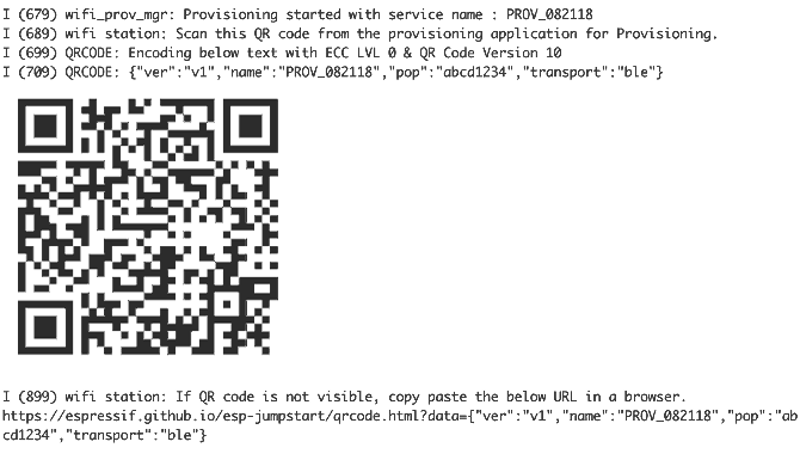
\includegraphics[width=0.9\textwidth]{D7Z/7-44}
    \caption{Log output if device not provisioned}
\end{figure}

If the device has been provisioned, you will see the following log:

\begin{codebloc}
\fontsize{9.7pt}{9.7pt}\selectfont
\begin{tabular}{d}
\vspace{2pt}
\begin{verbatim}
I (399) wifi station: Application driver initialization   
I (399) gpio: GPIO[9]| InputEn: 1| OutputEn: 0| OpenDrain: 0| Pullup: 1| Pulldown: 
0| Intr:0 
I (429) wifi station: NVS Flash initialization   
I (429) wifi station: Wi-Fi initialization   
I (549) wifi station: Wi-Fi Provisioning initialization   
I (549) wifi station: Already provisioned, starting Wi-Fi STA   
I (809) wifi station: wifi_station_initialize finished.   
\end{verbatim}
\verb|I (1939) wifi station: got ip:192.168.3.105|
\end{tabular}
\end{codebloc}

\section{Summary}
In this chapter, we first introduced two important technologies for network configuration of IoT devices, Wi-Fi and Bluetooth. Then we covered some concepts and mechanisms of Wi-Fi network configuration, including SoftAP, SmartConfig, Bluetooth, direct network configuration, RouterConfig, ZeroConfig, and phone AP network configuration. We also analysed the code for SoftAP, SmartConfig, and Bluetooth network configuration, combined with Wi-Fi programming. Finally, we tried out smart Wi-Fi configuration with the Smart Light project.

\end{document}